%%
%DIF LATEXDIFF DIFFERENCE FILE


%% This is file `sample-acmsmall-conf.tex',
%% generated with the docstrip utility.
%%
%% The original source files were:
%%
%% samples.dtx  (with options: `acmsmall-conf')
%% 
%% IMPORTANT NOTICE:
%% 
%% For the copyright see the source file.
%% 
%% Any modified versions of this file must be renamed
%% with new filenames distinct from sample-acmsmall-conf.tex.
%% 
%% For distribution of the original source see the terms
%% for copying and modification in the file samples.dtx.
%% 
%% This generated file may be distributed as long as the
%% original source files, as listed above, are part of the
%% same distribution. (The sources need not necessarily be
%% in the same archive or directory.)
%%
%%
%% Commands for TeXCount
%TC:macro \cite [option:text,text]
%TC:macro \citep [option:text,text]
%TC:macro \citet [option:text,text]
%TC:envir table 0 1
%TC:envir table* 0 1
%TC:envir tabular [ignore] word
%TC:envir displaymath 0 word
%TC:envir math 0 word
%TC:envir comment 0 0
%%
%%
%% The first command in your LaTeX source must be the \documentclass
%% command.
%%
%% For submission and review of your manuscript please change the
%% command to \documentclass[manuscript, screen, review]{acmart}.
%%
%% When submitting camera ready or to TAPS, please change the command
%% to \documentclass[sigconf]{acmart} or whichever template is required
%% for your publication.
%%
%%
\documentclass[manuscript,acmsmall,anonymous,review,screen,nonacm=true, authorversion=true,drafttrue]{acmart}

%%
%% \BibTeX command to typeset BibTeX logo in the docs
\AtBeginDocument{%
  \providecommand\BibTeX{{%
    Bib\TeX}}}

%% Rights management information.  This information is sent to you
%% when you complete the rights form.  These commands have SAMPLE
%% values in them; it is your responsibility as an author to replace
%% the commands and values with those provided to you when you
%% complete the rights form.
\setcopyright{acmcopyright}
\copyrightyear{2018}
\acmYear{2018}
\acmDOI{XXXXXXX.XXXXXXX}

%% These commands are for a PROCEEDINGS abstract or paper.
\acmConference[Conference acronym 'XX]{Make sure to enter the correct
  conference title from your rights confirmation emai}{June 03--05,
  2018}{Woodstock, NY}
%%
%%  Uncomment \acmBooktitle if the title of the proceedings is different
%%  from ``Proceedings of ...''!
%%
%%\acmBooktitle{Woodstock '18: ACM Symposium on Neural Gaze Detection,
%%  June 03--05, 2018, Woodstock, NY}
\acmPrice{15.00}
\acmISBN{978-1-4503-XXXX-X/18/06}


%%
%% Submission ID.
%% Use this when submitting an article to a sponsored event. You'll
%% receive a unique submission ID from the organizers
%% of the event, and this ID should be used as the parameter to this command.
%%\acmSubmissionID{123-A56-BU3}

%%
%% For managing citations, it is recommended to use bibliography
%% files in BibTeX format.
%%
%% You can then either use BibTeX with the ACM-Reference-Format style,
%% or BibLaTeX with the acmnumeric or acmauthoryear sytles, that include
%% support for advanced citation of software artefact from the
%% biblatex-software package, also separately available on CTAN.
%%
%% Look at the sample-*-biblatex.tex files for templates showcasing
%% the biblatex styles.
%%

%%
%% The majority of ACM publications use numbered citations and
%% references.  The command \citestyle{authoryear} switches to the
%% "author year" style.
%%
%% If you are preparing content for an event
%% sponsored by ACM SIGGRAPH, you must use the "author year" style of
%% citations and references.
%% Uncommenting
%% the next command will enable that style.
%%\citestyle{acmauthoryear}

\usepackage{booktabs}   %% For formal tables:
                        %% http://ctan.org/pkg/booktabs
\usepackage{subcaption} %% For complex figures with subfigures/subcaptions
                        %% http://ctan.org/pkg/subcaption

\usepackage{hhline}
%%%%%%%%%%%%%%%%%%%%%%%%%%%%%%%%%%%%%%%%%%%%%%%%%%%%%%%%%%%%%%%%%%%%%%%%%%%%%%%%%%%%%%%%%%%%%%%%%%%%%%%%%%%%%%%%%%%%%%%%%%%%%%%%%%%%%%%%%
%%%%%%%%%%%%%%%%%%%%%%%%%%%%%%%%%%%%%%%%%%%%%%%%%%%%% COMMANDS FOR GENERAL PAPER WRITING %%%%%%%%%%%%%%%%%%%%%%%%%%%%%%%%%%%%%%%%%%%%%%%%%%%%
%%%%%%%%%%%%%%%%%%%%%%%%%%%%%%%%%%%%%%%%%%%%%%%%%%%%%%%%%%%%%%%%%%%%%%%%%%%%%%%%%%%%%%%%%%%%%%%%%%%%%%%%%%%%%%%%%%%%%%%%%%%%%%%%%%%%%%%%%


%%%%%%%%%%%%%%%%%%%%%%%%%%%% Theorem, Definition and Proof
\newtheorem{lem}{Lemma}[section]
\newtheorem{thm}{Theorem}[section]
\newtheorem{defn}{Definition}
\newtheorem{coro}{Corollary}[thm]

\newtheorem{lemma}{Lemma}
\newtheorem{corollary}{Corollary}
\newtheorem*{theorem}{Theorem}
\renewcommand\thelemma{\unskip}
\renewcommand\thecorollary{\unskip}

% \theoremstyle{remark}
% \newtheorem*{lemma}{Lemma}

\newtheorem{example}{Example}[section]

\newcommand{\completeness}[1]{{\color{blue}\textbf{[[ #1 ]]}}}
\newcommand{\caseL}[1]{\item \textbf{case: #1}\newline}
\newcommand{\subcaseL}[1]{\item \textbf{sub-case: #1}\newline}
\newcommand{\subsubcaseL}[1]{\item \textbf{subsub-case: #1}\newline}
\newcommand{\subsubsubcaseL}[1]{\item \textbf{subsubsub-case: \boldmath{#1}}\newline}

\newcommand{\blue}[1]{{\tiny \color{blue}{ #1 }}}


\let\originalleft\left
\let\originalright\right
\renewcommand{\left}{\mathopen{}\mathclose\bgroup\originalleft}
\renewcommand{\right}{\aftergroup\egroup\originalright}
\newcommand{\ts}[1]{ \llparenthesis {#1} \rrparenthesis }

\theoremstyle{definition}

\newtheorem{case}{Case}
\newtheorem{subcase}{Case}
\numberwithin{subcase}{case}
\newtheorem{subsubcase}{Case}
\numberwithin{subsubcase}{subcase}

\newtheorem{subsubsubcase}{Case}
\numberwithin{subsubsubcase}{subsubcase}
\newcommand{\st}{~.~}
\newcommand{\sthat}{~.~}

%%%%COLORS
\definecolor{periwinkle}{rgb}{0.8, 0.8, 1.0}
\definecolor{powderblue}{rgb}{0.69, 0.88, 0.9}
\definecolor{sandstorm}{rgb}{0.93, 0.84, 0.25}
\definecolor{trueblue}{rgb}{0.0, 0.45, 0.81}

\newlength\Origarrayrulewidth
% horizontal rule equivalent to \cline but with 2pt width
\newcommand{\Cline}[1]{%
 \noalign{\global\setlength\Origarrayrulewidth{\arrayrulewidth}}%
 \noalign{\global\setlength\arrayrulewidth{2pt}}\cline{#1}%
 \noalign{\global\setlength\arrayrulewidth{\Origarrayrulewidth}}%
}

% draw a vertical rule of width 2pt on both sides of a cell
\newcommand\Thickvrule[1]{%
  \multicolumn{1}{!{\vrule width 2pt}c!{\vrule width 2pt}}{#1}%
}

% draw a vertical rule of width 2pt on the left side of a cell
\newcommand\Thickvrulel[1]{%
  \multicolumn{1}{!{\vrule width 2pt}c|}{#1}%
}

% draw a vertical rule of width 2pt on the right side of a cell
\newcommand\Thickvruler[1]{%
  \multicolumn{1}{|c!{\vrule width 2pt}}{#1}%
}

\newenvironment{subproof}[1][\proofname]{%
  \renewcommand{\qedsymbol}{$\blacksquare$}%
  \begin{proof}[#1]%
}{%
  \end{proof}%
}
%%%%%%%%%%%%%%%%%%%%%%%%%%%%%%% Fonts Definition %%%%%%%%%%%%%%%%%%%%%%%%%%%
\newcommand{\omitthis}[1]{}

% Misc.
\newcommand{\etal}{\textit{et al.}}
\newcommand{\bump}{\hspace{3.5pt}}

% Text fonts
\newcommand{\tbf}[1]{\textbf{#1}}

% Math fonts
\newcommand{\mbb}[1]{\mathbb{#1}}
\newcommand{\mbf}[1]{\mathbf{#1}}
\newcommand{\mrm}[1]{\mathrm{#1}}
\newcommand{\mtt}[1]{\mathtt{#1}}
\newcommand{\mcal}[1]{\mathcal{#1}}
\newcommand{\mfrak}[1]{\mathfrak{#1}}
\newcommand{\msf}[1]{\mathsf{#1}}
\newcommand{\mscr}[1]{\mathscr{#1}}

\newcommand{\diam}{{\color{red}\diamond}}
\newcommand{\dagg}{{\color{blue}\dagger}}
\let\oldstar\star
\renewcommand{\star}{\oldstar}

\newcommand{\im}[1]{\ensuremath{#1}}

\newcommand{\kw}[1]{\im{\mathtt{#1}}}
\newcommand{\set}[1]{\im{\{{#1}\}}}

\newcommand{\mmax}{\ensuremath{\mathsf{max}}}

%%%%%%%%%%%%%%%%%%%%%%%%%%%%%%% Blocks Definition %%%%%%%%%%%%%%%%%%%%%%%%%%%
\tikzstyle{decision} = [diamond, draw, fill=blue!20, 
    text width=4.5em, text badly centered, node distance=3cm, inner sep=0pt]
% \tikzstyle{block} = [rectangle, draw, fill=blue!20, 
%     text width=5em, text centered, rounded corners, minimum height=4em]
\tikzstyle{block} = [draw, very thick, fill=white, rectangle, 
    minimum height=2.5em, minimum width=6em, text centered]

\tikzstyle{line} = [draw, -latex']
\tikzstyle{cloud} = [draw, ellipse,fill=red!20, node distance=3cm,    minimum height=2em]

\tikzstyle{vecArrow} = [thick, decoration={markings,mark=at position
  1 with {\arrow[semithick]{open triangle 60}}},
  double distance=1.4pt, shorten >= 5.5pt,
  preaction = {decorate},
  postaction = {draw,line width=1.4pt, white,shorten >= 4.5pt}]
\tikzstyle{innerWhite} = [semithick, white,line width=1.4pt, shorten >= 4.5pt]



%%%%%%%%%%%%%%%%%%%%%%%%%%%%%%%%%%%%%%%%%%%%%%%%%%%%%%%%%%%%%%%%%%%%%%%%%%%%%%%%%%%%%%%%%%%%%%%%%%%%%%%%%%%%%%%%%%%%%%%%%%%%%%%%%%%%%%%%%%%%%%%%%%%%%%%%%%
%%%%%%%%%%%%%%%%%%%%%%%%%%%%%%%%%%%%%%%%%%%%%%%%%%%%%%%%%%%% Introduction %%%%%%%%%%%%%%%%%%%%%%%%%%%%%%%%%%%%%%%%%%%%%%%%%%%%%%%%%%%%%%%%
%%%%%%%%%%%%%%%%%%%%%%%%%%%%%%%%%%%%%%%%%%%%%%%%%%%%%%%%%%%%%%%%%%%%%%%%%%%%%%%%%%%%%%%%%%%%%%%%%%%%%%%%%%%%%%%%%%%%%%%%%%%%%%%%%%%%%%%%%%%%%%%%%%%%%%%%%%

\newcommand{\dist}{P}
\newcommand{\mech}{M}
\newcommand{\univ}{\mathcal{X}}
\newcommand{\anyl}{A}
\newcommand{\qrounds}{r}
\newcommand{\answer}{a}
\newcommand{\sample}{X}
\newcommand{\ex}[2]{{\ifx&#1& \mathbb{E} \else \underset{#1}{\mathbb{E}} \fi \left[#2\right]}}
\newcommand{\pr}[2]{{\ifx&#1& \mathbb{P} \else \underset{#1}{\mathbb{P}} \fi \left[#2\right]}}
\newcommand{\var}[2]{{\ifx&#1& \mathrm{Var} \else \underset{#1}{\mathrm{Var}} \fi \left[#2\right]}}
\newcommand{\eps}{\varepsilon}
\newcommand{\from}{:}
\newcommand{\sep}{ \ | \ }


%%%%%%%%%%%%%%%%%%%%%%%%%%%%%%%%%%%%%%%%%%%%%%%%%%%%%%%%%%%%%%%%%%%%%%%%%%%%%%%%%%%%%%%%%%%%%%%%%%%%%%%%%%%%%%%%%%%%%%%%%%%%%%%%%%%%%%%%%%%%%%%%%%%%%%%%%%
%%%%%%%%%%%%%%%%%%%%%%%%%%%%%%%%%%%%%%%%%%%%%%%%%%%%%%%%%%%% Query While Language %%%%%%%%%%%%%%%%%%%%%%%%%%%%%%%%%%%%%%%%%%%%%%%%%%%%%%%%%%%%%%%%
%%%%%%%%%%%%%%%%%%%%%%%%%%%%%%%%%%%%%%%%%%%%%%%%%%%%%%%%%%%%%%%%%%%%%%%%%%%%%%%%%%%%%%%%%%%%%%%%%%%%%%%%%%%%%%%%%%%%%%%%%%%%%%%%%%%%%%%%%%%%%%%%%%%%%%%%%%
% Language
\newcommand{\command}{c}
%Label
\newcommand{\lin}{\kw{in}}
\newcommand{\lex}{\kw{ex}}
% expression
\newcommand{\expr}{e}
\newcommand{\aexpr}{a}
\newcommand{\bexpr}{b}
\newcommand{\sexpr}{\ssa{\expr} }
\newcommand{\qexpr}{\psi}
\newcommand{\qval}{\alpha}
\newcommand{\query}{{\tt query}}
\newcommand{\eif}{\;\kw{if}\;}
\newcommand{\ethen}{\kw{\;then\;}}
\newcommand{\eelse}{\kw{\;else\;}} 
\newcommand{\eapp}{\;}
\newcommand{\eprojl}{\kw{fst}}
\newcommand{\eprojr}{\kw{snd}}
\newcommand{\eifvar}{\kw{ifvar}}
\newcommand{\ewhile}{\;\kw{while}\;}
\newcommand{\bop}{\;*\;}
\newcommand{\uop}{\;\circ\;}
\newcommand{\eskip}{\kw{skip}}
\newcommand{\edo}{\;\kw{do}\;}
% More unary expression operators:
\newcommand{\esign}{~\kw{sign}~}
\newcommand{\elog}{~\kw{log}~}


\newcommand{\emax}{~\kw{max}~}
\newcommand{\emin}{~\kw{min}~}


%%%%%%%%%% Extended
\newcommand{\efun}{~\kw{fun}~}
\newcommand{\ecall}{~\kw{call}~}


% Domains
\newcommand{\qdom}{\mathcal{QD}}
\newcommand{\memdom}{\mathcal{M}}
\newcommand{\dbdom}{\mathcal{DB}}
\newcommand{\cdom}{\mathcal{C}}
\newcommand{\ldom}{\mathcal{L}}

\newcommand{\emap}{~\kw{map}~}
\newcommand{\efilter}{~\kw{filter}~}

%configuration
\newcommand{\config}[1]{\langle #1 \rangle}
\newcommand{\ematch}{\kw{match}}
\newcommand{\clabel}[1]{\left[ #1 \right]}

\newcommand{\etrue}{\kw{true}}
\newcommand{\efalse}{\kw{false}}
\newcommand{\econst}{c}
\newcommand{\eop}{\delta}
\newcommand{\efix}{\mathop{\kw{fix}}}
\newcommand{\elet}{\mathop{\kw{let}}}
\newcommand{\ein}{\mathop{ \kw{in}} }
\newcommand{\eas}{\mathop{ \kw{as}} }
\newcommand{\enil}{\kw{nil}}
\newcommand{\econs}{\mathop{\kw{cons}}}
\newcommand{\term}{t}
\newcommand{\return}{\kw{return}}
\newcommand{\bernoulli}{\kw{bernoulli}}
\newcommand{\uniform}{\kw{uniform}}
\newcommand{\app}[2]{\mathrel{ {#1} \, {#2} }}


% Operational Semantics
\newcommand{\env}{\rho}
\newcommand{\rname}[1]{\textsf{\small{#1}}}
\newcommand{\aarrow}{\Downarrow_a}
\newcommand{\barrow}{\Downarrow_b}
\newcommand{\earrow}{\Downarrow_e}
\newcommand{\qarrow}{\Downarrow_q}
\newcommand{\cmd}{c}
\newcommand{\node}{N}
\newcommand{\assign}[2]{ \mathrel{ #1  \leftarrow #2 } }


%%%%%%%%%%%%%%%%%%%%%%%%%%%%%%%%%%%%%%%%%%%%%%%%%%%%%%%%%%%%%%%%%%%%%%%% Trace and Events %%%%%%%%%%%%%%%%%%%%%%%%%%%%%%%%%%%%%%%%
%%%%%%%%%%%%%%%%%%%%%%%%%%%%%%%%%%%%%%%%%%%%%%%%%%%%%%%%%%%%%%%%%%%%%% Trace 
%%%%%%%% annotated query
\newcommand{\aq}{\kw{aq}}
\newcommand{\qtrace}{\kw{qt}}
%annotated variables
\newcommand{\av}{\kw{av}}
\newcommand{\vtrace}{\kw{\tau}}
\newcommand{\ostrace}{{\kw{\tau}}}
\newcommand{\posttrace}{{\kw{\tau}}}



%%%%%%%%%%%%%%%%%traces
\newcommand{\tdom}{\mathcal{T}^{+\infty}}
\newcommand{\trace}{\kw{\tau}}
\newcommand{\ftdom}{\mathcal{T}^{+}}
\newcommand{\inftdom}{\mathcal{T}^{\infty}}

% \newcommand{\vcounter}{\kw{\zeta}}
\newcommand{\vcounter}{\kw{cnt}}

\newcommand{\postevent}{{\kw{\epsilon}}}


\newcommand{\event}{\kw{\epsilon}}
\newcommand{\eventset}{\mathcal{E}}
\newcommand{\eventin}{\in_{\kw{e}}}
\newcommand{\eventeq}{=_{\kw{e}}}
\newcommand{\eventneq}{\neq_{\kw{e}}}
\newcommand{\eventgeq}{\geq_{\kw{e}}}
\newcommand{\eventlt}{<_{\kw{e}}}
\newcommand{\eventleq}{\leq_{\kw{e}}}
\newcommand{\eventdep}{\mathsf{DEP_{\kw{e}}}}
\newcommand{\asn}{\kw{{asn}}}
\newcommand{\test}{\kw{{test}}}
\newcommand{\ctl}{\kw{{ctl}}}

\newcommand{\sig}{\kw{sig}}
\newcommand{\sigeq}{=_{\sig}}
\newcommand{\signeq}{\neq_{\sig}}
\newcommand{\notsigin}{\notin_{\sig}}
\newcommand{\sigin}{\in_{\sig}}
\newcommand{\sigdiff}{\kw{Diff}_{\sig}}
\newcommand{\action}{\kw{act}}
\newcommand{\diff}{\kw{Diff}}
\newcommand{\seq}{\kw{seq}}
\newcommand{\sdiff}{\kw{Diff}_{\seq}}

\newcommand{\tracecat}{{\scriptscriptstyle ++}}
\newcommand{\traceadd}{{\small ::}}

\newcommand{\ism}{\kw{ism}}
\newcommand{\ismdiff}{\kw{Diff}_{\sig}}
\newcommand{\ismeq}{=_{\ism}}
\newcommand{\ismneq}{\neq_{\ism}}
\newcommand{\notismin}{\notin_{\ism}}
\newcommand{\ismin}{\in_{\ism}}

%operations on the trace and Annotated Query
\newcommand{\projl}[1]{\kw{\pi_{l}(#1)}}
\newcommand{\projr}[1]{\kw{\pi_{r}(#1)}}

% operations on annotated query, i.e., aq
\newcommand{\aqin}{\in_{\kw{aq}}}
\newcommand{\aqeq}{=_{\kw{aq}}}
\newcommand{\aqneq}{\neq_{\kw{aq}}}
\newcommand{\aqgeq}{\geq_{\kw{aq}}}

% operations on annotated variables, i.e., av
\newcommand{\avin}{\in_{\kw{av}}}
\newcommand{\aveq}{=_{\kw{av}}}
\newcommand{\avneq}{\neq_{\kw{av}}}
\newcommand{\avgeq}{\geq_{\kw{av}}}
\newcommand{\avlt}{<_{\kw{av}}}

% adaptivity
\newcommand{\adap}{\kw{adap}}
\newcommand{\ddep}[1]{\kw{depth}_{#1}}
\newcommand{\nat}{\mathbb{N}}
\newcommand{\natb}{\nat_{\bot}}
\newcommand{\natbi}{\natb^\infty}
\newcommand{\nnatA}{Z}
\newcommand{\nnatB}{m}
\newcommand{\nnatbA}{s}
\newcommand{\nnatbB}{t}
\newcommand{\nnatbiA}{q}
\newcommand{\nnatbiB}{r}


%%%%%%%%%%%%%%%%%%%%%%%%%%%%%%%%%%%%%%%%%%%%%%%%%%%%%%%%%%%%%%%%%%%%%%%%%%%%%%%%%%%%%%%%%%%%%%%%%%%%%%%%%%%%%%%%%%%%%%%%%%%%%%%%%%%%%%%%%%%%%%%%%%%%%%%%%%
%%%%%%%%%%%%%%%%%%%%%%%%%%%%%%%%%%%%%%%%%%%%%%%%%%%%%%%%%%%% Semantic Definition %%%%%%%%%%%%%%%%%%%%%%%%%%%%%%%%%%%%%%%%%%%%%%%%%%%%%%%%%%%%%%%%
%%%%%%%%%%%%%%%%%%%%%%%%%%%%%%%%%%%%%%%%%%%%%%%%%%%%%%%%%%%%%%%%%%%%%%%%%%%%%%%%%%%%%%%%%%%%%%%%%%%%%%%%%%%%%%%%%%%%%%%%%%%%%%%%%%%%%%%%%%%%%%%%%%%%%%%%%%

%%%%%%%%%%%%%%%%%%%%%%%%%%%%%%%%% Semantics Based Dependency, Graph and Adaptivity 
\newcommand{\paths}{\mathcal{PATH}}
\newcommand{\walks}{\mathcal{WK}}
\newcommand{\progwalks}{\mathcal{WK}^{\kw{est}}}

\newcommand{\len}{\kw{len}}
\newcommand{\lvar}{\mathbb{LV}}
\newcommand{\avar}{\mathbb{AV}}
\newcommand{\qvar}{\mathbb{QV}}
\newcommand{\qdep}{\mathsf{DEP_{q}}}
\newcommand{\vardep}{\mathsf{DEP_{var}}}
\newcommand{\avdep}{\mathsf{DEP_{\av}}}
\newcommand{\finitewalk}{\kw{fw}}
\newcommand{\pfinitewalk}{\kw{fwp}}
\newcommand{\dep}{\mathsf{DEP}}

\newcommand{\llabel}{\iota}
\newcommand{\entry}{\kw{entry}}
\newcommand{\tlabel}{\mathbb{TL}}

\newcommand{\traceG}{\kw{{G_{trace}}}}
\newcommand{\traceV}{\kw{{V_{trace}}}}
\newcommand{\traceE}{\kw{{E_{trace}}}}
\newcommand{\traceF}{\kw{{Q_{trace}}}}
\newcommand{\traceW}{\kw{{W_{trace}}}}

%%%%%%%%%%%%%%%%%%%%%%%%%%%%%%%%%%%%%%%%%%%%%%%%%%%%%%%%%%%%%%%%%%%%%%%%%%%%%%%%%%%%%%%%%%%%%%%%%%%%%%%%%%%%%%%%%%%%%%%%%%%%%%%%%%%%%%%%%%%%%%%%%%%%%%%%%%
%%%%%%%%%%%%%%%%%%%%%%%%%%%%%%%%%%%%%%%%%%%%%%%%%%%%%%%%%%%% Static Program Analysis %%%%%%%%%%%%%%%%%%%%%%%%%%%%%%%%%%%%%%%%%%%%%%%%%%%%%%%%%%%%%%%%
%%%%%%%%%%%%%%%%%%%%%%%%%%%%%%%%%%%%%%%%%%%%%%%%%%%%%%%%%%%%%%%%%%%%%%%%%%%%%%%%%%%%%%%%%%%%%%%%%%%%%%%%%%%%%%%%%%%%%%%%%%%%%%%%%%%%%%%%%%%%%%%%%%%%%%%%%%

%Static Adaptivity Definition:
\newcommand{\flowsto}{\kw{flowsTo}}
\newcommand{\live}{\kw{RD}}

%Analysis Algorithms and Graphs
\newcommand{\weight}{\mathsf{W}}
\newcommand{\green}[1]{{ \color{green} #1 } }

\newcommand{\func}[2]{\mathsf{AD}(#1) \to (#2)}
\newcommand{\varCol}{\bf{VetxCol}}
\newcommand{\graphGen}{\bf{FlowGen}}
\newcommand{\progG}{\kw{{G_{est}}}}
\newcommand{\progV}{\kw{{V_{est}}}}
\newcommand{\progE}{\kw{{E_{est}}}}
\newcommand{\progF}{\kw{{Q_{est}}}}
\newcommand{\progW}{\kw{{W_{est}}}}
\newcommand{\progA}{{\kw{A_{est}}}}

\newcommand{\midG}{\kw{{G_{mid}}}}
\newcommand{\midV}{\kw{{V_{mid}}}}
\newcommand{\midE}{\kw{{E_{mid}}}}
\newcommand{\midF}{\kw{{Q_{mid}}}}



\newcommand{\sccgraph}{\kw{G^{SCC}}}
\newcommand{\sccG}{\kw{{G_{scc}}}}
\newcommand{\sccV}{\kw{{V_{scc}}}}
\newcommand{\sccE}{\kw{{E_{scc}}}}
\newcommand{\sccF}{\kw{{Q_{scc}}}}
\newcommand{\sccW}{\kw{{W_{scc}}}}


\newcommand{\visit}{\kw{visit}}

\newcommand{\flag}{\kw{F}}
\newcommand{\Mtrix}{\kw{M}}
\newcommand{\rMtrix}{\kw{RM}}
\newcommand{\lMtrix}{\kw{LM}}
\newcommand{\vertxs}{\kw{V}}
\newcommand{\qvertxs}{\kw{QV}}
\newcommand{\qflag}{\kw{Q}}
\newcommand{\edges}{\kw{E}}
\newcommand{\weights}{\kw{W}}
\newcommand{\qlen}{\len^{\tt q}}
\newcommand{\pwalks}{\mathcal{WK}_{\kw{p}}}

\newcommand{\rb}{\mathsf{RechBound}}
\newcommand{\pathsearch}{\mathsf{AdaptSearch}}

%program abstraction
\newcommand{\abst}[1]{\kw{abs}{#1}}
\newcommand{\absexpr}{\abst{\kw{expr}}}
% \newcommand{\absevent}{\stackrel{\scriptscriptstyle{\alpha}}{\event{}}}
\newcommand{\absevent}{\hat{\event{}}}
\newcommand{\absfinal}{\abst{\kw{final}}}
\newcommand{\absinit}{\abst{\kw{init}}}
\newcommand{\absflow}{\abst{\kw{trace}}}
\newcommand{\absG}{\abst{\kw{G}}}
\newcommand{\absV}{\abst{\kw{V}}}
\newcommand{\absE}{\abst{\kw{E}}}
\newcommand{\absF}{\abst{\kw{F}}}
\newcommand{\absW}{\abst{\kw{W}}}
\newcommand{\locbound}{\kw{locb}}
\newcommand{\absdom}{\mathcal{ADOM}}

\newcommand{\inpvar}{\vardom_{\kw{in}}}
\newcommand{\grdvar}{\vardom_{\kw{guard}}}
\newcommand{\vardom}{\mathcal{V}}
\newcommand{\inpvardom}{\mathcal{V}_{\kw{\lin}}}
\newcommand{\scexprdom}{\mathcal{A}_{\kw{sc}}}
\newcommand{\inpexprdom}{\mathcal{A}_{\lin}}
\newcommand{\scvardom}{\mathcal{SC}}
\newcommand{\valuedom}{\mathcal{VAL}}
\newcommand{\scexpr}{{\kw{A_{sc}}}}


\newcommand{\absclr}{{\kw{TB}}}
\newcommand{\varinvar}{{\kw{VB}}}
\newcommand{\init}{\kw{init}}
\newcommand{\constdom}{\mathcal{SC}}
\newcommand{\dcdom}{\mathcal{DC}}
\newcommand{\reset}{\kw{re}}
\newcommand{\resetchain}{\kw{rechain}}
\newcommand{\inc}{\kw{inc}}
\newcommand{\dec}{\kw{dec}}
\newcommand{\booldom}{\mathcal{B}}
\newcommand{\incrs}{\kw{increase}}




%%%%%%%%%%%%%%%%%%%%%%%%%%%%%%%%%%%%%%%%%%%%%%%%%%%%%%%%%%%%%%%%%%%%%%%%%%%%%%%%%%%%%%%%%%%%%%%%%%%%%%%%%%%%%%%%%%%%%%%%%%%%%%%%%%%%%%%%%%%%%%%%%%%%%%%%%%
%%%%%%%%%%%%%%%%%%%%%%%%%%%%%%%%%%%%%%%%%%%%%%%%%%%%%%%%%%%%%%%%%%%%%%% author comments in draft mode %%%%%%%%%%%%%%%%%%%%%%%%%%%%%%%%%%%%%%%%%%%%%%%%%%%%%%%%%%%%%%%%%%%%%%
%%%%%%%%%%%%%%%%%%%%%%%%%%%%%%%%%%%%%%%%%%%%%%%%%%%%%%%%%%%%%%%%%%%%%%%%%%%%%%%%%%%%%%%%%%%%%%%%%%%%%%%%%%%%%%%%%%%%%%%%%%%%%%%%%%%%%%%%%%%%%%%%%%%%%%%%%%

\newif\ifdraft
%\draftfalse
\drafttrue

\newcommand{\todo}[1]{{\color{red}\textbf{[[ #1 ]]}}}
% \newcommand{\todo}[1]{#1}
\newcommand{\todomath}[1]{{\scriptstyle \color{red}\mathbf{[[ #1 ]]}}}


\ifdraft
% Jiawen
\newcommand{\jl}[1]{\textcolor[rgb]{.00,0.00,1.00}{[JL: #1]}}
% \newcommand{\jl}[1]{#1}
\newcommand{\jlside}[1]{\marginpar{\tiny \sf \textcolor[rgb]{.00,0.80,0.00}{[jl: #1]}}}
% Deepak
\newcommand{\dg}[1]{\textcolor[rgb]{.00,0.80,0.00}{[DG: #1]}}
\newcommand{\dgside}[1]{\marginpar{\tiny \sf \textcolor[rgb]{.00,0.80,0.00}{[DG: #1]}}}
% Marco
\newcommand{\mg}[1]{\textcolor[rgb]{.80,0.00,0.00}{[MG: #1]}}
\newcommand{\mgside}[1]{\marginpar{\tiny \sf \textcolor[rgb]{.80,0.00,0.00}{[MG: #1]}}}
% Weihao
\newcommand{\wq}[1]{\textcolor[rgb]{.00,0.80,0.00}{[WQ: #1]}}
\newcommand{\wqside}[1]{\marginpar{\tiny \sf \textcolor[rgb]{.00,0.80,0.00}{[WQ: #1]}}}
\else
\newcommand{\mg}[1]{}
\newcommand{\mgside}[1]{}
\newcommand{\wq}[1]{}
\newcommand{\wqside}[1]{}
\newcommand{\rname}[1]{$\textbf{#1}$}
\fi

\newcommand{\highlight}[1]{\textcolor[rgb]{.0,0.0,1.0}{ #1}}
% \newcommand{\highlight}[1]{{ #1}}

\newcommand{\THESYSTEM}{\textsf{AdaptFun}}

%%
%% end of the preamble, start of the body of the document source.
%DIF PREAMBLE EXTENSION ADDED BY LATEXDIFF
%DIF UNDERLINE PREAMBLE %DIF PREAMBLE
\RequirePackage[normalem]{ulem} %DIF PREAMBLE
\RequirePackage{color}\definecolor{RED}{rgb}{1,0,0}\definecolor{BLUE}{rgb}{0,0,1} %DIF PREAMBLE
\providecommand{\DIFadd}[1]{{\protect\color{blue}\uwave{#1}}} %DIF PREAMBLE
\providecommand{\DIFdel}[1]{{\protect\color{red}\sout{#1}}}                      %DIF PREAMBLE
%DIF SAFE PREAMBLE %DIF PREAMBLE
\providecommand{\DIFaddbegin}{} %DIF PREAMBLE
\providecommand{\DIFaddend}{} %DIF PREAMBLE
\providecommand{\DIFdelbegin}{} %DIF PREAMBLE
\providecommand{\DIFdelend}{} %DIF PREAMBLE
\providecommand{\DIFmodbegin}{} %DIF PREAMBLE
\providecommand{\DIFmodend}{} %DIF PREAMBLE
%DIF FLOATSAFE PREAMBLE %DIF PREAMBLE
\providecommand{\DIFaddFL}[1]{\DIFadd{#1}} %DIF PREAMBLE
\providecommand{\DIFdelFL}[1]{\DIFdel{#1}} %DIF PREAMBLE
\providecommand{\DIFaddbeginFL}{} %DIF PREAMBLE
\providecommand{\DIFaddendFL}{} %DIF PREAMBLE
\providecommand{\DIFdelbeginFL}{} %DIF PREAMBLE
\providecommand{\DIFdelendFL}{} %DIF PREAMBLE
%DIF END PREAMBLE EXTENSION ADDED BY LATEXDIFF

\begin{document}

%%
%% The "title" command has an optional parameter,
%% allowing the author to define a "short title" to be used in page headers.
\title[short]{Program Analysis for Adaptive Data Analysis}  

%%
%% The "author" command and its associated commands are used to define
%% the authors and their affiliations.
%% Of note is the shared affiliation of the first two authors, and the
%% "authornote" and "authornotemark" commands
%% used to denote shared contribution to the research.
% \author{Ben Trovato}
% \authornote{Both authors contributed equally to this research.}
% \email{trovato@corporation.com}
% \orcid{1234-5678-9012}
% \author{G.K.M. Tobin}
% \authornotemark[1]
% \email{webmaster@marysville-ohio.com}
% \affiliation{%
%   \institution{Institute for Clarity in Documentation}
%   \streetaddress{P.O. Box 1212}
%   \city{Dublin}
%   \state{Ohio}
%   \country{USA}
%   \postcode{43017-6221}
% }

% \author{Lars Th{\o}rv{\"a}ld}
% \affiliation{%
%   \institution{The Th{\o}rv{\"a}ld Group}
%   \streetaddress{1 Th{\o}rv{\"a}ld Circle}
%   \city{Hekla}
%   \country{Iceland}}
% \email{larst@affiliation.org}

% \author{Valerie B\'eranger}
% \affiliation{%
%   \institution{Inria Paris-Rocquencourt}
%   \city{Rocquencourt}
%   \country{France}
% }

% \author{Aparna Patel}
% \affiliation{%
%  \institution{Rajiv Gandhi University}
%  \streetaddress{Rono-Hills}
%  \city{Doimukh}
%  \state{Arunachal Pradesh}
%  \country{India}}

% \author{Huifen Chan}
% \affiliation{%
%   \institution{Tsinghua University}
%   \streetaddress{30 Shuangqing Rd}
%   \city{Haidian Qu}
%   \state{Beijing Shi}
%   \country{China}}

% \author{Charles Palmer}
% \affiliation{%
%   \institution{Palmer Research Laboratories}
%   \streetaddress{8600 Datapoint Drive}
%   \city{San Antonio}
%   \state{Texas}
%   \country{USA}
%   \postcode{78229}}
% \email{cpalmer@prl.com}

% \author{John Smith}
% \affiliation{%
%   \institution{The Th{\o}rv{\"a}ld Group}
%   \streetaddress{1 Th{\o}rv{\"a}ld Circle}
%   \city{Hekla}
%   \country{Iceland}}
% \email{jsmith@affiliation.org}

% \author{Julius P. Kumquat}
% \affiliation{%
%   \institution{The Kumquat Consortium}
%   \city{New York}
%   \country{USA}}
% \email{jpkumquat@consortium.net}

%%
%% By default, the full list of authors will be used in the page
%% headers. Often, this list is too long, and will overlap
%% other information printed in the page headers. This command allows
%% the author to define a more concise list
%% of authors' names for this purpose.
% \renewcommand{\shortauthors}{Trovato et al.}

%%
%% The abstract is a short summary of the work to be presented in the
%% article.
\begin{abstract}
  Data analyses are usually designed to identify some property of the population from which the data are drawn, generalizing beyond the specific data sample. For this reason, data analyses are often designed in a way that guarantees that they produce a low generalization error.
  That is, they are designed so that the result of a data analysis run on a sample data does not differ too much from the result one would achieve by running the analysis over the entire population. 

  An adaptive data analysis can be seen as a process composed by multiple queries interrogating some data, where the choice of which query to run next may rely on the results of previous queries. 
  The generalization error of each individual query/analysis can be controlled by using an array of well-established statistical techniques.
  However, when queries are arbitrarily composed, the different errors can propagate through the chain of different queries and bring to a high generalization error. 
  To address this issue, data analysts are designing several techniques that not only guarantee bounds on the generalization errors of single queries, but that also guarantee bounds on the generalization error of the composed analyses. 
  The choice of which of these techniques to use, often depends on the chain of queries that an adaptive data analysis can generate.

  In this work, we consider adaptive data analyses implemented as while-like programs and we design a program analysis which can help with identifying which technique to use to control their generalization errors. 
  More specifically, we formalize the intuitive notion of \emph{adaptivity} as a quantitative property of programs. 
  We do this because the adaptivity level of a data analysis is a key measure to choose the right technique. 
  Based on this definition, we design a program analysis for soundly approximating this quantity.
  The program analysis generates a representation of the data analysis as a weighted dependency graph, where the weight is an upper bound on the number of times each variable can be reached, and uses a path search strategy to guarantee an upper bound on the adaptivity. 
  We implement our program analysis  and show that it can help to analyze the adaptivity of several concrete data analyses with different adaptivity structures.
  \end{abstract}

%%
%% The code below is generated by the tool at http://dl.acm.org/ccs.cfm.
%% Please copy and paste the code instead of the example below.
%%
% \begin{CCSXML}
% <ccs2012>
%  <concept>
%   <concept_id>00000000.0000000.0000000</concept_id>
%   <concept_desc>Do Not Use This Code, Generate the Correct Terms for Your Paper</concept_desc>
%   <concept_significance>500</concept_significance>
%  </concept>
%  <concept>
%   <concept_id>00000000.00000000.00000000</concept_id>
%   <concept_desc>Do Not Use This Code, Generate the Correct Terms for Your Paper</concept_desc>
%   <concept_significance>300</concept_significance>
%  </concept>
%  <concept>
%   <concept_id>00000000.00000000.00000000</concept_id>
%   <concept_desc>Do Not Use This Code, Generate the Correct Terms for Your Paper</concept_desc>
%   <concept_significance>100</concept_significance>
%  </concept>
%  <concept>
%   <concept_id>00000000.00000000.00000000</concept_id>
%   <concept_desc>Do Not Use This Code, Generate the Correct Terms for Your Paper</concept_desc>
%   <concept_significance>100</concept_significance>
%  </concept>
% </ccs2012>
% \end{CCSXML}

% \ccsdesc[500]{Do Not Use This Code~Generate the Correct Terms for Your Paper}
% \ccsdesc[300]{Do Not Use This Code~Generate the Correct Terms for Your Paper}
% \ccsdesc{Do Not Use This Code~Generate the Correct Terms for Your Paper}
% \ccsdesc[100]{Do Not Use This Code~Generate the Correct Terms for Your Paper}

%%
%% Keywords. The author(s) should pick words that accurately describe
%% the work being presented. Separate the keywords with commas.
\keywords{Adaptive data analysis, program analysis, dependency graph}
%% A "teaser" image appears between the author and affiliation
%% information and the body of the document, and typically spans the
%% page.
% \begin{teaserfigure}
%   \includegraphics[width=\textwidth]{sampleteaser}
%   \caption{Seattle Mariners at Spring Training, 2010.}
%   \Description{Enjoying the baseball game from the third-base
%   seats. Ichiro Suzuki preparing to bat.}
%   \label{fig:teaser}
% \end{teaserfigure}

\received{20 February 2007}
\received[revised]{12 March 2009}
\received[accepted]{5 June 2009}

%%
%% This command processes the author and affiliation and title
%% information and builds the first part of the formatted document.
\maketitle

%%%%%%%%%%%%%%%%%%%%%%%%%%%%%%%%%%%%%%%%%%% Introduction and Overview %%%%%%%%%%%%%%%%%%%%%%%%%%%%%%%%%%%%%%%%%%% 
\section{Introduction}
\label{sec:intro}
% The topic, motivation, the importance of adaptivity 
Consider a dataset $X$ consisting of $n$ independent samples from some unknown population $\dist$.  How can we ensure that the conclusions drawn from $X$ \emph{generalize} to the population $\dist$?  Despite decades of research in statistics and machine learning on methods for ensuring generalization, there is an increased recognition that many scientific findings generalize poorly (e.g. 
\cite{Ioannidis05,GelmanL13}). While there are many reasons a conclusion might fail to generalize, one that is receiving increasing attention is \emph{adaptivity}, which occurs when the choice of method for analyzing the dataset depends on previous interactions with the same dataset~\cite{GelmanL13}.
%
 Adaptivity can arise from many common practices, such as exploratory data analysis, using the same data set for feature selection and regression, and the re-use of datasets across research projects.  Unfortunately, adaptivity invalidates traditional methods for ensuring generalization and statistical validity, which assume that the method is selected independently of the data. The misinterpretation of adaptively selected results has even been blamed for a ``statistical crisis'' in empirical science~\cite{GelmanL13}.
%  ~\cite{GelmanL13}.

\begin{figure}
    \centering
    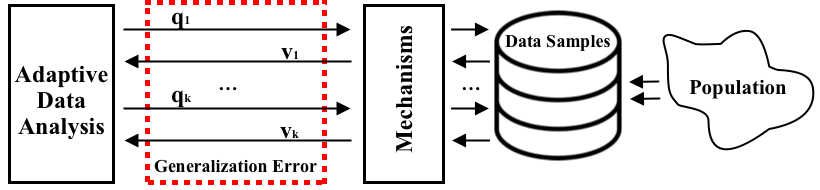
\includegraphics[width=0.7\columnwidth]{overview.png}
    \caption{Overview of our Adaptive Data Analysis model. We have a population that we are interested in studying, and a dataset containing individual samples from this population. The adaptive data analysis we are interested in running has access to the dataset through queries of some pre-determined family (e.g., statistical or linear queries) mediated by a mechanism. This mechanism uses randomization to reduce the generalization error of the queries issued to the data.}
    \label{fig:adaptivity-model-overview}
\vspace{-0.5cm}
\end{figure}

A line of work initiated by \citet{DworkFHPRR15}, \citet{HardtU14} posed the question: Can we design \emph{general-purpose} methods that ensure generalization in the presence of adaptivity, together with guarantees on their accuracy?  The idea that has emerged in these works is to use randomization to help ensure generalization. Specifically, these works have proposed to mediate the access of an adaptive data analysis to the data by means of queries from some pre-determined family (we will consider here a specific family of queries often called "statistical" or "linear" queries) that are sent to a  \emph{mechanism} which uses some randomized process to guarantee that the result of the query does not depend too much on the specific
sampled dataset. This guarantees that the result of the queries generalizes well. This approach is described in Fig.~\ref{fig:adaptivity-model-overview}.  
This line of work has identified many new algorithmic techniques for ensuring generalization in adaptive data analysis, leading to algorithms with greater statistical power than all previous approaches. Common methods proposed by these works include, the addition of noise to the result of a query, data splitting, using sampling methods, etc. Moreover, these works have also identified problematic strategies for adaptive analysis, showing limitations on the statistical power one can hope to achieve. Subsequent works have then further extended the methods and techniques in this approach and further extended the theoretical underpinning of this approach, e.g.~\cite{dwork2015reusable,dwork2015generalization,BassilyNSSSU16,UllmanSNSS18,FeldmanS17,jung2019new,SteinkeZ20,RogersRSSTW20,DaganK22,Blanc23}.


A key development in this line of work is that the best method for ensuring generalization in an adaptive data analysis depends to a large extent on the number of \emph{rounds of adaptivity}, the depth of the chain of queries. As an informal example, the program $x \leftarrow q_1(D);y \leftarrow q_2(D,x);z \leftarrow q_3(D,y)$ has three rounds of adaptivity, since $q_2$  depends on $D$ not only directly because it is one of its input but also via the result of $q_1$, which is also run on $D$, and similarly,  $q_3$ depends on $D$ directly but also via the result of $q_2$, which in turn depends on the result of $q_1$. The works we discussed above showed that, not only does the analysis of the generalization error depend on the number of rounds, but knowing the number of rounds actually allows one to choose methods that lead to the smallest possible generalization error\DIFdelbegin \DIFdel{- we will discuss this further in Section~\ref{sec:overview}. 
}%DIFDELCMD < 

%DIFDELCMD < %%%
\DIFdel{For example}\DIFdelend \DIFaddbegin \DIFadd{. 
For instance}\DIFaddend , these works showed that when an adaptive data analysis uses a large number of rounds of adaptivity\DIFaddbegin \DIFadd{, }\DIFaddend then a low generalization error can be achieved by \DIFdelbegin \DIFdel{a }\DIFdelend \DIFaddbegin \DIFadd{the Gaussian }\DIFaddend mechanism  
adding to the result of each query Gaussian noise scaled to the number of rounds. When instead  an adaptive data analysis uses a small number of rounds of adaptivity then a low generalization error can be achieved by using more specialized methods, such as \DIFaddbegin \DIFadd{the }\DIFaddend data splitting mechanism or the reusable holdout technique from~\citet{DworkFHPRR15}.
%DIF <  \detailed{To better understand this idea, we show in Fig.~\raef{fig:generalization_errors} two experiments showcasing these situations. More precisely, in Fig.~\ref{fig:generalization_errors}(a) we show the results of a specific analysis\footnote{We will use formally a program implementing this analysis (Fig.~\ref{fig:overview-example}) as a running example in the rest of the paper.} with two rounds of adaptivity. This analysis can be seen as a classifier which first runs 500 non-adaptive queries on the first 500 attributes of the data, looking for correlations between the attributes and a label, and then runs one last query which depends on all these correlations. Without any mechanism the generalization error is pretty large, and the lower generalization error is achieved when the data-splitting method is used. 
%DIF >  \detailed{To better understand this idea, we show in Fig.~\ref{fig:generalization_errors} two experiments showcasing these situations. More precisely, in Fig.~\ref{fig:generalization_errors}(a) we show the results of a specific analysis\footnote{We will use formally a program implementing this analysis (Fig.~\ref{fig:overview-example}) as a running example in the rest of the paper.} with two rounds of adaptivity. This analysis can be seen as a classifier which first runs 500 non-adaptive queries on the first 500 attributes of the data, looking for correlations between the attributes and a label, and then runs one last query which depends on all these correlations. Without any mechanism the generalization error is pretty large, and the lower generalization error is achieved when the data-splitting method is used. 
% In Fig.~\ref{fig:generalization_errors}(b), we show the results of a specific analysis\footnote{We will present this analysis formally in Section~\ref{sec:examples}.} with four hundreds rounds of adaptivity. This analysis can be seen as a classifier which at each step runs an adaptive query based on the result of the previous ones. Again, without any mechanism the generalization error is pretty large, and the lower generalization error is achieved when the Gaussian noise is used.}
%DIF >  \highlight{TO DO: A more detailed explanation of the three adpativity mechanisms}.
%DIF >  To better understand this idea, we show in Fig.~\ref{fig:generalization_errors} three experiments showcasing these situations. More precisely, in Fig.~\ref{fig:generalization_errors}(a) we show the results of a specific analysis\footnote{We will use formally a program implementing this analysis (Fig.~\ref{fig:overview-example}) as a running example in the rest of the paper.} with two rounds of adaptivity. This analysis can be seen as a classifier which first runs 400 non-adaptive queries on the first 400 attributes of the data, looking for correlations between the attributes and a label, and then runs one last query which depends on all these correlations. Without any mechanism the generalization error of the last query is pretty large, and the lower generalization error is achieved when the data-splitting method is used. Fig.~\ref{fig:generalization_errors}(c) shows how this situation also changes with the number of queries. Specifically, it shows the root mean square error of the last \emph{adaptive} query when the number of queries varies. This also highlights the fact that different mechanisms, for the same analysis, produce results with different generalization errors.
%DIF >  In Fig.~\ref{fig:generalization_errors}(a) and Fig.~\ref{fig:generalization_errors}(c) we  use the same analysis but different data sizes. This is mostly to account for 
%DIF >  the fact that we run many more queries in Fig.~\ref{fig:generalization_errors}(c). Using a larger data set in Fig.~\ref{fig:generalization_errors}(c) also changes the magnitude of the error. 
\DIFaddbegin 

\DIFaddend To better understand this idea, we show in Fig.~\ref{fig:generalization_errors} three experiments showcasing these situations\DIFdelbegin \DIFdel{. More precisely, in }\DIFdelend \DIFaddbegin \DIFadd{: 
%DIF >  \highlight{Fig.~\ref{fig:generalization_errors}(a) shows the generalization errors of one adaptive data analysis program with the adaptivity $2$ when no mechinism(marked as overfitted), Gaussian mechanism(guassian noise) and Data splitting mechanism(data splitting) are applied;
%DIF >   Fig.~\ref{fig:generalization_errors}(b) shows the generalization errors of one adaptive data analysis under similar three conditions as Fig.~\ref{fig:generalization_errors}(a), the difference is the adapativity is $400$ instead of $2$;
%DIF >    Fig.~\ref{fig:generalization_errors}(c) shows how the generalization errors also change along with the number of queries when various mechanisms are applied.} 
%DIF >  More precisely,  
In }\DIFaddend Fig.~\ref{fig:generalization_errors}(a) we show the results of a specific analysis\footnote{We will use formally a program implementing this analysis (Fig.~\ref{fig:overview-example}) as a running example in the rest of the paper.} 
with two rounds of adaptivity.
 \DIFdelbegin \DIFdel{This analysis can be seen as a classifier which first runs 400 non-adaptive queries on the first 400 attributes of the data, looking for correlations between the attributes and a label, and then runs one last query which depends on all these correlations. Without any mechanism the generalization error of the last query is pretty large, and the lower generalization error is achieved when the data-splitting method is used. Fig.~\ref{fig:generalization_errors}(c) shows how this situation also changes with the number of queries. Specifically, it shows the root mean square error of the last }\emph{\DIFdel{adaptive}} %DIFAUXCMD
\DIFdel{query when the number of queries varies. This also highlights the fact that different mechanisms, for the same analysis, produce results with different generalization errors.
}\DIFdelend \DIFaddbegin \highlight{This analysis can be seen as a classifier for a population where individuals samples consist of 400 attributes and 1 label. Using a dataset representing a sample from this population, this analysis first runs 400 non-adaptive queries on the first 400 attributes of the dataset,
  computing correlations between each attribute and the label. Then, it runs the last query depending on all these correlations. The adaptivity of this analysis is $2$ because only the last query relies on the results of the previous queries' results. 
  Without any mechanism the generalization error of the last query may be pretty large, and we can achieve lower generalization error by using the data-splitting method. 
  In Fig.~\ref{fig:generalization_errors}(c), we use the same data analysis program as in Fig.~\ref{fig:generalization_errors}(a). It runs over a dataset with larger data size and shows only the root mean square error of the last \emph{adaptive} query when the 
total query number varies along the x-axis. This figure is meant to show how the total number of queries also affect the generalization error.
Fig.~\ref{fig:generalization_errors}(c) also highlights the fact that different mechanisms, for the same analysis, produce results with different generalization errors, and
using a larger data set changes the magnitude of the error. } 
\DIFaddend In Fig.~\ref{fig:generalization_errors}(\DIFdelbegin \DIFdel{a) and Fig.~\ref{fig:generalization_errors}(c) we  use the same analysis but different data sizes. This is mostly to account for 
the fact that we run many more queries in Fig.~\ref{fig:generalization_errors}(c). Using a larger data set in Fig.~\ref{fig:generalization_errors}(c) also changes the magnitude of the error. 
In Fig.~\ref{fig:generalization_errors}(}\DIFdelend b), we show the results of a specific analysis\footnote{We will present this analysis formally in Section~\ref{sec:examples}.} with four \DIFdelbegin \DIFdel{hundreds }\DIFdelend \DIFaddbegin \DIFadd{hundred }\DIFaddend rounds of adaptivity.
At each step, this analysis runs an adaptive query based on the results of the previous ones. Without any mechanism, the generalization error of most of the queries is pretty large, and this error can be lowered by using Gaussian noise. 
\DIFaddbegin \highlight{Overall, in Fig.~\ref{fig:generalization_errors} we use  three different mechanisms: the Gaussian mechanism which adds to the result of each query Gaussian noise; the Data Splitting mechanism
that splits the data into a few parts on which runs independently the different queries; the Thresholdout mechanism that uses the reusable holdout technique from~\citet{DworkFHPRR15}.  }
\DIFaddend {\small
\begin{figure}
\centering
\begin{subfigure}{.322\textwidth}
\begin{centering}
\DIFdelbeginFL %DIFDELCMD < 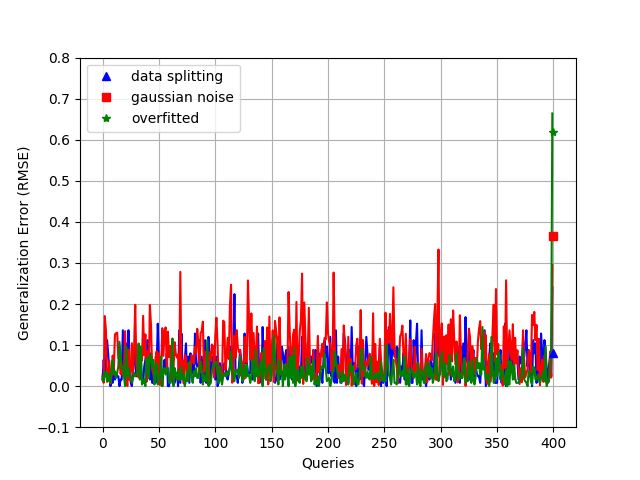
\includegraphics[width=0.7\textwidth]{tworound.png}
%DIFDELCMD < %%%
\DIFdelendFL \DIFaddbeginFL 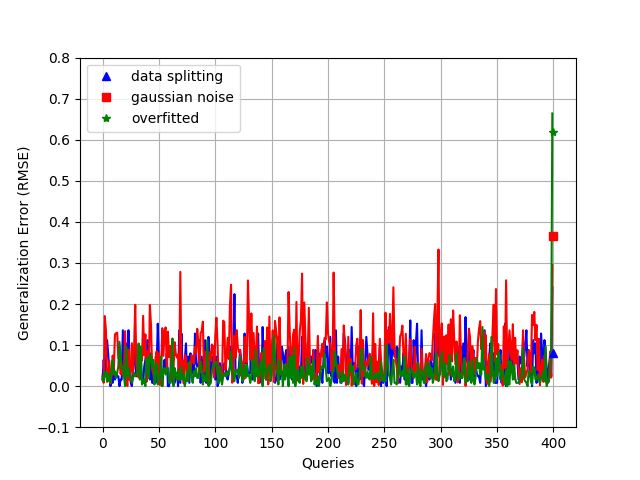
\includegraphics[width=1.0\textwidth]{tworound.png}
\DIFaddendFL \caption{}
\end{centering}
\end{subfigure}
\quad
\begin{subfigure}{.322\textwidth}
\begin{centering}
\DIFdelbeginFL %DIFDELCMD < 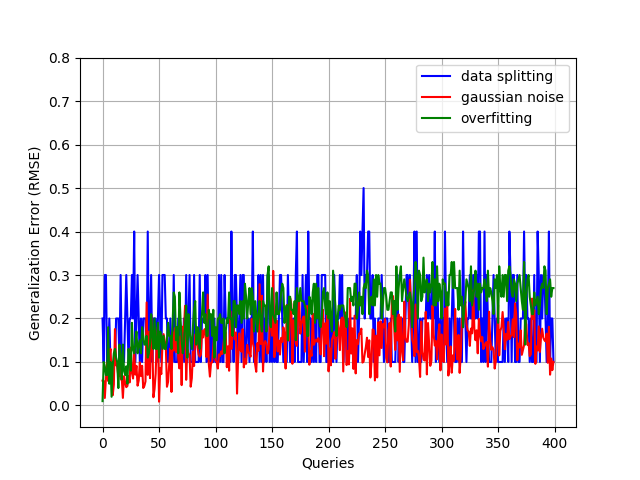
\includegraphics[width=0.7\textwidth]{multipleround.png}
%DIFDELCMD < %%%
\DIFdelendFL \DIFaddbeginFL 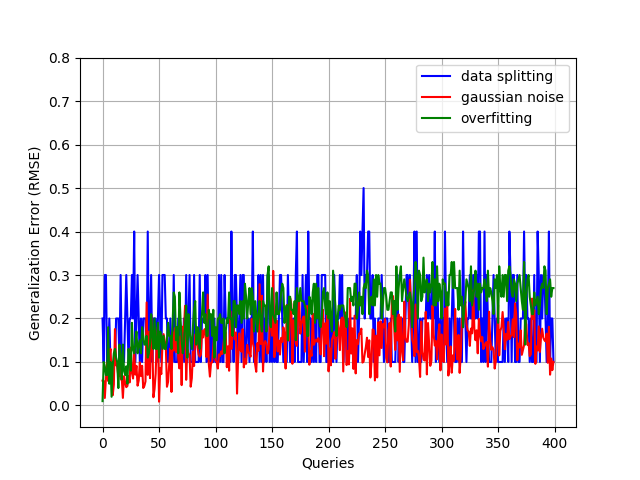
\includegraphics[width=1.0\textwidth]{multipleround.png}
\DIFaddendFL \caption{}
\end{centering}
\end{subfigure}
\begin{subfigure}{.322\textwidth}
\begin{centering}
\DIFdelbeginFL %DIFDELCMD < 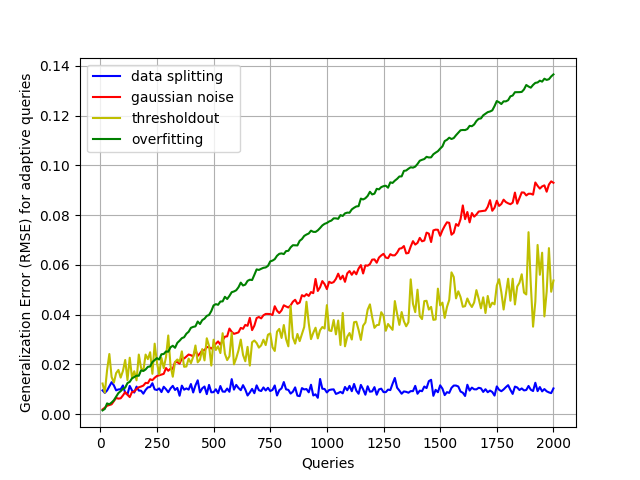
\includegraphics[width=0.7\textwidth]{twoRounds-rmse-fourmechs.png}
%DIFDELCMD < %%%
\DIFdelendFL \DIFaddbeginFL 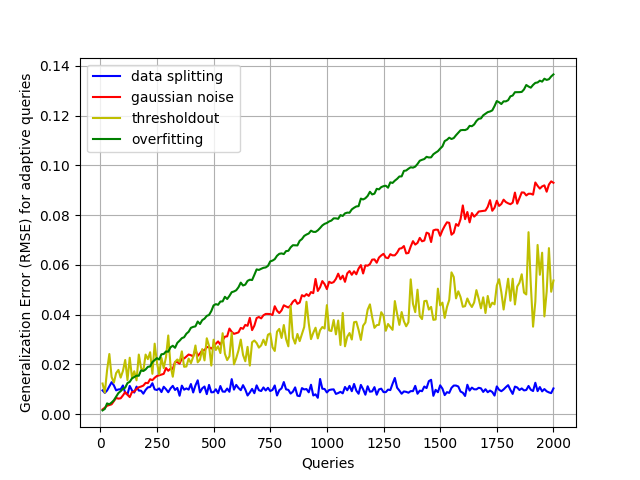
\includegraphics[width=1.0\textwidth]{twoRounds-rmse-fourmechs.png}
\DIFaddendFL \caption{}
\end{centering}
\end{subfigure}
\vspace{-0.2cm}
 \caption{
 The generalization errors of two adaptive data analysis examples, under different choices of mechanisms.
 (a)  2 rounds adaptivity. 
 (b)  400 rounds adaptivity.
 (c) 2 rounds adaptivity with varied query numbers.
}
\label{fig:generalization_errors}
\vspace{-0.2cm}
\end{figure}
}
%gap

This scenario motivates us to explore the design of program analysis techniques that can be used to estimate the number of \emph{rounds of adaptivity} that a program implementing a data analysis can perform. These techniques could be used to help a data analyst in the choice of the mechanism to use,
and they
could ultimately be integrated into a tool for adaptive data analysis such as the \emph{Guess and Check} framework by~\citet{RogersRSSTW20}. 

The first problem we face is \emph{how to formally define} a model for adaptive data analysis which is general enough to support the methods we discussed above and which would permit to formulate the notion of adaptivity these methods use. We take the approach of designing a programming framework for submitting queries to some \emph{mechanism} giving access to the data mediated by one of the techniques we mentioned before, e.g., adding Gaussian noise, randomly selecting a subset of the data, using the reusable holdout technique, etc. In this approach, a program models an \emph{analyst} asking a sequence of queries to the mechanism. The mechanism runs the queries on the data applying one of the methods above and returns the result to the program. The program can then use this result to decide which query to run next. Overall, we are interested in controlling the generalization error of the query results returned by the mechanism, by means of the adaptivity. 

The second problem we face is \emph{how to define the adaptivity of a given program}.
Intuitively, a query $Q$ may depend on another query $P$, if there are two values that $P$ can return which affect in different ways the execution of $Q$. 
For example, as shown in \cite{dwork2015reusable}, and as we did in our example in Fig.~\ref{fig:generalization_errors}(a), one can design a machine learning algorithm for constructing a classifier which first computes each feature's correlation with the label via a sequence of queries, and then constructs the classifier based on the correlation values. If one feature's correlation changes, the classifier depending on features is also affected.  
This notion of dependency builds on the execution trace as a \emph{causal history}. In particular, we are interested in the history or provenance of a query up until this is executed, \DIFaddbegin \DIFadd{and }\DIFaddend we are not then concerned about how the result is used --- except for tracking whether the result of the query may further cause some other queries. This is because we focus on the generalization error of queries and not their post-processing. % 
To formalize this intuition as a quantitative program property,
we use a trace semantics recording the execution history of programs on some given input --- and we create a dependency graph, where the dependency between different variables (queries are also assigned to variables) is explicit and tracks which variable is associated with a query request. We then enrich this graph with weights describing the number of times each variable is evaluated in a program evaluation starting with an initial state. The adaptivity is then defined as the length of the walk visiting \DIFaddbegin \DIFadd{the }\DIFaddend most query-related variables on this graph\footnote{Formally, graphs will be well-defined only for terminating programs, this will guarantee that the walk is finite}. In other words, we define adaptivity as a \emph{quantitative form of program dependency}.

% \jl{ 
% To define adaptivity in our programming framework, we consider a weighted dependency graph over variables assigned in the program, where each edge is built by a semantics dependency relation between these variables. The dependency relation relies on the trace semantics of our programming framework which records the execution history of programs implementing adaptive data analysis. 
% %The novelty comes from the definition of relation of dependency between nodes, which consists of the edge in the graph. For now, we can think of each node is associated with a variable, storing the value assigned to its variable 
% }
% \jl{The general idea beneath this dependency relation is that modifying the value of some variable in an execution trace will later affect the following execution trace.
% By tracking if a variable is assigned by a query or not, we are able to distinguish whether one query may depend on the other.}

The third problem we face is \emph{how to estimate the adaptivity of a given program}. 
The adaptive data analysis model we consider and our definition of adaptivity suggest that for this task we can use a  program analysis that is based on some form of dependency analysis. This analysis needs to take into consideration:
1) the fact that, in general, a query $Q$ is not a monolithic block but rather it may depend, through the use of variables and values, on other parts of the program. Hence, it needs to consider some form of data flow analysis. 
2) the fact that, in general, the decision on whether to run a query or not may depend on some other value. Hence, 
 it needs to consider some form of control flow analysis.
 3) the fact that, in general, we are not only interested in whether there is a dependency or not, but in the length of the chain of dependencies. Hence, it needs to consider some quantitative information about the program dependencies. 

To address these considerations and be able to estimate a sound upper bound on the adaptivity of a program, 
we develop a static program analysis algorithm, named {\THESYSTEM}, which combines data flow and control flow analysis with reachability bound analysis~\cite{GulwaniZ10}. This combination gives tighter bounds on the adaptivity of a program than the ones one would achieve by directly using the data and control flow analyses or the ones that one would achieve by directly using reachability bound analysis techniques alone. We evaluate {\THESYSTEM} on a number of examples showing that it is able to efficiently estimate precise upper bounds on the adaptivity of different programs. 
All the proofs and extended definitions can be found in the supplementary material.

To summarize, our work aims at the design of a static analysis for programs implementing adaptive analysis that can estimate their rounds of adaptivity. Specifically, our contributions are:
\begin{enumerate}
    \item A programming framework for adaptive data analyses where programs represent analysts that can query generalization-preserving mechanisms mediating the access to some data. 
    \item 
    A formal definition of the notion of adaptivity under the analyst-mechanism model,
    built on a variable-based dependency graph constructed using sets of program execution traces.
    \item 
    A static program analysis algorithm {\THESYSTEM} combining data flow, control flow and  reachability bound analysis in order to provide tight bounds on the adaptivity of a program.
    \item A soundness proof of the program analysis showing that the adaptivity estimated by {\THESYSTEM} bounds the true adaptivity of the program. 
    \item A prototype implementation of {\THESYSTEM} and an experimental evaluation showing its accuracy and efficiency of the adaptivity estimation on several examples.  
    We also provide an evaluation showing how the generalization error of several real-world data analyses can be effectively reduced by using the information provided by {\THESYSTEM}.
\end{enumerate}
\DIFaddbegin 

\DIFaddend \section{Overview}
\label{sec:overview}
\subsection{Some results in Adaptive Data Analysis}
%\wq{I think we can move this subsection into appendix. Maybe just leave theorm 1.2 and 1.3}
%\jl{I don't agree}
In Adaptive Data Analysis, an \emph{analyst} is interested in studying some distribution $\dist$ over some domain $\univ$.  Following previous works~\cite{DworkFHPRR15,HardtU14,BassilyNSSSU16}, we focus on the setting where the analyst is interested in answers to \emph{statistical queries} (also known as \emph{linear queries}) over the distribution.  A statistical query is usually defined by some function $\qquery \from \univ \to [-1,1]$ (often other codomains such as $[0,1]$ or $[-R,+R]$, for some $R$, are considered).  The analyst wants to learn the \emph{population mean}, which is defined as 
$\qquery(\dist) = \ex{\sample \sim \dist}{\qquery(\sample)}$. 
%
We assume that the distribution $\dist$ can only be accessed via a set of \emph{samples} $\sample_1,\dots,\sample_n$ drawn independently and identically distributed (i.i.d.) from $\dist$.  These samples are held by a mechanism $\mech(\sample_1,\dots,\sample_n)$ who receives the query $\qquery$ and computes an answer 
$\answer \approx \qquery(\dist)$.
%
The na\"ive way to approximate the population mean is to use the \emph{empirical mean}, which (abusing notation) is defined as 
$\qquery(\sample_1,\dots,\sample_n) = \frac{1}{n} \sum_{i=1}^{n} \qquery(X_i)$.
However, the mechanism $M$ can adopt some methods for improving the generalization error $| a- \qquery(\dist)|$.

In this work we consider analysts that ask a sequence of $k$ queries $\qquery_1,\dots,\qquery_k$.  If the queries are all chosen in advance, independently of the answers $a_1,\dots,a_k$ of each other, then we say they are \emph{non-adaptive}.  If the choice of each query $\qquery_j$ depends on the prefix $\qquery_1,\answer_1,\dots,\qquery_{j-1},\answer_{j-1}$ then they are \emph{fully adaptive}.  An important intermediate notion is \emph{$\qrounds$-round adaptive}, where the sequence can be partitioned into $\qrounds$ batches of non-adaptive queries.  Note that non-adaptive queries are $1$-round and fully adaptive queries are $k$-round adaptive.

We now review what is known about the problem of answering $r$-round adaptive queries.  
\begin{thm}[\cite{BassilyNSSSU16}] 
\label{thm:nonadapt-adapt}
\begin{enumerate}

\item For any distribution $\dist$, and any $k$ \emph{non-adaptive} statistical queries, with high \DIFdelbegin \DIFdel{probablity}\DIFdelend \DIFaddbegin \DIFadd{probability}\DIFaddend ,
% $$
$
\max_{j=1,\dots,k} | \answer_j - \qquery_j(\dist) | = O\left( \sqrt{\frac{\log k}{n}}  \right)
% $$
$.
%
\item For any distribution $\dist$, and  any $k$  \emph{$\qrounds$-round adaptive} statistical queries, with $\qrounds \geq 2$, with high \DIFdelbegin \DIFdel{probablity}\DIFdelend \DIFaddbegin \DIFadd{probability}\DIFaddend , the empirical mean (rounded to an appropriate number of bits of precision)\footnote{With infinite precision even two queries may give unbounded error, when the first query's result encodes the whole data.} satisfies:\\
% $$
$
\max_{j=1,\dots,k} | \answer_j - \qquery_j(\dist) | = O\left( \sqrt{  \frac{k}{n}}  \right)
% $$
$
\end{enumerate}
\end{thm}
In fact, these bounds are tight (up to constant factors) which means that even allowing one extra round of adaptivity leads to an exponential increase in the generalization error, from $\log k$ to $k$.

\citet{DworkFHPRR15} and \citet{BassilyNSSSU16} showed that by using carefully calibrated Gaussian noise in order to limit the dependency of a single query on the specific data instance, one 
can actually achieve much stronger generalization error as a function of the number of queries, specifically.
\begin{thm}[\cite{DworkFHPRR15, BassilyNSSSU16}] \label{thm:gaussiannoise} For any distribution $\dist$, any $k$, any $\qrounds \geq 2$ and any \emph{$\qrounds$-round adaptive} statistical queries, if we answer queries with carefully calibrated Gaussian noise, with high \DIFdelbegin \DIFdel{probablity}\DIFdelend \DIFaddbegin \DIFadd{probability}\DIFaddend ,  we have:
\begin{center}
  $
\max_{j=1,\dots,k} | \answer_j - \qquery_j(\dist) | = O\left( \frac{\sqrt[4]{k}}{\sqrt{n}}  \right)
$  
\end{center}
\end{thm}
% Notice that in order to Theorem~\ref{thm:gaussiannoise} has different quantification in that the optimal choice of mechanism depends on the number of queries.  Thus, we need to know the number of queries \emph{a priori} to choose the best mechanism.
More interestingly, \citet{DworkFHPRR15}
also gave a refined bounds that can be achieved with different mechanisms depending on the number of rounds of adaptivity.   \begin{thm}[\cite{DworkFHPRR15}] \label{thm:gaussiannoise2} For any $r$ and $k$, there exists a mechanism such that for any distribution $\dist$, and any $\qrounds \geq 2$ any \emph{$\qrounds$-round adaptive} statistical queries, with high \DIFdelbegin \DIFdel{probablity}\DIFdelend \DIFaddbegin \DIFadd{probability}\DIFaddend , it satisfies
\begin{center}
  $
\max_{j=1,\dots,k} | \answer_j - \qquery_j(\dist) | = O\left( \frac{r \sqrt{\log k}}{\sqrt{n}}  \right)
$  
\end{center}
\end{thm}
Notice that Theorem~\ref{thm:gaussiannoise2} has different quantification in that the optimal choice of mechanism depends on the number of queries {and number of rounds of adaptivity}.  This suggests that if one knows a good \emph{a priori upper bound on the number of rounds of adaptivity}, one can choose the appropriate mechanism and get a much better guarantee in terms of the generalization error.
As an example, as we can see in Fig.~\ref{fig:generalization_errors}, if we know that an algorithm is 2-rounds adaptive, we can choose data splitting as {the} mechanism, while if we know that an algorithm has many rounds of adaptivity we can choose Gaussian noise. It is worth to \DIFdelbegin \DIFdel{stress }\DIFdelend \DIFaddbegin \DIFadd{stressing }\DIFaddend that by knowing the number of rounds of adaptivity one can also compute a concrete upper bound on the generalization error of a data analysis. This information allows one to have a quantitative, a priori, estimation of the effectiveness of a data analysis. 
This motivates us to design a static program analysis aimed at giving good \emph{a priori} upper bounds on the number of rounds of adaptivity of a program. 

{\small
\begin{figure}
\centering
\begin{subfigure}{.2\textwidth}
\begin{centering}
$
    \begin{array}{l}
    \kw{towRounds(k)} \triangleq \\
           \clabel{ \assign{a}{0}}^{0} ;
            \clabel{\assign{j}{k} }^{1} ; \\
            \ewhile ~ \clabel{j > 0}^{2} ~ \edo ~ \\
            \Big(
             \clabel{\assign{x}{\query(\chi[j] \cdot \chi[k])} }^{3}  ; \\
             \clabel{\assign{j}{j-1}}^{4} ;\\
            \clabel{\assign{a}{x + a}}^{5}       \Big);\\
            \clabel{\assign{l}{\query(\chi[k]*a)} }^{6}\\
        \end{array}
$
\caption{}
\end{centering}
\end{subfigure}
\begin{subfigure}{.4\textwidth}
%}
\qquad
\begin{centering}
\begin{tikzpicture}[scale=\textwidth/16cm,samples=250]
\draw[] (0, 10) circle (0pt) node
{{ $a^0: {}^{\lambda \trace_0. 1}_{0}$}};
\draw[] (0, 7) circle (0pt) node
{\textbf{$x^3: {}^{\lambda \trace_0. \env(\trace_0) k}_{1}$}};
\draw[] (0, 4) circle (0pt) node {{ $a^5: {}^{\lambda \trace_0. \env(\trace_0) k}_{0}$}};
\draw[] (0, 1) circle (0pt) node
{{ $l^6: {}^{\lambda \trace_0. 1}_{1}$}};
% Counter Variables
\draw[] (8, 9) circle (0pt) node {\textbf{$j^1: {}^{\lambda \trace_0. 1}_{0}$}};
\draw[] (8, 6) circle (0pt) node {{ $j^4: {}^{\lambda \trace_0. \env(\trace_0) k}_{0}$}};
%
% Value Dependency Edges:
\draw[ ultra thick, -latex, densely dotted,] (0, 1.5)  -- (0, 3.5) ;
\draw[ ultra thick, -latex, densely dotted,] (0, 4.5)  -- (0, 6.5) ;
\draw[ thick, -latex] (0, 4.5)  to  [out=-230,in=230]  (0, 9.5) ;
\draw[ thick, -Straight Barb] (1.5, 3.8) arc (120:-200:1);
\draw[ thick, -Straight Barb] (9, 6.5) arc (150:-150:1);
\draw[ thick, -latex] (8, 6.5)  -- (8, 8.5) ;
\draw[ thick, -latex] (0, 1.5)  to  [out=-230,in=230]  (0, 9.5) ;
% Control Dependency
\draw[ thick,-latex] (2, 7)  -- (6, 9) ;
\draw[ thick,-latex] (2, 4.5)  -- (6, 9) ;
\draw[ thick,-latex] (2, 7)  -- (6, 6) ;
\draw[ thick,-latex] (2, 4.5)  -- (6, 6) ;
\end{tikzpicture}
\caption{}
\end{centering}
\end{subfigure}
   \begin{subfigure}{.36\textwidth}
   \begin{centering}
   \begin{tikzpicture}[scale=\textwidth/18cm,samples=200]
\draw[] (0, 10) circle (0pt) node
{{ $a^0: {}^1_{0}$}};
\draw[] (0, 7) circle (0pt) node
{\textbf{$x^3: {}^{k}_{1}$}};
\draw[] (0, 4) circle (0pt) node
{{ $a^5: {}^{k}_{0}$}};
\draw[] (0, 1) circle (0pt) node
{{ $l^6: {}^{1}_{1}$}};
% Counter Variables
\draw[] (5, 9) circle (0pt) node {\textbf{$j^1: {}^{1}_{0}$}};
\draw[] (5, 6) circle (0pt) node {{ $j^4: {}^{k}_{0}$}};
%
% Value Dependency Edges:
\draw[ ultra thick, -latex, densely dotted,] (0, 1.5)  -- (0, 3.5) ;
\draw[ ultra thick, -latex, densely dotted,] (0, 4.5)  -- 
% node [left] {\highlight{$\trace_0 \to \env(\trace_0) k $}}
(0, 6.5) ;
\draw[ thick, -latex] (0, 4.5)  to  [out=-230,in=230]  
% node [left] {\highlight{$\trace_0 \to \env(\trace_0) k $}}
(0, 9.5) ;
\draw[ thick, -Straight Barb] (1.5, 3.5) arc (120:-200:1);
\draw[ thick, -Straight Barb] (6.5, 6.5) arc (150:-150:1);
    % The Weight for this edge
    % \draw[](9, 6) node [] {\highlight{$\trace_0 \to \env(\trace_0) k  $}};
\draw[ thick, -latex] (5, 6.5)  -- (5, 8.5) ;
% Control Dependency
\draw[ thick,-latex] (1.5, 7)  -- (4, 9) ;
\draw[ thick,-latex] (1.5, 4)  -- (4, 9) ;
\draw[ thick,-latex] (1.5, 7)  -- (4, 6) ;
\draw[ thick,-latex] (1.5, 4)  -- (4, 6) ;
\draw[ thick, -latex] (0, 1.5)  to  [out=-230,in=230]  (0, 9.5) ;
\end{tikzpicture}
\caption{}
   \end{centering}
   \end{subfigure}
\vspace{-0.4cm}
 \caption{(a) The program $\kw{towRounds(k)}$, an example 
%  of a program 
with two rounds of adaptivity (b) The corresponding execution-based dependency graph (c) The program-based dependency graph from $\THESYSTEM$.
}
\label{fig:overview-example}
% \vspace{-0.8cm}
\end{figure}
}


\subsection{ {\THESYSTEM} formally through an example.}
We illustrate the key technical components of our framework through a simple adaptive data analysis with two rounds of adaptivity.
% They are 1. the query while language for expressing a data analysis formally, 2. the definition of \emph{adaptivity} (\emph{adaptivity} is the short for \emph{rounds of adaptivity} used in the rest of the paper) based on the language semantics, and 3. the static analysis algorithm providing a sound upper bound on a data analysis' adaptivity.
% }
% \detailed{
% In "two rounds strategy" analysis, the analyst asks in total $k+1$ queries to the mechanism in two phases, the symbol $k$ is an input from the data analyst of this strategy and has no limit on the kind, which can be a constant, or a symbol or even an expression such as $(k+3)*2$.
% } 
%
In this analysis, an analyst asks $k+1$ queries to a mechanism in two phases.
In the first phase, the analyst asks $k$ queries and stores the answers that are provided by the mechanism. In the second phase, the analyst constructs a new query based on the results of the previous $k$ queries and sends this query to the mechanism. 
The mechanism is abstract here and our goal is to use static analysis to provide an upper bound on adaptivity to help choose the mechanism.
This data analysis assumes that the data domain $\univ$ 
contains at least $k$ numeric attributes 
(every query in the first phase focuses on one), which we index just by natural numbers.
The implementation of this data analysis in the language of {\THESYSTEM} is presented in Fig.~\ref{fig:overview-example}(a).

The {\THESYSTEM} language extends a standard while language\footnote{Programs components are labeled, so that we can uniquely identify every component.} with a query request constructor denoted $\query$.
 Queries have the form $\query(\qexpr)$, where $\qexpr$ is a special expression (see syntax in Section~\ref{sec:loop_language}) 
representing a function $\from \univ \to U$ on rows of an hidden database that is only accessible through the mechanisms. The domain $\univ$ of this function is the (arbitrary) domain of rows of the database. The codomain $U$ of this function is the query output space which, depending on the specific program, could be $[-1,1]$, $[0,1]$ or $[-R,+R]$, for some $R$. We use this formalization because we are interested in linear queries which, as we discussed in the previous section, compute the empirical mean of functions on rows.
 As an example, $x \leftarrow \query(\chi[j] \cdot \chi[k])$ computes an approximation, according to the used mechanism, of the empirical mean of the product of the $j^{th}$ attribute and $k^{th}$ attribute, identified by $\chi[j] \cdot \chi[k]$. Notice that we don't materialize the mechanism but we assume that it is implicitly run when we execute the query. 
 In Fig.~\ref{fig:overview-example}(a), the queries inside the while loop correspond to the first phase of the data analysis and compute the sum of the empirical mean of
the product of the $j$th attribute with the $k$th attribute. 
The query outside the loop corresponds to the second phase and computes an approximation of the empirical mean of the last attribute weighted by the sum of the empirical mean of the first $k$ attributes.


This example is intuitively 2-rounds adaptive since we have two clearly distinguished phases, and the queries that we ask in the first phase do not depend on each other (the query $\chi[j] \cdot \chi[k]$ at line $3$ only relies on the counter $j$ and input $k$), while the last query 
(at line 6) depends on the results of all the previous queries. 
However, capturing this concept formally is surprisingly challenging. The difficulty comes from the quantitative nature of this concept and how this quantitative nature interacts with data and control dependency. We describe how we capture it next. 
% \mg{this is weaker than it was in the previous submission.}

%%%%%%%%%%%%%%%%%%%%%%%%%%%%%%%%%%%Some details that might be useful when make passes %%%%%%%%%%%%%%%%%
% \jl{ The $\bullet$ stands for no query, for instance, the second event in the trace $(j, 1, \env(\trace)k , \bullet) $ tells us the assignment at line $1$ does not request a query.} \jl{The third event is a testing event corresponding to the guard of the while loop at line $2$. The evaluation of the query request in the second phase is tracked in }
% % \jl{ 
% The $\bullet$ is a default value for non-query event, 
% for instance, the second event in the trace $(j, 1, K , \bullet) $ tells us the assignment at line $1$ does not request a query.
% The third event is a testing event corresponding to the guard of the while loop at line $2$. The evaluation of the query request in the second phase is tracked in 
% % }
\subsubsection{Adaptivity definition}
\label{sec:adaptivity-informal}
%%%%%%%%%%%%%%%%%%%%%%%%%%%%%%%%%%% Details Below that might be useful when make passes %%%%%%%%%%%%%%%%%
% \detailed{To formally define the adaptivity, we build a directed graph representing the possible dependencies between queries of a program and we call this graph: execution-based dependency graph. The vertices represent the assigned program variables and the edges satisfy the dependency relations between vertices.   Fig.~\ref{fig:overview-example}(b) is the execution dependency graph we build based on the "two rounds strategy program" in Fig.~\ref{fig:overview-example}(a). In brief, the graph is built by collecting the assigned variables with labels of the target program as vertices, which are $a^0$, $j^1$,...$a^5$,$l^6$. We check if there is an edge between two vertices by our dependency relation over two labeled variables (defined in Section~\ref{sec:dep_adaptivity} ). This dependency relation relies on the execution of the program recorded by a trace generated by our trace semantics, which is the reason we call this graph "execution-based". 
% Intuitively from Fig.~\ref{fig:overview-example}(a), the query in the second phase (at line 6) depends on the query results in the first phase stored in $a$ at line 5, and the variable $a$ also relies on the queries at line 3. Correspondingly, we have two edges $(l^6, a^5)$ and $(a^5, x^3)$ in our execution-based dependency graph in Fig.~\ref{fig:overview-example}(b). Besides, we also have special edge which is a circle, to track any variable being updated with its previous value recursively. For instance, the counter $j$ and the variable $a$ are updated based on previous values $k$ times in the first phase and we see two circle edges on $a^5$ and $j^4$.}

The central property we are after in this work is the \emph{adaptivity of a program}. We define formally this notion in three steps (details in Section~\ref{sec:adaptivity}). First, we define a notion of dependency, or better \emph{may-dependency}, between variables. To do this we take inspiration from previous works on dependency analysis and information flow control and we say that a variable \emph{may depend} on another one if changing the execution of the latter can affect the execution of the former. 
We can see in Fig.~\ref{fig:overview-example}(a) that the value of the variable $l$, which corresponds to the result of the execution of the query in the second phase (in the command with label 6), is affected by the value of the variable $x$, which corresponds to the result of the execution of the query at line 3 in the first phase, via the variable $a$.
To formally define this notion of dependency, as in information flow control, we use the execution history of programs recorded by a trace semantics (see Definition~\ref{def:var_dep}).
% \mg{Please, double check that I refer to the right definition. }  

Second, we build an annotated weighted directed graph representing the possible dependencies between labeled variables. We call this graph \DIFaddbegin \DIFadd{the }\DIFaddend \emph{semantics-based dependency graph} to stress that this graph summarizes the dependencies we could see if we knew the overall behavior of the program. 
The vertices of the graph are the assigned program variables with the label of their assignments, edges are pairs of labeled variables which satisfy the dependency relations, weights are functions associated with vertices and describe the number of times the assignment corresponding to the vertex is executed when the program is run in a given starting state\footnote{In our trace semantics the state is recorded in the trace, so an initial state is actually represented by an initial trace. We will use this terminology in later sections.}, and the annotations, which we call \emph{query annotations}, are bits associated with vertices and describe if the corresponding assignment comes from a query (1) or not (0).
The \emph{semantics-based dependency graph} of the $\kw{twoRounds(k)}$ program
we gave in Fig.~\ref{fig:overview-example}(a) is described in Fig.~\ref{fig:overview-example}(b) (we use dashed arrows for two edges that will be highlighted in the next step, for the moment these can be considered similar to the other edges---i.e. solid arrows).
We have all the variables that are assigned in the program with their labels, and edges representing dependency relations between them. 
For example, we have two edges $(l^6, a^5)$ and $(a^5, x^3)$ describing the dependency between the variables assigned by queries. The vertices $l^6$ and $x^3$ are the only ones with query annotation $1$ (the subscript), since they are the only two variables that are in assignments involving  queries. Notice that the graph contains cycles---in this example it contains two self-loops. These cycles capture the fact that the variables $a^5$ and $j^4$ are updated at every iteration of the loop using their previous values. Cycles are essential to capture mutual dependencies like the ones that are generated in loops. Adaptivity is a quantitative notion, so capturing this form of dependencies is not enough. 
This is why we also use weights. 
\DIFdelbegin \DIFdel{The weight of a vertex is a function that given an initial state returns a natural number representing 
the number of times the assignment corresponding to a vertex is visited during the program execution starting in this initial state.  
For example, the vertex $l^{6}$ has weight }%DIFDELCMD < {%%%
\DIFdel{$\lambda \trace.1$}%DIFDELCMD < } %%%
\DIFdel{since for every initial state }%DIFDELCMD < {%%%
\DIFdel{$\trace$}%DIFDELCMD < } %%%
\DIFdel{the corresponding assignment will be executed one time, the vertex $a^5$ on the other hand has weight }%DIFDELCMD < {%%%
\DIFdel{$\lambda \trace. \env(\trace) k$ since the corresponding assignment will be executed a number of times that correspond to the value of $k$ in the initial state $\trace$, and $\env$ is the operator reading value of $k$ from $\trace$.
}%DIFDELCMD < }
%DIFDELCMD < %%%
\DIFdelend \DIFaddbegin \highlight{The weight of a vertex is a function that given an initial state returns a natural number representing 
the number of times this vertex is visited during the program execution. This number may depend on the values of the input variables, provided in the initial trace. 
For instance, in the running example in Fig.~\ref{fig:overview-example}(b), the number of times the vertex $a^5$ will be visited depends on the actual value of 
the input variable $k$. To capture this, we define a function
$\kw{lastVal}(\tau, x)$ that returns the latest value of the variable $x$ in any initial trace $\trace$.
It is natural that some vertices are visited only a constant number of times. For instance, the vertex $l^{6}$ is executed only once.
 To express this, we use the function $\kw{lastVal}$ but with a constant instead of an input variables. For example, we use $\kw{lastVal}(\tau, 1)$ as the weight for  the vertex $l^{6}$.
 In Fig.~\ref{fig:overview-example}(b), we use  $ \tau \to x$ and $\tau \to 1$ as shorthands for 
 $\kw{lastVal}(\tau, x)$ and $\kw{lastVal}(\tau, 1)$. 
}
%DIF >  \highlight{WQ: I would like to remove fig3.c because if we use short notation for $lastVal(\tau, k)$, fig3.b and c are the same.}
%DIF >  on the other hand has weight {$\lambda \trace. \env(\trace) k$ since the corresponding assignment will be executed a number of times that correspond to the value of $k$ in the initial state $\trace$, and $\env$ is the operator reading value of $k$ from $\trace$.
\DIFaddend 

%DIF >  Intuitively, the number of times of a vertex 
\DIFaddbegin 

%DIF >  % \highlight{To do: more explanation about weight, {$\lambda \trace.1$}, and replacing it}
%DIF >  For example, the vertex $l^{6}$ has weight {$\lambda \trace.1$} since for every initial state {$\trace$} the corresponding statement will be executed one time. The vertex $a^5$ on the other hand has weight {$\lambda \trace. \env(\trace) k$ since the corresponding assignment will be executed a number of times that correspond to the value of $k$ in the initial state $\trace$, and $\env$ is the operator reading value of $k$ from $\trace$.} }


\DIFaddend % It is a function which takes an initial state, $\trace_0$ as input,
% then executes the program, and counts the evaluation times of the query request $\clabel{\assign{l}{\query(\chi[k]*a)} }^{6}$ during the execution.
% % returns $1$ for every starting state, since 
% Since this query at line $6$ is outside of any loop, we are expecting this function always return the count $1$ given any initial state.
% The query annotation of this vertex is $1$, which  indicates that 
% $\clabel{\assign{l}{\query(\chi[k] * a)}}^6$ is a query request.
% For another vertex, $a^{5}:{}^{w_{a^{5}}}_0$ in the while loop, we expect its weight function
% returns different counts if the input initial traces have different initial value for $k$.
% Because $\clabel{\assign{a}{x + a}}^{5}$ will be executed different times if the input $k$  is different.
% Its subscript $0$ representing this is a non-query assignment.



% Besides, we also have special edge which is a circle, to track any variable being updated with its previous value recursively. 
% For instance, the loop counter $j$ and the variable $a$ are updated based on previous values $k$ times in the first phase and we see two circle edges on $a^5$ and $j^4$.

%%%%%%%%%%%%%%%%%%%%%%%%%%%%%%%%%%% Details Below that might be useful when make passes %%%%%%%%%%%%%%%%%
% \detailed{The existence of circle edge \jl{(there isn't a name 'circle edge', the terminology is cycle)}
%  allows our graph to express situation when a variable relies on its previous value recursively inside a while loop, but not show how many times of this reliance, which is necessary to define adaptivity. For instance, if we modify our two round example a little bit to make the query $query(\chi[j]\dot \chi[k])$ at line $3$ relies on its previous result to $query(\chi[j]\dot\chi[k] + x)$, then intuitively its adaptivity becomes $k+1$. To this end, we add quantitative information to our graph: weight on every vertex.
% The weight of a vertex is a function that given a starting state returns a natural number representing 
% the number of times the vertex is visited when the program is executed starting from this state.}
% \jl{The existence of cycle
%  allows our graph to handle the while loop.
% When the variable in a while loop relies on its value in the previous iterations, the cycle expresses this reliance.
% But it cannot express the times of this reliance.
% For instance, if we modify the command $3$
% of the $\kw{twoRounds(k)}$ example
% into $\clabel{\assign{x}{\query(\chi[j] \cdot \chi[k] + x)}}^3$. 
% Then $x$ in every iteration relies on the result in the previous iteration
% and the intuitive adaptivity becomes $k+1$. But we don't know the number $k$ by only constructing the edge $x^3 \to x^3$.
% To this end, we add quantitative information to our graph: weight on every vertex.
% The weight of a vertex is a function that given a starting state returns a natural number representing 
% the number of times the vertex is visited during the program execution.
% }
% Each vertex in this graph has a superscript representing its weight, and a subscript $1$ or $0$ telling if the vertex corresponds to a query or not. We will call this subscript a query annotation. 
% For example, in Fig.~\ref{fig:overview-example}(b), the vertex $l^{6}:{}^{w_1}_1$, 
% has weight $w_1$, a constant function which returns $1$ for every starting state, since 
% this query at line $6$ is at most executed once regardless of the initial trace.
% The query annotation of this vertex is $1$, which  indicates that 
% $\clabel{\assign{l}{\query(\chi[k] * a)}}^6$ is a query request.
% Another vertex, $x^{3}:{}^{w_k}_1$, appears in the while loop. 
% It has as weight a function $w_k$ that for every initial state returns the value that $k$ has in this state, since this is also the number the while loop will be iterated. 
% The node $j^{4}:{}^{w_k}_0$ has as a subscript $0$ representing a non-query assignment.
% \jl{
% For example, in Fig.~\ref{fig:overview-example}(b), the vertex $l^{6}:{}^{w_{l^{6}}}_1$, 
% has weight ${w_{l^{6}}}$. It is a function which takes an initial state, $\trace_0$ as input,
% then executes the program, and counts the evaluation times of the query request $\clabel{\assign{l}{\query(\chi[k]*a)} }^{6}$ during the execution.
% % returns $1$ for every starting state, since 
% Since this query at line $6$ is outside of any loop, we are expecting this function always return the count $1$ given any initial state.
% The query annotation of this vertex is $1$, which  indicates that 
% $\clabel{\assign{l}{\query(\chi[k] * a)}}^6$ is a query request.
% For another vertex, $a^{5}:{}^{w_{a^{5}}}_0$ in the while loop, we expect its weight function
% returns different counts if the input initial traces have different initial value for $k$.
% Because $\clabel{\assign{a}{x + a}}^{5}$ will be executed different times if the input $k$  is different.
% Its subscript $0$ representing this is a non-query assignment.
%
%It has as weight a function $w_k$ that for every initial state returns the value that $k$ has in this state, since this is also the number the while loop will be iterated. 
% The node $j^{4}:{}^{w_k}_0$ has as a subscript $0$ representing a non-query assignment.
% }
%%%%%%%%%%%%%%%%%%%%%%%%%%%%%%%%%%% Details Below that might be useful when make passes %%%%%%%%%%%%%%%%%
% \detailed{Since the edges between two vertices represent the fact that one program variable may depend on the other,
% we can define the program adaptivity with respect to a initial trace by means of a walk traversing the graph, visiting each vertex no more than its weight with respect to the initial trace, and visiting as many query nodes as possible.
% Still, look again at our example, we can see that
% in the walk along the dotted arrows,  $l^{6} \to a^5 \to x^3 $, there are $2$ vertices with query annotation $1$ and that this number is maximal, i.e. we cannot find another walk having more than $2$ vertices with query annotation $1$, under the assumption that $k \geq 1$. So the adaptivity of the program in Fig.~\ref{fig:overview-example}(a)  is $2$,
% as expected.
% }
Third, we can finally define adaptivity using the semantics-based dependency graph. We actually define this notion with respect to an initial state $\tau$, since different states can give very different adaptivities.  
We consider 
% the longest walk  that visits each vertex $v$ of the semantics-based dependency graph no more than the value that the weight $w_v$ assign to $\tau$, and visits as many query nodes as possible. 
any  walk  that visits \DIFdelbegin \DIFdel{a }\DIFdelend \DIFaddbegin \DIFadd{any }\DIFaddend vertex $v$ of the semantics-based dependency graph no more than the value \DIFdelbegin \DIFdel{that }\DIFdelend \DIFaddbegin \DIFadd{specified by }\DIFaddend the vertex's weight $w_v$ \DIFdelbegin \DIFdel{associates to }\DIFdelend \DIFaddbegin \DIFadd{and }\DIFaddend the initial state $\tau$, and that visits a maximal number of query vertices.
The number of query vertices visited is the adaptivity of the program with respect to $\tau$.
In Fig.~\ref{fig:overview-example}(b), assuming that $\tau(k) \geq 1$, we can see that the 
walk along the dashed arrows,  $l^{6} \to a^5 \to x^3 $ has two vertices with query annotation $1$, and we cannot find another walk having more than $2$ query vertices, although there is another walk, $l^{6} \to x^3 $, which has $2$ query vertices. So the adaptivity of the program in Fig.~\ref{fig:overview-example}(a) with respect to $\tau$ is $2$. If we consider an initial state $\tau$ \DIFdelbegin \DIFdel{such }\DIFdelend \DIFaddbegin \DIFadd{so }\DIFaddend that $\tau(k)=0$ we have that the adaptivity with respect to $\tau$ is instead $1$. 
%%%%%%Gap: %%%%%%%%%%%%%%%%%%%%%%%%%%%%%%%%%%%%%%%%%%%%%%%%%%%%%%%%%%%%%%%%%%%%%%%%%%%%%%%%%%%%%%%%%%%%%%%%%%%%%%%%%%%%%%%%%%%%%%%%%%%%%%%%%%%%%%%
% \begin{figure}
%     \centering   
%     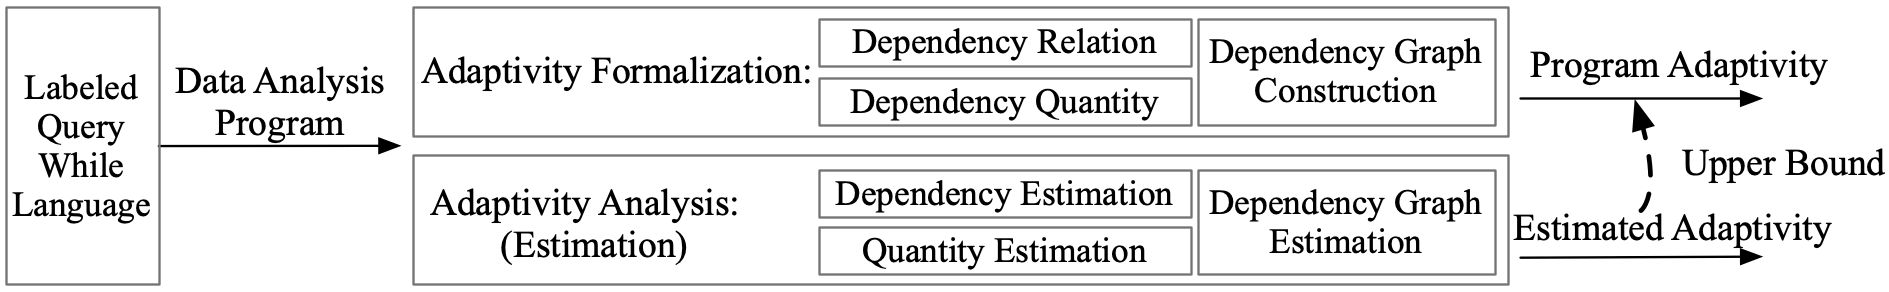
\includegraphics[width=1.0\textwidth]{architecture.png}
%     \vspace{-0.8cm}
%   \caption{High level architecture}
%     \label{fig:structure}
%     \vspace{-0.6cm}
% \end{figure}

\subsubsection{Static analysis}
%%%%%%%%%%%%%%%%%%%%%%%%%%%%%%% Previous Version Below that might be useful when make passes %%%%%%%%%%%%%%%%%
%  \detailed{The definition of adaptivity comes from the aforementioned execution-based dependency graph, 
%  our static analysis statically provides a sound upper bound on this adaptivity, via constructing another weighted graph, we call it estimated dependency graph. The upper bound is then found by searching a sound path with respect to our adaptivity in the generated graph. Different from the execution-based dependency which needs the trace from the execution, estimated one is built by our static analysis algorithm which takes the program itself as input. In brief, our algorithm is consist of a graph-generation algorithm, a weight computation algorithm and finally a path searching algorithm in the generated weighted graph.
%  }
%%%%%%%%%%%%%%%%%%%%%%%%%%%%%%% Previous Version Below that might be useful when make passes %%%%%%%%%%%%%%%%%
% \todo{In order to have a sound and accurate upper bound on the  adaptivity of a program $c$,
% we design a program analysis framework named {\THESYSTEM}.
% This framework composes two algorithms as shown in the double-stroke box and the dashed box in Fig.~\ref{fig:adaptfun}.
% The first algorithm in the double-stroke box combines the quantitative and dependency analysis techniques.
% It produces an estimated \emph{dependency graph} for a program.
% The second algorithm in the dashed box is a walk length estimation algorithm.
% It computes the upper bound on the program's \emph{adaptivity} over the estimated graph.}
% \jl{Since the definition of adaptivity comes from the aforementioned execution-based dependency graph, 
%  our static analysis statically provides a sound upper bound on this adaptivity via approximating this graph. The estimated graph is called \emph{estimated dependency graph}. 
%  The upper bound is then computed by searching the walk in this graph such that it can give a sound bound on the adaptivity.
%  Different from the execution-based dependency graph, the estimated one is produced by our static anlaysis algorithm, which only takes the program as input and does not rely on the execution history.
%  In brief, our algorithm is consist of a weighted graph-generation algorithm and a adaptivity computation algorithm over the graph.
%  }

 %%%%%%%%%%%%%%%%%%%%%%%%%%%%%%% Previous Version Above for Reference  %%%%%%%%%%%%%%%%%
To compute statically a sound and accurate upper bound on the \emph{adaptivity} of a program $c$,
we design a program analysis framework named {\THESYSTEM} (formally in Section \ref{sec:algorithm}). 
The structure of {\THESYSTEM} (Fig.~\ref{fig:adaptfun}) reflects in part the definition of adaptivity we discussed. Specifically, {\THESYSTEM} is composed by two algorithms (the ones in dashed boxes in the figure), one for building a dependency graph, called \emph{estimated dependency graph}, and the other to estimate the adaptivity from this graph.  
The first algorithm generates the \emph{estimated dependency graph} using several program analysis techniques. Specifically,
 {\THESYSTEM} extracts the vertices and the query annotations by looking at the assigned variables of the program, it estimates the edges by using control flow and data flow analysis, and it estimates the weights by using symbolic reachability-bound analysis---weights in this graph are symbolic expressions over input variables. 
% This combined analysis allow us to obtain more accurate upper bounds than what we would obtain by using any of these single analysis technique in isolation.
The second algorithm estimates the
% longest 
walk which respects the weights and which visits the maximal number of query vertices.
%  as possible. 
The two algorithms together gives us an  upper bound on the program's \emph{adaptivity}.

 \begin{figure}
  \centering    
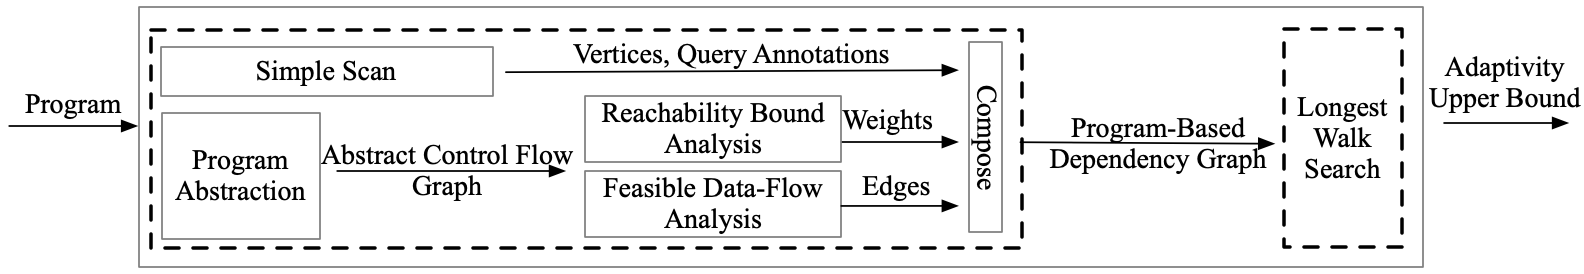
\includegraphics[width=1.0\columnwidth]{adapfun.png}
  \vspace{-0.8cm}
  \caption{The overview of {\THESYSTEM}}
  \label{fig:adaptfun}
  \vspace{-0.5cm}
\end{figure}

 
%%%%%%%%%%%%%%%%%%%%%%%%%%%%%%%%%%% Details Below that might be useful when others are making passes %%%%%%%%%%%%%%%%%
%   \detailed{Fig.~\ref{fig:overview-example}(c) is the resulting estimated graph of our static analysis algorithm which consumes the program in Fig.~\ref{fig:overview-example}(a).The edges are generated by our graph generation algorithm which combines control flow analysis and data flow analysis, presented in Section~\ref{sec:alg_edgegen}). We can easily see the generated graph in Fig.~\ref{fig:overview-example}(c) is a safe approximation of its execution-based counterpart in Fig.~\ref{fig:overview-example}(b), in the way that we can find a corresponding edge in Fig.~\ref{fig:overview-example}(c) for all the edges in Fig.~\ref{fig:overview-example}(b). We call the weight of every vertex computed by our algorithm as estimated weight,  }
%   estimated by using a reachability-bound estimation algorithm (presented in Section~\ref{sec:alg_weightgen}). \detailed{Different from the execution-based weight $w_1$ or $w_k$ in Fig.~\ref{fig:overview-example}(b) which is a function whose output relies on the initial trace, our estimated weight} can be symbolic and provide a sound upper bound on its execution-based weight of the corresponding vertex in the execution-based dependency graph. For instance, 
%   the estimated weight $k$ of the vertex $x^{3}$ in Fig.~\ref{fig:overview-example}(c) is a sound upper bound on the execution-based weight $w_k$ of vertex $x^{3}$ in Fig.~\ref{fig:overview-example}(b), with the same starting trace $\trace$, $w_k(\trace) \leq\trace(k)$. $\trace(k)$ means getting the value of variable $k$ in the trace $\trace$. The soundness of this step is proved in Theorem~\ref{thm:addweight_soundness}.   
%
We show in Fig.~\ref{fig:overview-example}(c) the estimated dependency graph that our static analysis algorithm returns for the program $\kw{twoRounds(k)}$ in Fig.~\ref{fig:overview-example}(a).
Vertices and query annotations are the same as the ones in Fig.~\ref{fig:overview-example}(b), simply inferred by scanning the program.
 Every edge in Fig.~\ref{fig:overview-example}(b) is precisely inferred by our combined data flow and control flow analysis, this is why Fig.~\ref{fig:overview-example}(c) contains exactly the same edges.
The weight of every vertex is computed using a reachability-bound estimation algorithm which outputs a symbolic expression over the input variables, representing an upper bound on the number of times each assignment is executed.
% \wq{symbolic and provide a sound upper bound on its execution-based weight of the corresponding vertex in the execution-based dependency graph.
% $w_k(\trace) \leq \trace(k)$. $\trace(k)$ means getting the value of variable $k$ in the trace $\trace$. The soundness of this step is proved in Theorem~\ref{thm:addweight_soundness}.}
For example, consider the vertex $x^{3}$, its weight is $k$ and this provides an upper bound on the value returned by the weight function \DIFdelbegin \DIFdel{$\lambda \trace. \rho(\trace)k$ }\DIFdelend \DIFaddbegin \highlight{$\kw{lastVal}(\trace,k)$} \DIFaddend associated with vertex $x^{3}$ in Fig.~\ref{fig:overview-example}(b) for any initial state. 
% Indeed, 
% for any initial trace $\trace_0$, when $w_{x^{3}}(\trace_0)$ executes the program and counts the
% execution times of command $3$,
% we expect that this counts is at most the the loop iterations, i.e. $k$'s initial value from $\trace_0$.

The algorithm searching for the walk first finds a path $l^6:{}^1_1 \to a^5: {}^k_0 \to x^3: {}^k_1$, and then constructs a walk based on this path. Every vertex on this walk is visited once, and the number of vertices with query annotation $1$ in this walk is $2$, which is the upper bound we expect.
{It is worth noting here that $x^3$ and $a^5$ can only be visited once because there isn't an edge to go back to them, even though they both have the weight $k$}.  So the algorithm $\pathsearch$ computes the upper bound $2$ instead of $2k+1$. Note that $2$ is not always tight, for example when $k = 0$.
% In this sense, instead of simply computing the weighted length of this path ($2k+1$) as adaptivity, the algorithm $\pathsearch$ computes the upper bound $2$. Note that $2$ is not always tight, for example when $k = 0$.
% \todo{Can you double check if this is clear?}
% \mg{I think we should add a sentence to say that this bound is actually not always tight.}
\DIFaddbegin 

\DIFaddend %%%%%%%%%%%%%%%%%%%%%%%%%%%%%%%%%%%%%%%%%%% Language %%%%%%%%%%%%%%%%%%%%%%%%%%%%%%%%%%%%%%%%%%%
\section{Labeled Query  While  Language}
\label{sec:loop_language}
The language of {\THESYSTEM} is a standard while language with labels to identify different components and with primitives for queries, and equipped with a  trace-based operational semantics which is the main technical tool we will use to define the program's adaptivity.

%\subsection{Syntax}
%\label{sec:syntax}
\vspace{-0.1cm}
{\small
\[
\begin{array}{llll}
\mbox{Arithmetic Expression} 
& \aexpr & ::= & 
n ~|~ {x} ~|~ \aexpr \oplus_a \aexpr 
~|~ \elog \aexpr  ~|~ \esign \aexpr ~|~ \max(a, a) ~|~ \min(a, a)
\\
\mbox{Boolean Expression} & \bexpr & ::= & 
%
\etrue ~|~ \efalse  ~|~ \neg \bexpr
 ~|~ \bexpr \oplus_b \bexpr
%
~|~ \aexpr \sim \aexpr 
\\
%
\mbox{Expression} & \expr & ::= & v ~|~ \aexpr \sep \bexpr ~|~ [\expr, \dots, \expr]
\\  
%
\mbox{Value} 
& v & ::= & { n \sep \etrue \sep \efalse ~|~ [] ~|~ [v, \dots, v]}  
\\
%
\mbox{Query Expression} 
& {\qexpr} & ::= 
& { \qval ~|~ \aexpr ~|~ \qexpr \oplus_a \qexpr ~|~ \chi[\aexpr]} 
\\
%
\mbox{Query Value} & \qval & ::= 
& {n ~|~ \chi[n] ~|~ \qval \oplus_a  \qval ~|~ n \oplus_a  \chi[n]
    ~|~ \chi[n] \oplus_a  n}\\
\mbox{Label} 
& l & \in & \mathbb{N} \cup \{\lin, \lex\} \\
\mbox{Labeled Command} 
& {c} & ::= &   [\assign {{x}}{ {\expr}}]^{l} ~|~  [\assign {{x} } {{\query(\qexpr)}}]^{l}
~|~ {\ewhile [ \bexpr ]^{l} \edo {c} }
 \\
 &&&
~|~ {c};{c}  
~|~ \eif([\bexpr]{}^l , {c}, {c}) 
~|~ [\eskip]^l 
\end{array}
\]
\vspace{-0.1cm}
}

%%%%%%%%%%%%%%%%%%%%%%%%%%%%%%%%%%% Details on Explaining the Syntax and Operational Semantics,
%%%%%%%%%%%%%%%%%%%%%%%%%%%%%%%%%%% that might be useful when others are making passes %%%%%%%%%%%%%%%%%
% \wq{As we have seen in the $\kw{twoRounds(k)}$ example in Fig.~\ref{fig:overview-example}(a), a program is expressed by labeled commands $c$. Our language supports the composition of labeled commands $c;c$, $[skip]^l$, the if condition $\eif([\bexpr]^l, c, c)$, the while command $\ewhile [\bexpr]^l \edo {c} $. The label $l$ records the location of this command, as a nature number $\mathbb{N}$ indicating the line number. Besides, it can also be $in$ or $ex$, used for annotating input variables and results and will not show up in labeled commands.} \wqside{Is it true that in and ex will not appear in the l in command?} 
%
% The boolean condition $b$ of the if and while commands is a standard boolean expression, which covers {\tt true} or {\tt false}, basic boolean connectives such as logical and logical or denoted by $\oplus_b$, logical negation $\neg$, and also comparison between arithmetic expressions $a \sim a$,  where $\sim$ stands for the basic operations such as $\leq,=,<,$ etc.  The arithmetic expression $a$ can be a constant $n$ denoting integer, a variable $x$ from some countable variable set $\mathcal{VAR}$, binary operation $\oplus_a$ such as addition, product, subtraction, etc, over arithmetic expressions, log and sign operation, minimal and maximum of two arithmetic expressions. An expression $e$ is then either a standard arithmetic expression or a boolean expression, or a list of expressions.
%
% \wq{As a reminder, the vertices of either the execution-based or program-based graphs in Fig.~\ref{fig:overview-example}(b) or Fig.~\ref{fig:overview-example}(c) are assigned variables and these assigned variables come from our two assignment commands: the standard assignment $[\assign{x}{\expr}]^l$, and our main novelty, the query request assignment $[\assign{x}{q(\qexpr)}]^l$.  The query is specified by a query expression $\qexpr$, which contains the necessary information for a query request. The query expression can be either the normal form $\alpha$, or just an arithmetic expression $a$ to express constant queries, or $\chi[\aexpr]$ representing the values at a certain index $\aexpr$ in a row $\chi$ of the database. Besides, we also allow combined access to the database in query expressions by means of $\qexpr \oplus \qexpr$.} For example, $\chi[3] + 5$ represents a query which asks the value from the column 3 of each database raw $\chi$, adds 5 to each of these values, and then computes the average of these values.
% In reality, if a data analyst wants to ask a simple linear query which returns the first element of the row, they can simply use the command $ \assign{x}{q(\chi[1])}$ in their data analysis program.
Expressions include
standard arithmetic (with value $n \in \mathbb{N}\cup \{ \infty \}$) and boolean expression, ($\aexpr$ and $\bexpr$) and extended query expressions $\qexpr$.
A query expression $\qexpr$ can be either a simple arithmetic expression $a$, an expression of the form $\chi[\aexpr]$ where $\chi$ represents a row of the database  and  $\aexpr$ represents an index used to identify a specific attribute of the row $\chi$, a combination of two query expressions, $\qexpr \oplus_{a} \qexpr$, or a normal form $\qval$.
For example, the query expression $\chi[3] + 5$  denotes the computation that
obtains
the value in the $3$rd column of $\chi$ in one row and then adds $5$ to it.

Commands are the typical ones from while languages with an additional command $\assign{x}{\query(\qexpr)}$ for query requests which can be used to interrogate
 the database and compute the linear query corresponding to $\qexpr$.
Each command is annotated with a label $l$, \DIFaddbegin \DIFadd{and }\DIFaddend we will use natural numbers as labels to record
the location of each command, so that we can uniquely identify them.
We also have a set \DIFaddbegin \DIFadd{of labels $\ldom$, a set }\DIFaddend $\mathcal{LV}$  of labeled variables (simply variables with a label), \DIFaddbegin \DIFadd{and }\DIFaddend a set $\cdom$ of all the programs.
We denote by $\mathbb{LV}(c)$ the set of labeled variables assigned in an assignment command in the program $c$.  
We denote by  $\qvar(c)$ the set of labeled variables that are assigned the result of a query in the program $c$.
 \DIFaddbegin \highlight{We provide the table of notations in Table~\ref{tb:notation} for quick reference.}
\DIFaddend 

% \mg{Please double check this notation.}


% In this the command, the query expression $\qexpr$ is sent to the database server as a request.
% Then the server will compute the average value of $\qexpr$ over each row of the hidden database $\chi$ and return us the result.
% For instance, when we execute the command $\assign{x}{\query(\chi[3] + 5)}$,
% the server will receive query request in form of $\chi[3] + 5$,
% then compute the average value of $\chi[3] + 5$ over each raw of $\chi$, and return the result to us. 
% The server is used as external API for computing the results over the hidden database $\chi$.

\subsection{ Trace-based Operational Semantics}
%DIF <   \wq{Our operational semantics uses the trace $\trace \in \mathcal{T}$ to track the history of the program execution, we use $\mathcal{T} $ for the set of traces. To be precise, the trace is a list of events and an event tracks the useful information about one step of the evaluation. When a program $c$ is evaluated in our operational semantics$\config{c, \trace} \to \config{c', \trace'} $, it starts with an initial trace $\trace$, evaluates to $c'$ , and along with the program evaluation, events are collected in the evaluation order and appended to $\trace$, and then we get the result trace $\trace'$. We can easily get the history of the evaluation of the program $c$ by looking at these newly added events in $\trace$ with respect to the initial trace $\trace$.  }

%DIF >   \wq{Our operational semantics uses the trace $\trace \in \mathcal{T}$ to track the history of the program execution, we use $\mathcal{T} $ for the set of traces. To be precise, the trace is a list of events and an event tracks the useful information about one step of the evaluation. When a program $c$ is evaluated in our operational semantics$\config{c, \trace} \to \config{c', \trace'} $, it starts with an initial trace $\trace$, evaluates to $c'$ , and along with the program evaluation, events are collected in the evaluation order and appended to $\trace$, and then we get the result trace $\trace'$. We can easily get the history of the evaluation of the program $c$ by looking at these newly added events in $\trace$ with respect to the initial trace $\trace$.  }
%DIF >  \highlight{Comment: A lot of notation is provided in section 3.1, some standard and some less-so. A table to summarize would be helpful for the reader to orient themselves during the rest of the paper. On a minor note: the combine operator (::) is used only once (in figure 5) which the concat operator (++) is used everywhere else (e.g., definitions 2 and 4) with singleton traces.}
We use a trace-based operational semantics tracking the history of program execution. The operational semantics is parameterized by a database that can be accessed only through queries. Since this database is fixed, we omit it from the semantics but it is important to keep in mind that this database exists and it is what allows us to evaluate queries.
A \emph{trace}
$\trace$ is a list of \emph{events} generated when executing specific commands. We denote by $\mathcal{T}$ the set of traces and we will use list notation for traces,
 where $[]$ is the empty trace, the operator $\traceadd$ combines an event and a trace in a new \DIFdelbegin \DIFdel{event}\DIFdelend \DIFaddbegin \DIFadd{trace}\DIFaddend , 
and the operator $\tracecat$ concatenates two traces. 
We have two kinds of events: \emph{assignment events} and \emph{testing events}. 
Each event consists of a quadruple,
and we use $\eventset^{\asn}$ and $\eventset^{\test}$ to denote the set of all assignment events and testing events, respectively.
% \begin{center}
% $ \begin{array}{lllll}
% \mbox{Event} 
% & \event & ::= & 
% {({x}, l, v, \bullet)} ~|~ { ({x}, l, v, \qval)}  ~|~{(\bexpr, l, v, \bullet)}  
% \\
% \end{array}$
% \end{center}
\begin{center}
  $ \begin{array}{lllll}
  \mbox{Event} 
  & \event & ::= & 
  ({x}, l, v, \bullet) ~|~ ({x}, l, v, \qval)  & \mbox{Assignment Event} \\
  &&& ~|~(\bexpr, l, v, \bullet)  & \mbox{Testing Event}
  \\
  \end{array}$
  \end{center}
An assignment event tracks the execution of an assignment  or a query request and consists of the assigned variable, the label of the command that generates it, the value assigned to the variable, and the normal form  $\qval$ of the query expression that has been requested, if this command is a query request, otherwise a default value $\bullet$.
A testing event tracks the execution of an if or while command and consists of the guard of the command, the label, the result of evaluating the guard, the last element $\bullet$. 
 We use the operator $\env (\trace) x$ to fetch the latest value assigned to  $x$ in the trace $\trace$, the operator
$\vcounter$ to count the occurrence of a labeled variable in the trace. \DIFaddbegin \highlight{ The function $\kw{lastVal}(\tau, x)$ mentioned in Section~\ref{sec:adaptivity-informal} can be 
expressed as $\lambda \trace. \env (\trace) x$. For any initial trace $\trace$, $\kw{lastVal}(\tau, x)$ returns the latest value of $x$ in $\trace$.
}
\DIFaddend We denote by $\tlabel(\trace) \subseteq \ldom$ the set of the labels occurring in $\trace$.
Finally, we use $\mathcal{T}_0(c) \subseteq \mathcal{T}$ to denote the set of \emph{initial traces}, the ones
which assign a value to the input variables. We use $\eventset$ to denote the set of all events.


The trace-based operational semantics is described in terms of a small step evaluation relation
$\config{c, \trace} \to \config{c', \trace}'$  describing how a configuration program-trace evaluates to another
configuration program-state. \DIFdelbegin \DIFdel{The rules for the operational semantics are described }\DIFdelend \DIFaddbegin \DIFadd{Selected rules are shown }\DIFaddend in Fig.~\ref{fig:os}.
The rules for assignment and query generate assignment events, while the rules for while and if generate testing events. 
\DIFdelbegin \DIFdel{The rules for the standard while language constructs correspond to the usual rules extended to deal with traces. 
}\DIFdelend We have relations $\config{\trace, \expr} \earrow v $  and $\config{\trace, \bexpr} \barrow v $  to evaluate expressions and boolean expressions, respectively. 
\DIFdelbegin \DIFdel{Their definitions are in the supplementary material.
}\DIFdelend %   \mg{Can you please confirm that this is true?} Yes
The only rule that is non-standard is the $\textbf{query}$ rule. When evaluating a query, the query expression $\qexpr$ is first simplified to its normal form $\alpha$ using an evaluation relation $\config{\trace, \qexpr} \qarrow \qval$. 
\DIFdelbegin \DIFdel{Then }\DIFdelend \DIFaddbegin \DIFadd{The }\DIFaddend normal form $\qval$ characterizes the linear query that is run against the database. The query result $v$ is the expected value of the function $\lambda \chi.\qval$ applied to each row of the dataset. We summarize this process with the notation $\query(\qval) = v$ in the rule $\textbf{query}$. 
Once the answer of the query is computed, the rules record all the needed information in the trace.  We will use $\to^*$ for the reflexive and transitive closure of $\to$. 
%%%%%%%%%%%%%%%%%%%%%%%%%%%%%%%%%%% The Detailed Version in Explaining the Event %%%%%%%%%%%%%%%%%%%%%%%%%%%%%%%%%%%%%%%%%%%%%%%%%
% First of all, as the key component of the program evaluation history, an event $\event$ stores necessary information on the evaluation results of commands. Depending on the types of commands, there are two kinds of events: the assignment event which is generated in the standard assignment and query request assignment commands, and the testing event which is generated in an if or while command. Both assignment and testing events are quadruples, but store different contents. 
%\jl{
% The key component of the program evaluation history is the event $\event$,
% which stores necessary information on the evaluation results of commands.
%%%%%%%%%%%%%%%%%%%%%%%%%%%%%%%%%%% The Detailed Version in Explaining the Assignment evaluation %%%%%%%%%%%%%%%%%%%%%%%%%%%%%%%%%%%%%%%%%%%%%%%%%
% The assignment event 
% targets the assignment so it needs to maintain the mapping between labeled assigning variable and the result assigned, to this end, the first three elements of the quadruple of an assignment event are the variable, the label, and the result $v$ of the assigned expression. Look at the rule $\textbf{assn}$ and rule $\textbf{query}$ in Fig.~\ref{fig:os}, the result $v$ is different: in the standard assignment, $v$ is the evaluation result of the assigned expression $e$ by the standard expression evaluation $\config{\trace, \expr} \earrow v $; in the query request assignment, the query expression $\qexpr$ is evaluated to its normal form $\alpha$ by the query expression evaluation $\config{\trace, \qexpr} 
% \qarrow \qval$ and is sent to a hidden mechanism, $query(\alpha) = v$ means that the return result of this query represented by $\alpha$ from the mechanism is $v$. Another difference of the generated assignment events in these two rules lands in the last element of the quadruple, which stores the query information. In the rule $\textbf{query}$, the fourth element is the query normal form $\alpha$ which is sent to the mechanism, while in the standard assignment rule $\textbf{assn}$, we use $\bullet$ to show this event is not directly related to a query request.
% \jl{The assignment event is generated when evaluating an assignment command or query request. It stores the value assigned to each variable and tracks the query request.
% The first three elements are the variable, the label of this command, and the value assigned to this variable.
% The forth element is the normal form of a query expression, $\qval$ if this command is a query request, otherwise a default value $\bullet$.
% As in rule $\textbf{assn}$ and rule $\textbf{query}$ in Fig.~\ref{fig:os}.
% When evaluating a query request, the query expression $\qexpr$ is first simplified to its normal form $\alpha$ by the evaluation rule $\config{\trace, \qexpr} \qarrow \qval$. 
% Then $\qval$ is sent to the hidden database on unknown server, which computes the query result and send back to us.
% This computation process is simplified into $\query(\qval) = v$ in the rule $\textbf{query}$.
% }
%%%%%%%%%%%%%%%%%%%%%%%%%%%%%%%%%%% The Detailed Version in Explaining the Expression Evaluation %%%%%%%%%%%%%%%%%%%%%%%%%%%%%%%%%%%%%%%%%%%%%%%%%
% \detailed{
% The expression evaluation $\config{\trace, \expr} \earrow v $ relies on the evaluation of arithmetic expressions $\config{\trace,\aexpr} \aarrow v $ and boolean expressions $\config{\trace, \bexpr} \barrow v $, they are standard and we leave The full rules in the appendix. The evaluation rules of query expressions are presented below.}
The query expression evaluation relation  $\config{\trace, \qexpr} \qarrow \qval$ is defined by the following rules which reduce a query expression to its normal form.
{\small
\begin{mathpar}
\inferrule{ 
  \config{\trace, \aexpr} \aarrow n
}{
 \config{\trace,  \aexpr} 
 \qarrow n
}
\and
\inferrule{ 
  \config{\trace, \qexpr_1} \qarrow \qval_1
  \and
  \config{\trace, \qexpr_2} \qarrow \qval_2
}{
 \config{\trace,  \qexpr_1 \oplus_a \qexpr_2} 
 \qarrow \qval_1 \oplus_a \qval_2
}
\and
\inferrule{ 
  \config{\trace, \aexpr} \aarrow n
}{
 \config{\trace, \chi[\aexpr]} \qarrow \chi[n]
}
\and
\inferrule{ 
  \empty
}{
 \config{\trace,  \qval} 
 \qarrow \qval
}
 \end{mathpar}
 }
%%%%%%%%%%%%%%%%%%%%%%%%%%%%%%%%%%% The Detailed Version in Explaining the Testing Event %%%%%%%%%%%%%%%%%%%%%%%%%%%%%%%%%%%%%%%%%%%%%%%%%
% The testing event is generated when evaluating if and while commands. To record the control flow information, the first element of the event is the guard $b$ in both if and while rules $\textbf{if-t,if-f}$ and rule $\textbf{while-t, while-f}$. The third element then stores the evaluation results of this guard, either true or false. Since the guard can not be a query request, the last element is $\bullet$. 
%%%%%%%%%%%%%%%%%%%%%%%%%%%%%%%%%%% The Details for The If and While Evaluation %%%%%%%%%%%%%%%%%%%%%%%%%%%%%%%%%%%%%%%%%%%%%%%%%
% \detailed{The rules for if hand while both have two versions, when the guard evaluates to true and false, respectively. In these rules, the evaluation of the guard also generates testing event and our trace is updated as well. }
% The rules for if and while both have two versions, 
% when the boolean expressions in the guards are evaluated to true and false, respectively. 
% In these rules, the evaluation of the guard generates a testing event and the trace is updated as well by appending this event.
% The rule $\textbf{query}$ evaluates the argument of a query request to a normal form and obtain the answer $v_q$ of the query $\query(v)$ from the mechanism. 
% Then the trace expanded by appending the query expression $\query(v)$ with the current annotation $(l,w)$. 
% The rule for assignment is standard and the trace remains unchanged. The sequence rule keeps tracking the modification of the trace, and the evaluation rule for if conditional 

%By the operational semantics rules, we prove no rule will shrink the trace in Appendix.
{\footnotesize %
\begin{figure}
\begin{mathpar}
\boxed{
\mbox{Command $\times$ Trace}
\xrightarrow{}
\mbox{Command $\times$ Trace}
}
\and
\boxed{\config{{c, \trace}}
\xrightarrow{} 
\config{{c',  \trace'}}
}
\\
\inferrule
{
\config{\trace, \expr} \earrow v 
\and
\event = ({x}, l, v, \bullet)
}
{
\config{[\assign{{x}}{\expr}]^{l},  \trace } 
\xrightarrow{} 
\config{\clabel{\eskip}^l, \trace \traceadd \event}
}
~\textbf{assn}
%
\and
%DIF < 
\DIFaddbeginFL 

\DIFaddendFL {
\inferrule
{
 \trace, \qexpr \qarrow \qval
 \and 
\query(\qval) = v
\and 
\event = ({x}, l, v, \qval)
}
{
\config{{[\assign{x}{\query(\qexpr)}]^l, \trace}}
\xrightarrow{} 
\config{{\clabel{\eskip}^l,  \trace \traceadd \event} }
}
~\textbf{query}
}
%
\and
%
\inferrule
{
 \trace, b \barrow \etrue
 \and 
 \event = (b, l, \etrue, \bullet)
}
{
\config{{\ewhile [b]^{l} \edo c, \trace}}
\xrightarrow{} 
\DIFdelbeginFL %DIFDELCMD < \config{{
%DIFDELCMD < c; \ewhile [b]^{l} \edo c),
%DIFDELCMD < \trace \traceadd \event}}
%DIFDELCMD < %%%
\DIFdelendFL \DIFaddbeginFL \config{{
c; \ewhile [b]^{l} \edo c,
\trace \traceadd \event}}
\DIFaddendFL }
~\textbf{while-t}
%
%
\DIFdelbeginFL \DIFdelFL{\quad
%DIF < 
}%DIFDELCMD < \inferrule
%DIFDELCMD < {
%DIFDELCMD <  \trace%%%
\DIFdelFL{, b \barrow }%DIFDELCMD < \efalse
%DIFDELCMD <  \and 
%DIFDELCMD <  \event %%%
\DIFdelFL{= (b, l, }%DIFDELCMD < \efalse%%%
\DIFdelFL{, \bullet)
}%DIFDELCMD < }
%DIFDELCMD < {
%DIFDELCMD < \config{{\ewhile [b]^{l}, \edo c, \trace}}
%DIFDELCMD < %%%
\DIFdelFL{\xrightarrow{} 
}%DIFDELCMD < \config{{
%DIFDELCMD <   \clabel{\eskip}^l,
%DIFDELCMD < \trace \traceadd \event}}
%DIFDELCMD < }
%DIFDELCMD < %%%
\DIFdelFL{~}\textbf{\DIFdelFL{while-f}}
%DIFAUXCMD
%DIF < 
%DIF < 
%DIFDELCMD < \and
%DIFDELCMD < \inferrule
%DIFDELCMD < {
%DIFDELCMD < \config{{c_1, \trace}}
%DIFDELCMD < %%%
\DIFdelFL{\xrightarrow{}
}%DIFDELCMD < \config{{c_1',  \trace'}}
%DIFDELCMD < }
%DIFDELCMD < {
%DIFDELCMD < \config{{c_1; c_2, \trace}} 
%DIFDELCMD < %%%
\DIFdelFL{\xrightarrow{} 
}%DIFDELCMD < \config{{c_1'; c_2, \trace'}}
%DIFDELCMD < }
%DIFDELCMD < %%%
\DIFdelFL{~}\textbf{\DIFdelFL{seq1}}
%DIFAUXCMD
%DIFDELCMD < \and
%DIFDELCMD < \inferrule
%DIFDELCMD < {
%DIFDELCMD <   \config{{c_2, \trace}}
%DIFDELCMD <   %%%
\DIFdelFL{\xrightarrow{}
  }%DIFDELCMD < \config{{c_2',  \trace'}}
%DIFDELCMD < }
%DIFDELCMD < {
%DIFDELCMD < \config{{\clabel{\eskip}^l; c_2, \trace}} %%%
\DIFdelFL{\xrightarrow{} }%DIFDELCMD < \config{{ c_2', \trace'}}
%DIFDELCMD < }
%DIFDELCMD < %%%
\DIFdelFL{~}\textbf{\DIFdelFL{seq2}}
%DIFAUXCMD
\DIFdelFL{\quad
}%DIFDELCMD < \inferrule
%DIFDELCMD < {
%DIFDELCMD <  \trace%%%
\DIFdelFL{, b \barrow }%DIFDELCMD < \etrue \and \event %%%
\DIFdelFL{= (b, l, }%DIFDELCMD < \etrue%%%
\DIFdelFL{, \bullet)
}%DIFDELCMD < }
%DIFDELCMD < {
%DIFDELCMD <  \config{{
%DIFDELCMD < \eif([b]^{l}, c_1, c_2), 
%DIFDELCMD < \trace}}
%DIFDELCMD < %%%
\DIFdelFL{\xrightarrow{} 
}%DIFDELCMD < \config{{c_1, \trace \traceadd \event}}
%DIFDELCMD < }
%DIFDELCMD < %%%
\DIFdelFL{~}\textbf{\DIFdelFL{if-t}}
%DIFAUXCMD
\DIFdelendFL %DIF >  \quad
%DIF >  %
%DIF >  \inferrule
%DIF >  {
%DIF >   \trace, b \barrow \efalse
%  \and 
%DIF >   \event = (b, l, \efalse, \bullet)
%DIF >  }
%DIF >  {
%DIF >  \config{{\ewhile [b]^{l}, \edo c, \trace}}
%DIF >  \xrightarrow{} 
%DIF >  \config{{
%DIF >    \clabel{\eskip}^l,
%DIF >  \trace \traceadd \event}}
%DIF >  }
%DIF >  ~\textbf{while-f}
% %
%DIF >  %
%DIF >  \and
% \inferrule
% {
%DIF >  \config{{c_1, \trace}}
%DIF >  \xrightarrow{}
%DIF >  \config{{c_1',  \trace'}}
%DIF >  }
%DIF >  {
%DIF >  \config{{c_1; c_2, \trace}} 
%DIF >  \xrightarrow{} 
%DIF >  \config{{c_1'; c_2, \trace'}}
%DIF >  }
%DIF >  ~\textbf{seq1}
%DIF >  \and
%DIF >  \inferrule
%DIF >  {
%DIF >    \config{{c_2, \trace}}
%DIF >    \xrightarrow{}
%DIF >    \config{{c_2',  \trace'}}
%DIF >  }
%DIF >  {
%DIF >  \config{{\clabel{\eskip}^l; c_2, \trace}} \xrightarrow{} \config{{ c_2', \trace'}}
%DIF >  }
%DIF >  ~\textbf{seq2}
%DIF >  \quad
%DIF >  \inferrule
%DIF >  {
%DIF >   \trace, b \barrow \etrue \and \event = (b, l, \etrue, \bullet)
%DIF >  }
%DIF >  {
%DIF >   \config{{
%DIF >  \eif([b]^{l}, c_1, c_2), 
%DIF >  \trace}}
%DIF >  \xrightarrow{} 
%DIF >  \config{{c_1, \trace \traceadd \event}}
%DIF >  }
%DIF >  ~\textbf{if-t}
%DIF >  \and
%DIF >  %
%DIF >  \inferrule
%DIF >  {
%  \trace, b \barrow \efalse
%  \and 
%  \event = (b, l, \efalse, \bullet)
% }
% {
% \config{{\eif([b]^{l}, c_1, c_2), \trace}}
% \xrightarrow{} 
% \config{{c_2, \trace \traceadd \event}}
% }
\DIFdelbeginFL \DIFdelFL{~}\textbf{\DIFdelFL{if-f}}
%DIFAUXCMD
\DIFdelendFL %DIF >  ~\textbf{if-f}
\end{mathpar}
  \vspace{-0.5cm}
    \caption{Trace-based Operational Semantics for Language.}
    \label{fig:os}
  \DIFdelbeginFL %DIFDELCMD < \vspace{-0.9cm}
%DIFDELCMD < %%%
\DIFdelendFL \DIFaddbeginFL \vspace{-0.1cm}
\DIFaddendFL \end{figure}
}
\DIFaddbegin 

    \begin{table}
      \caption{\highlight{Table of Notations}}
      \label{tb:notation}
      \begin{center}
        \begin{tabular}{| c |c |c| c| }
          \hline 
          \DIFaddFL{$\mathcal{LV}$   }& \DIFaddFL{universe of labeled variables  }& \DIFaddFL{$\qvar(c)$ }& \DIFaddFL{labeled query variables in $c$}\\ 
          \DIFaddFL{$\cdom$  }& \DIFaddFL{set of all programs }&  \DIFaddFL{$\trace$ }&   \DIFaddFL{trace, a list of }\emph{\DIFaddFL{events}}\\  
          \DIFaddFL{$\mathcal{T}$  }&  \DIFaddFL{set of traces }&  \DIFaddFL{$\trace \traceadd \event$  }& \DIFaddFL{combine a trace and an event  }\\
          \DIFaddFL{$\ldom$ }& \DIFaddFL{set of labels  }& \DIFaddFL{$\trace \tracecat \trace'$ }&  \DIFaddFL{trace concatenation }\\
          \DIFaddFL{$\tlabel(\trace) $  }&\DIFaddFL{set of labels occurring in $\trace$  }&  \DIFaddFL{$ \env (\trace) x$  }& \DIFaddFL{fetch latest value of  $x$ in a given $\trace$ }\\
          \DIFaddFL{$\mathcal{T}_0(c) $ }&  \DIFaddFL{set of }\emph{\DIFaddFL{initial traces}} & \DIFaddFL{$\kw{lastVal} (\trace, x)$  }& \DIFaddFL{fetch latest value of  $x$ in any $\trace$}\\
          \DIFaddFL{$\mathbb{LV}(c)$  }& \DIFaddFL{labeled variables in $c$ }& \DIFaddFL{$\vcounter(\trace, x^i)$ }& \DIFaddFL{occurrence of $x^i$ in the trace $\trace$}\\
          \hline 
        \end{tabular}
        \end{center}
        \vspace{-0.3cm}
      \end{table}
\DIFaddend %%%%%%%%%%%%%%%%%%%%%%%%%%%%%%%%%%%%%%%%%%% Adaptivity %%%%%%%%%%%%%%%%%%%%%%%%%%%%%%%%%%%%%%%%%%% 
\section{Definition of Adaptivity}
\label{sec:adaptivity}
 In this section, we formally present the definition of adaptivity for a given program. We first define a dependency relation between program variables, then define a semantics-based dependency graph, and finally look at the walk visiting the maximal number of query vertices in this graph. 
 % We first present the construction of the semantics-based dependency graph before the introduction of the formal definition of adaptivity. 

\subsection{May-dependency between variables}
\label{sec:dep}
%%%%%%%%%%%%%%%%%%%%%%%%%%%%%%%%%%% The Detail Explanation of Variable May-Dependency and Motivation on How to define it %%%%%%%%%%%%%%%%%%%%%%%%%%%%%%%%%%%%%%%%%%%%%%%%%
% \wq{we think the query $\query(\chi[2])$ (assigned variable $y^3$) may depend on the query $\query(\chi[1]$ (assigned variable $x^1$). 
  %  but vulnerable to queries request protected by differential privacy mechanisms. In our loop language, a query $q(e)$ represents a query request to the database through a mechanism, which add random noise to protect the return results. In this setting, the results of one query will be randomized due to the noise attached by the mechanism which fails the first candidate because witnessing the results of one query can no longer tells whether the change of the results comes from another query or the change of noise of the differential privacy mechanism. For example, suppose we have a program $p$ which requests two simple queries $q_1()$ and $q_2()$ with no arguments as follows.
%   \[
%   c_1 =\assign{x}{\query(\chi[2])} ;\assign{y}{\query(\chi[3] + x)}.
%   \]
%  $ c = \assign{x}{\query(\chi[1])} ; \assign{y}{\query(\chi[2])}$,
%  and 
% Specifically, in the {\tt Query While} language, the query request is composed by two components: a symbol $\query$ representing a linear query type and 
% % an argument
% the query expression $\qexpr$ as an argument, 
% which represents the function specifying what the query asks. 
% From our perspective, $\query(\chi[1])$ is different from $\query(\chi[2]))$. Informally,  
%
% in this example: $c_1 = \assign{x}{\query(0)}; \assign{z}{\query(\chi[x])}$.
% This candidate definition works well 
% Nevertheless, the first definition fails to catch control dependency because it just monitors the changes to a query, but misses the appearance of the query when the answers of its previous queries change. For instance, it fails to handle $}
%       c_2 = \assign{x}{\query(\chi[1])} ; \eif( x > 2 , \assign{y}{\query(\chi[2])}, \eskip )
%   $, but the second definition can. However, it only considers the control dependency and misses the data dependency. This reminds us to define a \emph{may-dependency} relation between labeled variables by combining the two definitions to capture the two situations.
%  $ p = \assign{x}{\query(\chi[1])} ; \assign{y}{\query(\chi[2])}$. 
% This candidate definition works well with respect to data dependency. However, if fails to handle control dependency since it just monitors the changes to the answer of a query when the answer of previous queries returned change. The key point is that this query may also not be asked because of an analyst decision which depend on the answers of previous queries. An example of this situation is shown in program $p_1$ as follows.
% There are two possible situations that a query will be "affected" by previous queries' results,  
% either when the query expression directly uses the results of previous queries (data dependency), or when the control flow of the program with respect to a query (whether to ask this query or not) depends on the results of previous queries (control flow dependency). To this end, our assigned variable dependency definition has the following two cases.   
% {
% \begin{enumerate}
%     \item One variable may depend on a previous variable if and only if a change of the value assigned to the previous variable may also change the value assigned to the variable.
%     \item One variable may depend on a previous variable if and only if a change of the value assigned to the previous variable may also change the appearance of the assignment command to this variable 
%     % in\wq{during?} 
%     during execution.
% \end{enumerate}
% }
%
%  The first case captures the data dependency. 
% For instance, in a simple program $c_1 =[\assign{x}{\query(\chi[2])}]^1 ;[\assign{y}{\query(\chi[3] + x)}]^2$, we think $\query(\chi[3] + x)$ (variable $y^2$) may depend on the query $\query(\chi[2]))$ (variable $x^1$), because the equipped function of the former $\chi[3] + x$ may depend on the data stored in x assigned with the result of $\query(\chi[2]))$. From our perspective, $\query(\chi[1])$ is different from $\query(\chi[2]))$. The second case captures the control dependency, for instance, in the program $
%       c_2 = [\assign{x}{\query(\chi[1])}]^1 ; \eif( [x > 2]^2 , [\assign{y}{\query(\chi[2])}]^3, [\eskip]^4 )
%
% There are two possible situations that a query will be ``influenced'' by previous queries' results,
% where either the query request is changed when the results of previous queries are changed (data dependency),
% or the  query request is disappeared when the results of previous queries are changed (control dependency). In this sense, our formal dependency definition considers both the two cases:
We are interested in defining a notion of dependency between program variables since assigned variables are a good proxy to study dependencies between queries---we can recover query requests from variables associated with queries. We consider dependencies that can be generated by either data or control flow.
% as follows,
% \begin{enumerate}
For example, in the program 
\DIFdelbegin \DIFdel{$c_1 =[\assign{x}{\query(\chi[2])}]^1 ;[\assign{y}{\query(\chi[3] + x)}]^2$
}\DIFdelend \DIFaddbegin \[\DIFadd{c_1 =}[\DIFadd{\assign{x}{\query(\chi[2])}}]\DIFadd{^1 ;}[\DIFadd{\assign{y}{\query(\chi[3] + x)}}]\DIFadd{^2}\]
\DIFaddend the query $\query(\chi[3] + x)$  depends on the query $\query(\chi[2]))$ through a \emph{value dependency} via  $x^1$.
% ), because $\chi[3] + x$ may depend on the data stored in x assigned by the result of $\query(\chi[2]))$. 
% From our perspective, $\query(\chi[1])$ is different from $\query(\chi[2]))$.
% \\
% (2). One query may depend on a previous query if and only if a change of the value returned
%     to the previous query request may also change the appearance of this query quest.
%     This captures the control influence.
Conversely, in the program
\DIFdelbegin \DIFdel{$c_2 = [\assign{x}{\query(\chi[1])}]^1 ; \eif( [x > 2]^2 , [\assign{y}{\query(\chi[2])}]^3, [\eskip]^4 )$ 
}\DIFdelend \DIFaddbegin \[\DIFadd{c_2 = }[\DIFadd{\assign{x}{\query(\chi[1])}}]\DIFadd{^1 ; \eif( }[\DIFadd{x > 2}]\DIFadd{^2 , }[\DIFadd{\assign{y}{\query(\chi[2])}}]\DIFadd{^3, }[\DIFadd{\eskip}]\DIFadd{^4 )}\] 
\DIFaddend the query $\query(\chi[2])$  depends on the query $\query(\chi[1])$ via the \emph{control dependency} of the guard of the if command involving the labeled variable $x^1$.
% \end{enumerate}
% \\
% \\
% The first case captures the data dependency. 
% For instance, in a simple program $c_1 =[\assign{x}{\query(\chi[2])}]^1 ;[\assign{y}{\query(\chi[3] + x)}]^2$, we think $\query(\chi[3] + x)$ (variable $y^2$) may depend on the query $\query(\chi[2]))$ (variable $x^1$), because the equipped function of the former $\chi[3] + x$ may depend on the data stored in x assigned with the result of $\query(\chi[2]))$. From our perspective, $\query(\chi[1])$ is different from $\query(\chi[2]))$.
% \\
% The second case captures the control dependency.
% For instance, in the program
% $c_2 = [\assign{x}{\query(\chi[1])}]^1 ; \eif( [x > 2]^2 , [\assign{y}{\query(\chi[2])}]^3, [\eskip]^4 )$, 
% we think the query $\query(\chi[2])$ ( or the labeled variable $y^3$) may depend on the query $\query(\chi[1])$ (via the labeled variable $x^1$). 
% \jl{ 
% Since both \emph{influences} are passing through variables, we choose to define the \emph{may-dependency}
% relation over all labeled variables, and then recover the query requests from query-associated variables, $\qvar(c)$.
% It relies on formal observation of the \emph{influences} via events in Def.~\ref{def:diff} and the \emph{may-dependency} between events in Def.~\ref{def:event_dep}.
% }

To define dependency between program variables we will consider two events that are generated from the same command, hence they have the same variable name or boolean expression and label, but have either different values or different query expressions.
%DIF < % \highlight{we use $\eventset$ to denote the set of all events, $\cdom$ for a set of all the programs.}
\DIFdelbegin \DIFdel{This is captured by the following. 
}\DIFdelend 



\begin{defn}
\label{def:diff}
\DIFdelbegin \DIFdel{Two events $\event_1, \event_2 \in \eventset$ are in the relation $\diff(\event_1, \event_2)$, if and only if:
}\DIFdelend \DIFaddbegin \highlight{Two events $\event_1, \event_2 $ at the same location differ in their values,  if they are either, 
\begin{enumerate}
  \item  of the form $\event_1 = (x, l, v_1, \bullet)$ and $event_1 = (x, l, v_2, \bullet)$, for a common variable (or Boolean expression) $x$ and program location $l$, and $v_1 \neq v_2$.
  \item  or of the form $\event_1 = (x, l, v_1, q_1)$ and $\event_1 = (x, l, v_2, q_2)$, where $q_1 \neq \bullet, q_2 \neq \bullet,$ and $q_1 \neq_q q2$.
\end{enumerate}
We denote this as $\diff(\event_1, \event_2)$. This notation is defined formally as follows:}
\DIFaddend {\small
\begin{subequations}
\begin{align}
& \pi_1(\event_1) = \pi_1(\event_2) 
  \land  
  \pi_2(\event_1) = \pi_2(\event_2) \\
& \land  
  \big(
   (\pi_3(\event_1) \neq \pi_3(\event_2)
  \land 
  \pi_{4}(\event_1) = \pi_{4}(\event_2) = \bullet )
  \lor 
  (\pi_4(\event_1) \neq \bullet
  \land 
  \pi_4(\event_2) \neq \bullet
  \land 
  \pi_{4}(\event_1) \neq_q \pi_{4}(\event_2)) 
  \big)
\end{align}
\label{eq:diff}
\end{subequations}
}
where $\qexpr_1 =_{q} \qexpr_2$ denotes the semantics equivalence between query values\footnote{The formal definition is in the supplementary material},
and $\pi_i$ projects the $i$-th element from the quadruple of an event.
\end{defn}
\DIFdelbegin \DIFdel{It is worth stressing that in the definition above, if two events are both generated from query requests, we are not comparing the query answers (the third element of the tuple), but the query expressions (the fourth element of the tuple).
For example in the running program in Fig.~\ref{fig:overview-example}(a), given different inputs $k = 1$ and $k = 2$
both events $\event_1 = (x, 3, 0, \chi[0] \cdot \chi[1])$ and $\event_2 = (x, 3, 0, \chi[0] \cdot \chi[2])$ can be generated from query request
$\clabel{\assign{x}{\query(\chi[j] \cdot \chi[k])} }^{3}$.
Even though $\pi_3(\event_1) = \pi_3(\event_2)$, these two events }\DIFdelend \DIFaddbegin \highlight{In the above definiton, we use $\neq_q$ to show the inequality between two query expressions.}
%DIF >  It is worth stressing that in the definition above, if two events are both generated from query requests, we are not comparing the query answers (the third element of the tuple), but the query expressions (the fourth element of the tuple).
\highlight{For instance, in the running program in Fig.~\ref{fig:overview-example}(a), the query command at line $3$, $\clabel{\assign{x}{\query(\chi[j] \cdot \chi[k])} }^{3}$ 
generates two events $\event_1 = (x, 3, 0, \chi[0] \cdot \chi[1])$ and $\event_2 = (x, 3, 0, \chi[0] \cdot \chi[2])$ 
given different inputs $k = 1$ and $k = 2$. The two query expressions $\chi[0] \cdot \chi[1]$ and $\chi[0] \cdot \chi[2]$ represent two 
different query requests, one using attribute 0 and attribute 1, the other using attribute 0 and attribute 2. So, we have  $\chi[0] \cdot \chi[1] \neq_q \chi[0] \cdot \chi[2]$. 
}
\DIFadd{Even though the two events have the same query results($\pi_3(\event_1) = \pi_3(\event_2)$), they }\DIFaddend are still different by our definition.
%% \remove{The Equation~\ref{eq:diff}(b) captures this by first checking
%% $\pi_4(\event_1) \neq \bullet \land \pi_4(\event_2) \neq \bullet$ to guarantee
%% both events are from query requests.
%% Then we check again the forth element $\pi_4(\event_1) \neq_q \pi_4(\event_2)$ to guarantee
%% the two events come from different query requests.}

We can now define when an event \emph{may depend} on another one in Definition~\ref{def:event_dep}\footnote{We consider here dependencies between assignment events. This simplifies the definition and is enough for the stating the following definitions. The full definition is in the supplementary material.}.

There are several components in Definition~\ref{def:event_dep}. The part with label (2a) requires that $\event_1$ and $\event_1'$ differ in their values ($\diff(\event_1, \event_1')$).
The next two parts (2b) and (2c) capture the value dependency and control dependency, respectively.
As in the literature on non-interference, and following~\cite{Cousot19a}, we formulate these dependencies as relational properties, in terms of two different traces of execution. 
We force these two traces to differ by using the event $\event_1$ in one and $\event_1'$ in the other. 
For the value dependency we check whether the change also creates a change in the value of $\event_2$ or not. We additionally check that the two events we consider appear the same number of times in the two traces - this to make sure that if the events are generated by assignments in a loop, we consider the same iteration. 
For the control dependency we check whether the change of the value in the assignment of event $\event_1$ affects the occurrence of event $\event_2$ or not. 
For this we require the presence of a test event whose value is affected by the change in $\event_1$
in order to guarantee that the computation goes through a control flow guard.
Similarly to the previous condition, we additionally check that the two test events we consider appear the same number of times in the two traces.
% 
\DIFdelbegin %DIFDELCMD < 

%DIFDELCMD < %%%
\DIFdelend \begin{defn}[Event May-Dependency]
  \label{def:event_dep}
  \vspace{-0.1cm}
  \DIFdelbegin \DIFdel{An event $\event_2\in \eventset^{\asn}$ }\emph{\DIFdel{may-depend}} %DIFAUXCMD
\DIFdel{on an event $\event_1 \in \eventset^{\asn}$ in a program ${c}$ denoted
  $\eventdep(\event_1, \event_2, c)$, if and only if
  }\DIFdelend \DIFaddbegin \highlight{An assignment event $\event_2\in \eventset^{\asn}$ \emph{may-depend} on another assignment event $\event_1 \in \eventset^{\asn}$ in a program ${c}$ \highlight{with a witness trace $\trace$}, 
   if and only if there exists an assignment event $\event_1'$ with the same location as $\event_1$ and which differs in values, such that we have one of the following situations: 
  \begin{enumerate}
    \item replacing $\event_1$ with $\event_1'$ in the execution trace will trigger a new execution trace whose newly generated event $\event_2'$ has the same location as $\event_2$ but differs in value with respect to $\event_2$. This situation captures a data dependency.
    \item replacing $\event_1$ with $\event_1'$ in the execution trace will trigger a new execution trace in which a test event after $\event_1$ in the original trace is flipped. This situation captured the control dependency.
  \end{enumerate}
  We denote this relation as
  $\eventdep(\event_1, \event_2, \highlight{\trace}, c)$, and we define it formally as follows.}
  \DIFaddend \begin{subequations}
  {\small 
  \vspace{-0.1cm}
  \begin{align}
  &  
  \exists \trace, \trace_0, \trace_1, \trace' \in \mathcal{T},\event_1' \in \eventset^{\asn}, {c}_1, {c}_2  \in \cdom  \st \diff(\event_1, \event_1') \land \\
  & 
  \quad \DIFdelbegin \DIFdel{(}\DIFdelend \exists  \event_2' \in \eventset \st 
  \left(
  \begin{array}{ll}   
    & \config{{c}, \trace_0} \rightarrow^{*} 
    \config{{c}_1, \trace_1 \tracecat [\event_1]}  \rightarrow^{*} 
    \config{{c}_2,  \trace_1 \tracecat [\event_1] \tracecat \trace \tracecat [\event_2] } 
     \\ 
     \bigwedge &
     \config{{c}_1, \trace_1 \tracecat [\event_1']}  \rightarrow^{*}
      \config{{c}_2,  \trace_1 \tracecat[ \event_1'] \tracecat \trace' \tracecat [\event_2'] } 
    \\
    \bigwedge & 
    \diff(\event_2,\event_2' ) \land 
    \vcounter(\trace, \pi_2(\event_2))
    = 
    \vcounter(\trace', \pi_2(\event_2'))\\
    \end{array}
    \right)\\ 
    & 
    \quad
    \lor 
    \left(
    \begin{array}{l} 
    \exists \trace_3, \trace_3'  \in \mathcal{T}, \event_b \in \eventset^{\test} \st 
    \\
     \quad \config{{c}, \trace_0} \rightarrow^{*} \config{{c}_1, \trace_1 \tracecat [\event_1]}  \rightarrow^{*}
     \config{c_2,  \trace_1 \tracecat [\event_1] \tracecat
     \trace \tracecat [\event_b] \tracecat  \trace_3} 
  \\ \quad \land
  \config{{c}_1, \trace_1 \tracecat [\event_1']}  \rightarrow^{*} 
  \config{c_2,  \trace_1 \tracecat [\event_1'] \tracecat \trace' \tracecat [(\neg \event_b)] \tracecat \trace_3'} 
  \\
  \quad \land \tlabel({\trace_3}) \cap \tlabel({\trace_3'})
  = \emptyset
  \land \vcounter(\trace', \pi_2(\event_b)) = \vcounter(\trace, \pi_2(\event_b)) 
      \land \event_2 \in \trace_3
      \land \event_2 \not\in \trace_3'
    \end{array}
    \right)
  \DIFdelbegin \DIFdel{),
  }\DIFdelend \end{align}
  }
  \label{eq:eventdep}
  \end{subequations}
  \vspace{-0.3cm}
  % , $\event_2 \in \trace_3$ or $\event_2 \notin \trace_3$ denotes that $\event_2$ belongs to $\trace_3$ or not.
  \end{defn}

In the running example in Fig.~\ref{fig:overview-example}(b), given the initial trace $[ (k, \lin, 1, \bullet)]$,
the program execution generates an
event $\event_1 = (x, 3, v_1, \chi[0] \cdot \chi[1])$ for
$\clabel{\assign{x}{\query(\chi[j] \cdot \chi[k])} }^{3}$,
and another event
$\event_2 = (l, 6, v_2, \chi[1] \cdot v_1 )$ for
$\clabel{\assign{l}{\query(\chi[k] \cdot a)} }^{6}$.
To check a may-dependency, we replace $\event_1$ with another event $\event_1' = (x, 3, v_1', \chi[0] \cdot \chi[1])$
where $v_1 \neq v_1'$.
We then continue to execute the program. The $6^{th}$ command generates $\event_2 = (l, 3, v_2, \chi[1] \cdot v_1' )$.
Since $\pi_4(\event_2) \neq_1 \pi_4(\event_2')$, we have  $\diff(\event_2, \event_2')$ according to Definition~\ref{def:diff} and then the dependency relation $\eventdep(\event_1, \event_2, \kw{twoRounds(k)})$.


 The dependency relation to variables can be extended by considering all the assignment events generated during the program's execution. Notice two variables can be the same in the following definition, this allows us to capture self-dependencies.
 \begin{defn}[Variable May-Dependency]
  \label{def:var_dep}
  \vspace{-0.2cm}
 \DIFdelbegin \DIFdel{A variable ${x}_2^{l_2} \in \lvar(c)$  }\emph{\DIFdel{may-depend}} %DIFAUXCMD
\DIFdel{on the 
  variable ${x}_1^{l_1} \in \lvar(c)$ in a program ${c}$,
  %DIF < 
  $\vardep({x}_1^{l_1}, {x}_2^{l_2}, {c})$, if and only if
}\DIFdelend \DIFaddbegin \highlight{ A variable ${x}_2$ assigned at location $l_2$ of a program $c$  \emph{may-depend} on the 
  variable ${x}_1$ assigned at location $l_1$ in the program ${c}$, 
  if and only if there exist two assignment events $\event_1$ and $\event_2$ associated with ${x}_1^{l_1}$ and ${x}_2^{l_2}$ respectively, a witness trace $\trace$,
  and $\event_2$ \emph{may-depend} on $\event_1$ with this witness trace $\trace$ in this program $c$. We denote this relation as
  $\vardep({x}_1^{l_1}, {x}_2^{l_2}, {c})$ and we define it formally as follows. 
 } 
\DIFaddend \begin{center}
$
{\small   \begin{array}{l}
\exists \event_1, \event_2 \in \eventset^{\asn}, \trace \in \mathcal{T} \st
\pi_{1}{(\event_1)}^{\pi_{2}{(\event_1)}} = {x}_1^{l_1}
\land
\pi_{1}{(\event_2)}^{\pi_{2}{(\event_2)}} = {x}_2^{l_2}% \\ \quad 
\land 
\eventdep(\event_1, \event_2, \trace, c) 
  \end{array}
}%
$
\vspace{-0.2cm}
\end{center}
  \end{defn}
%Notice that in the definition above we can also have that the two variables are the same, this allows us to capture self-dependencies.

%Going back to the running example in Fig.~\ref{fig:overview-example}(a), we have already discussed how  $\event_1 = (x, 3, v_1, \chi[0] \cdot \chi[1])$ and $\event_2 = (l, 6, v_2, \chi[1] \cdot v_1 )$ are in the event may-dependency relation. Moreover, we have that $x^3$ and $l^6$ are in the variable may-dependency relation by Definition~\ref{def:var_dep}.

\subsection{Semantics-based Dependency Graph}
\label{sec:design_choice}
%%%%%%%%%%%%%%%%%%%%%%%%%%%%%%%%%%% The Detailed Version in Introducing The Dependency Graph %%%%%%%%%%%%%%%%%%%%%%%%%%%%%%%%%%%%%%%%%%%%%%%%%
% we formally define the semantics-based dependency graph as follows. There are some notations used in the definition. The labeled variables of a program $c$  
% is a subset of the labeled  variables $\mathcal{LV}$, denoted by $\lvar(c) \in \mathcal{P}(\mathcal{VAR} \times \mathcal{L}) \subseteq \mathcal{LV}$.
% \wq{I think LV(c) means all the labeled assigned variables, because in Fig.3.b, j2 is not in the graph so j2 is not in LV(tworounds), please verify. If so, maybe LV(c) is not a good name, people may think it means all the label variables, instead of just assigned ones.}
% The set of query-associated variables (in query request assignments) for a program $c$ is denoted as $\qvar(c)$, where $\qvar: \cdom \to 
% \mathcal{P}(\mathcal{LV})$. The set of initial traces of a program $c$ is a subset of the  trace universe $\trace$, in which every initial trace contains the value for all the input variables of $c$. For instance, the initial trace $\trace_0$ contains the value of input variable $k$ in the $\kw{twoRounds(k)}$ example.
\begin{defn}[Semantics-based Dependency Graph]
  \label{def:trace_graph}
  Given a program ${c}$,
  its \emph{semantics-based dependency graph} 
  $\traceG({c}) = (\traceV({c}), \traceE({c}), \traceW({c}), \traceF({c}))$ \DIFdelbegin \DIFdel{is defined }\DIFdelend \DIFaddbegin \highlight{consists of four components: vertices are all the 
  labelled variables in the program $c$; directed edges are pairs of vertices in the  may dependency relation; weights where the weight $w$ of a vertex $x^l$ 
  is a function which takes an initial trace $\trace_0$ as input and returns the number of times $x^l$ appears in the execution trace of the program $c$ when starting from $\trace_0$; query annotations where a query annotation on a vertex
  can be see as a flag indicating whether the command associated with the vertex is a query assignment or not.
  }
  \DIFadd{The formal definition is }\DIFaddend as follows,
  {\small
  \[
  \begin{array}{lll}
    \text{Vertices} &
    \traceV({c}) & := \left\{ 
    x^l
    ~ \middle\vert ~ x^l \in \lvar(c)
    \right\}
    \\
    \text{Directed Edges} &
    \traceE({c}) & := 
    \left\{ 
    (x^i, y^j) 
    ~ \middle\vert ~
    x^i, y^j \in \lvar(c) \land \vardep(x^i, y^j, c) 
    \right\}
    \\
    \text{Weights} &
    \traceW({c}) & := 
    \{ 
    (x^l, w) 
    ~ \vert ~ 
    w : \tdom_0(c) \to \mathbb{N}
    \land
    x^l \in \lvar(c) \land
    \forall \trace_0 \in \tdom_0(c), \trace' \in \tdom, l' \st
    \\ & & \qquad \qquad
    \config{{c}, \trace_0} \to^{*} 
    \config{\clabel{\eskip}^{l'}, \trace_0 \tracecat \trace'} 
    \land w(\trace_0) = \vcounter(\trace', l) \} 
     \\
    \text{Query Annotations} &
    \traceF({c}) & := 
  \left\{(x^l, n)  
  ~ \middle\vert ~
   x^l \in \lvar(c) \land
  (n = 1 \Leftrightarrow x^l \in \qvar(c))\land ( n = 0 \Leftrightarrow  x^l \notin \qvar(c))
  \right\}
  \end{array},
  \]
  A semantics-based dependency graph $\traceG({c})= (\traceV({c}), \traceE({c}), \traceW({c}), \traceF({c}))$ is \emph{well-formed} if and only if $ \{x^l \ |\ (x^l,w)\in \traceW({c})\} = \traceV({c}) $.
  }
  \end{defn}
We can now define the \emph{semantics-based dependency graph} of a program $c$ in Definition~\ref{def:trace_graph}. We want this graph to combine quantitative reachability information with dependency information. 
% For instance, the initial trace of $\kw{twoRounds(k)}$ example contains the initial value of the input variable $k$.

 Vertices and query annotations are just read out from the program $c$. We have an edge in $\traceE(c)$ if we have a may-dependency between two labeled variables in $c$.
% For the dependency graph of our running example in Fig.~\ref{fig:overview-example}(b),
% the subscript in vertices $x^3$ and $l^6$ is $1$ because they both come from query requests.
% There is a directed edge from $x^3$ and $l^6$ because we identify the variable may-dependency relation, $\dep(x^3, l^6, \kw{twoRounds(k)})$ according to Definition~\ref{def:var_dep}.
A weight function $w \in \traceW(c)$ is a function that for every starting trace $\trace_0 \in \mathcal{T}_0(c)$ 
gives the number of times the assignment of the corresponding vertex $x^l$ is visited. Notice that weight functions are total and with range $\mathbb{N}$. This means that if a program $c$ has some non-terminating behavior, the set $\traceW(c)$ will be empty. 
To rule out this situation, we consider as well-formed only graphs with a weight for every vertex. 
%\highlight{This is also because programs that have non-terminating behaviors do not have the intuitive adaptivity.}
%MG: I don't think this sentence is clear
In the rest of the paper we  implicitly consider only well-formed semantics-based dependency graphs. 

% Going back to the example in Fig.~\ref{fig:overview-example}(b), the vertices $a^0$, $j^1$ and $l^6$ have weight function $\lambda \trace \st 1$ because commands $0, 1$ and $6$ are executed only once, given any arbitrary initial trace.
% The vertices corresponding to commands inside the loop body have weight function $\lambda \trace \st \env(\trace) k$ because they  will be executed the same number of times as the loop iteration times.



  \subsection{Adaptivity of a Program}
  \label{sec:sematnic_adaptivity}
 This notion of adaptivity is formulated in terms of an initial trace, specifying the value of the input variables, and of the walk on the graph $\traceG({c})$ which has the largest number of query requests.

In Fig.~\ref{fig:overview-example}(b), $\lambda \trace_0 \st (l^6 \to x^3)$ is a walk with two vertices and where each vertex is visited only once. 
With the assumption that $k \geq 1$, $\lambda \trace_0 \st (l^6 \to {a^5 \to a^5 \to \ldots} \to x^3)$ is a walk where the vertex $a^5$ is visited $\env(\trace) k$ times.
However, $\lambda \trace_0 \st (l^6 \to a^5 \to x^3 \to x^3)$ is not a walk because there is no edge from $x^3$ to $x^3$.
%\underbrace{a^5 \to a^5 \to \ldots}_{\env(\trace) k} 
The formal \DIFdelbegin \DIFdel{defintion }\DIFdelend \DIFaddbegin \DIFadd{definition }\DIFaddend of a walk is the following:
\begin{defn}[Walk]
\label{def:finitewalk}
Given a well-formed program $c$ with its semantics-based dependency graph $\traceG({c}) = (\traceV, \traceE, \traceW, \traceF)$, a \emph{walk} $k$ is a function that maps an initial trace $\trace_0$ to a sequence of vertices $(v_1, \ldots, v_{n})$
for which there is a sequence of edges $(e_1 \ldots e_{n - 1})$  satisfying
\begin{itemize}
\item $e_i = (v_{i},v_{i + 1}) \in \traceE$ for every $1 \leq i < n$,
\item and $v_i$ appears in $(v_1, \ldots, v_{n})$ at most $w_i(\trace_0)$ times for every $v_i \in \traceV$ and $(v_i, w_i) \in \traceW$.  
\end{itemize}
% $k(\trace_0) = (v_1, \ldots, v_{n})$
% and w
We denote by $\walks(\traceG(c))$
the set of all the walks $k$ in $\traceG(c)$.
\end{defn} 
Because for the adaptivity
% is intuitively 
we are interested in the dependency between queries,
we calculate a special ``length'' of a walk, the \emph{query length},  by counting only the vertices
corresponding to queries.
\begin{defn}[Query Length]
\label{def:qlen}
Given 
the semantics-based dependency graph $\traceG({c})$ of a well-formed program $c$,
 and a \emph{walk} 
 $k \in \walks(\traceG(c))$, 
%  with vertex sequence $(v_1, \ldots, v_{n})$, 
the \emph{query length} of $k$ is a function $\qlen(k):\tdom_0(c) \to \mathbb{N}$ that 
given an initial trace $\trace_0\in \tdom_0(c)$ 
gives
the number of vertices that correspond to query variables in the vertex sequence of $k(\trace_0)$.
It is defined as follows.
\begin{center}
   $
  \qlen(k) = \lambda \trace_0 \st |\big( v \mid v \in (v_1, \ldots, v_{n}) \land (v, 1) \in \traceF(c) 
%   \land
%   k \in \walks(\traceG(c)) 
  \land k(\trace_0) = (v_1, \ldots, v_{n}) \big)|,
$
\end{center}
where the notation $| (\ldots) |$ gives the number of vertices in a sequence.
\end{defn}
% \todo{Referring the running example}

% Under the assumption that $k \geq 1$, both walks $\lambda \trace_0 \st (l^6 \to x^3)$ and  $\lambda \trace_0 \st (l^6 \to \underbrace{a^5 \to a^5 \to \ldots}_{\env(\trace) k} \to x^3)$ in Fig.~\ref{fig:overview-example}(b) have query length $\lambda\trace_0 \st 2$ because only
% vertices $x^3$ and $l^6$ come from query requests.

 We can now define the adaptivity of a well-formed program as follows.
\begin{defn}
    [Adaptivity of a Program]
    \label{def:trace_adapt}
    Given a well-formed program ${c}$, 
    its adaptivity $A(c)$ is a function 
    $A(c) : \tdom_0(c)\to \mathbb{N}$
    defined as follows.
\begin{center}
$
    A(c) = \lambda \trace_0 \st \max \big 
    \{ \qlen(k)(\trace_0) \mid k \in \walks(\traceG(c)) \big \} 
$
\end{center}
\end{defn}
% Again, we define the adaptivity by considering only well-formed semantics-based dependency graphs. In Fig.~\ref{fig:overview-example}(b), the two dotted edges represent a finite walk with maximal query length, since it contains the only two query requests.
%   Each query request can be visited at most once, and so the adaptivity of this program is $\lambda \trace_0  \st 2$.


%%%%%%%%%%%%%%%%%%%%%%%%%%%%%%%%%%%%%%%%%%% Adaptfun %%%%%%%%%%%%%%%%%%%%%%%%%%%%%%%%%%%%%%%%%%% 
\section{The Adaptivity Analysis Algorithm - {\THESYSTEM}}
\label{sec:algorithm}
In this section, we present our program analysis {\THESYSTEM} for
computing an upper bound on the \emph{adaptivity} of a given program
$c$.
%
%% \remove{The high level idea behind {\THESYSTEM} is to first build
%% an \emph{estimated dependency graph} \progG(c) of a program $c$
%% (Section~\ref{sec:alg_weightedgegen}) which overapproximates the
%% semantics-based dependency graph in two dimensions: it
%% overapproximates the dependencies between assigned variables (Section~\ref{sec:alg_edgegen}), and, it
%% overapproximates the weights (Section~\ref{sec:alg_weightgen}). Then, {\THESYSTEM} uses a custom algorithm to estimate the 
%% walk of maximal query length on this graph, providing in this way an upper bound on the adaptivity of the
%% program.} 
%\highlight{ 
 The high-level idea behind {\THESYSTEM} is the following:
  \begin{enumerate}
    \item construct
    an \emph{estimated program dependency graph} \progG(c) of a program $c$;
    \item use a reachability-bound algorithm to estimate the weight of every vertex in the graph;
    \item  use an algorithm, which we call AdaptBD, to estimate an upper bound on the number of queries in the walk over the weighted dependency graph that visits \DIFaddbegin \DIFadd{the }\DIFaddend most query vertices. %This in turns gives us an upper bound to the adaptivity. 
  \end{enumerate}
  The \emph{estimated dependency graph} overapproximates the
  semantics-based dependency graph in two dimensions: it
  overapproximates the dependencies between assigned variables (Section~\ref{sec:alg_edgegen}), and, it
  overapproximates the weights (Section~\ref{sec:alg_weightgen}). Thanks to this, 
 we prove the upper bound provided by AdaptBD is a sound upper bound
  over the semantic-based adaptivity in Definition~\ref{def:trace_adapt} in Theorem~\ref{thm:adaptalg_soundness}.  
%}

%
%%%%%%%%%%%%%%%%%%%%%%%%%%%%%%%%%%%%%%%%%%%%%%%%%%%%%%%%%%%%%%%%%%%%%%%%%%%%%%%%%%%%%%%%%%%%%%%%%%%%%%%%%%%%%%%%%%%%%%%%%%%%%%%%%%%%%%%%%%%%%%%%%%%%%%%%%%
%%%%%%%%%%%%%%%%%%%%%%%%%%%%%%%%%%%%%%%%%%%%%%%%%%%%%%%%%%%% Edge And Weight Analysis %%%%%%%%%%%%%%%%%%%%%%%%%%%%%%%%%%%%%%%%%%%%%%%%%%%%%%%%%%%%%%%%
%%%%%%%%%%%%%%%%%%%%%%%%%%%%%%%%%%%%%%%%%%%%%%%%%%%%%%%%%%%%%%%%%%%%%%%%%%%%%%%%%%%%%%%%%%%%%%%%%%%%%%%%%%%%%%%%%%%%%%%%%%%%%%%%%%%%%%%%%%%%%%%%%%%%%%%%%%
%
\subsection{Weighted Dependency Graph Construction}
Given a program $c$, the set of vertices $\progV(c)$ and query annotations $\progF(c)$ of the \emph{estimated dependency graph} can be computed by simply
scanning the program $c$. These sets can be computed precisely and correspond to
the same sets in the semantics-based dependency graph.
This means that $\progG(c)$ has the same underlying vertex structure as 
the semantics-based graph $\traceG(c)$. The differences will be in the sets of edges and weights. 





%% \remove{\subsection{Weight and Edge Estimation}}
%% \label{sec:alg_weightedgegen}
%% \remove{The set of edges $\progE(c)$ and the set of weights $\progW(c)$ of the estimated dependency graph are estimated through an analysis combining control flow, data flow, 
%% and loop bound analysis. These analyses are naturally described over an  \emph{Abstract Transition Graph} of the input program, which we describe next.}
%% %
%% %%%%%%%%%%%%%%%%%%%%%%%%%%%%%%%%%%%%%%%%%%%%%%%%%%%%%%%%%%%% Abstract Dependency Graph %%%%%%%%%%%%%%%%%%%%%%%%%%%%%%%%%%%%%%%%%%%%%%%%%%%%%%%%%%%%%%%%
%% %
%% \subsubsection{\remove{Abstract Transition Graph}}
%% \label{sec:abscfg}
%% %%%%%%%%%%%%%%%%%%%%%%%%%%%%%%%%%%%%%%%%%%%%%% Previous Version For Reference %%%%%%%%%%%%%%%%%%%%%%%%%%%%%%%%%%%%%%%%%%%%%%
%% % An \emph{Abstract Transition Graph}, $\absG(c)$ for a program $c$ is composed of
%% % a vertex set $\absV(c)$ and an edge set $\absE(c)$, $\absG(c) \triangleq (\absV(c), \absE(c))$.
%% % \\
%% % Every 
%% % vertex $l \in \absV(c)$ is the label of a labeled command in $c$, which is unique.
%% % \\
%% % Each edge $(l \xrightarrow{dc} l') \in \absE(c)$ is an abstract transition
%% % between two program points $l, l'$. 
%% % There is an edge from $l$ to $l'$ if and only if
%% % the command with label $l'$ can execute right after the execution of the command with label $l$.
%% % % if and only if there is a control flow between two program points.
%% % Each edge is annotated by a constraint $dc \in \dcdom^{\top}$, which is generated from the command with label $l$.
%% % This constraint describes the abstract execution of the command with $l$. 
%% % The edge set is constructed in three steps summarized as follows (with detail in Apdix.).
%% % \begin{enumerate}
%% %     \item Computing \textbf{constrains} over the expression for every program's labeled command,
%% %   which is used as the annotation of an edge.
%% %   Its domain $\dcdom^{\top}$ is composed of the \emph{Difference Constraints} $DC(\mathcal{VAR}  \cup \constdom)$, the \emph{Boolean Expressions} $\booldom$ and $\top$.
%% % %
%% % \begin{itemize}
%% % \item The difference constraints $DC(\mathcal{VAR}  \cup \constdom)$ is the set of all the inequality of
%% % form $x' \leq y + v$ where $x \in \mathcal{VAR} $, 
%% % $y \in \mathcal{VAR}$ and $v \in \constdom$.
%% % The \emph{Symbolic Constant} set $\constdom = \mathbb{N} \cup \inpvar \cup{\infty \cup{Q_m}}$
%% % is the set of natural numbers with $\infty$, the input variables, and a symbol $Q_m$ representing the abstract value of a query request.
%% % An inequality $x' \leq y + v$ describes that the value of $x$ in the current state is
%% % at most the value of $y$ in the previous state plus some constant $v$.
%% % When a difference constrain shows up as an edge annotation, $l \xrightarrow{x' \leq y + v} l'$,
%% % it denotes that
%% % the value of variable $x$
%% % after executing the command at $l$ is at most
%% % the value of variable $y$ plus $v$ before the execution.
%% % For every expression in each of the label command, it is computed in three steps via program abstraction method adopted from the Section~6 in \cite{sinn2017complexity}. 
%% % %
%% % \item The Boolean Expressions $b$ from the set $\booldom$.
%% % $b$ on an edge $l \xrightarrow{b} l'$ describes
%% % that after evaluating the guard with label $l$,
%% % $b$ holds and the command with label $l$ will execute right after.
%% % %
%% % \item The top constraint, $\top$ denotes true. It is preserved for $\eskip$ command.
%% % %
%% % \end{itemize}
%% %     \item \textbf{Initial and final state} computation step generates two sets for each labeled command in $c$. 
%% %   The initial state contains the
%% %   label where this command {starts} executing, 
%% %   and the final state is a set
%% %   that contains the constraint of this command
%% %   and the continuation labels after the execution of this command.
%% %  \item \textbf{abstract event} computation step generates a set of edges for the $c$, by computing the initial state and finial state interactively and recursively.
%% % \end{enumerate}
%% %%%%%%%%%%%%%%%%%%%%%%%%%%%%%%%%%%%%%%%%%%%%%% Previous Version Above %%%%%%%%%%%%%%%%%%%%%%%%%%%%%%%%%%%%%%%%%%%%%%
%% %
%% \remove{We say that we have a \emph{transition} from a program point $l$ to a
%% program point $l'$ if and only if the command with label $l'$ can
%% execute right after the execution of the command with label $l$.
%% The \emph{Abstract Transition Graph} $\absG(c)$ of a program $c$ is a
%% graph with the set of labels of program points in $c$  (including a 
%% label $\lex$ for the exit point) as the set of
%% vertices $\absV(c)$, and with the set of transitions in $c$ as the set of
%% edges $\absE(c)$. Each edge of the graph is annotated with either
%% the symbol $\top$, a boolean expression or a \emph{difference
%% constraint}~\cite{sinn2017complexity}.
%% A difference constraint is an inequality of the form $x' \leq y + v$ {or $x' \leq v$}
%% where $x, y$ are variables and $v \in \constdom$ is a symbolic
%% constant: either a natural number, the symbol $\infty$, an input
%% variable or a symbol $Q_m$ representing a query request.  We denote by
%% $\dcdom$ the set of difference constraints.
%% A difference constraint on an edge, $l \xrightarrow{x' \leq y + v}
%% l'$ {or $l \xrightarrow{x' \leq v} l'$}, denotes that after executing the command at location $l$ the
%% value of the variable $x$ is at most the value of the expression $y +
%% v$ {resp. $v$} before the execution of the command $l'$.
%% A boolean value $b$ on an
%% edge, $l \xrightarrow{b} l'$, denotes that after evaluating the guard
%% of an if or a while command with label $l$, $b$ holds and the next
%% command to be executed is the one with label $l'$.  A $\top$ symbol on
%% an edge, $l \xrightarrow{\top} l'$ denotes that the command with label
%% $l$ is a $\eskip$, {and the commands that do not interfere with any loop counter variable}.
%% We compute difference constraints and the other annotation via a
%% simple program abstraction method adopted
%% from \cite{sinn2017complexity}, described in details in the
%% supplementary material. }
%% % \mg{It would be good to have a simple short sketch.}
%% %\\
%% %% \jl{   
%% %% 2. Computing the \textbf{Initial and final state} for each labeled command in $c$. 
%% %%   The initial state contains the
%% %%   label where this command {starts} executing, 
%% %%   and the final state is a set
%% %%   that contains the constraint of this command
%% %%   and the continuation labels after this command.
%% %%   \\ 
%% %% %  \item 
%% %% 3. computing \textbf{abstract event}s and generating a set of edges for the $c$, by computing the initial state and finial state interactively and recursively.
%% %% %   Each edge is a pair of initial and finial state.
%% %% % \end{enumerate}
%% %% }

%% \remove{\textbf{Example.}
%% We show in Fig.~\ref{fig:abscfg_tworound}(b) the  abstract control flow graph,
%%  $\absG(\kw{twoRounds(k)})$ of the $\kw{twoRounds(k)}$ program we gave in 
%%   Fig.~\ref{fig:overview-example}(a) and which we also report in 
%%    Fig.~\ref{fig:abscfg_tworound}(a).}
%% % \mg{This example has many issues. First, many nodes do not respect the format that 
%% % we say difference constraint have. So, either we gave the wrong definition of difference constraints or we are being sloppy or we are using some shortening without telling it to the reader. In any case we need to fix this. Also, why one of the query is bound by $Q_m$ and the other one is instead bound by $k*a$? I think this example needs some serious reworking.}
%% % \jl{
%% % The edge $(1 \xrightarrow{j' \leq k} 2)$ on the top tells us the command 
%% % $\clabel{\assign{j}{k}}^1$ is executed with a continuation point $2$ such that the
%% % % where the 
%% % guard $\clabel{j > 0}^2$ will be evaluated next.
%% % The annotation $j' \leq k$ is a difference constraint 
%% % computed for
%% % % by abstracting
%% % the expression $k$ from the assignment command $\assign{j}{k}$.
%% % %  from the function $\absexpr(0)$.
%% % It represents that the value of $j$ is less than or equal to value of input variable $k$ after the
%% % execution of $\clabel{\assign{a}{0}}^0$ and before executing the loop.
%% % % Another example edge $5 \xrightarrow{a' \leq a + x } 2$ describes the execution of
%% % %  the command
%% % % $\clabel{\assign{a}{x + a}}^{5}$.
%% % The boolean constraint $j \leq 0 $ on the edge $2 \xrightarrow{j \leq 0} 6$
%% % represents the negation of the testing guard $j > 0$
%% % of the $\ewhile$ command with header at label $2$.
%% % }
%% % \mg{ The next sentence need a pass after we fix the example:
%% % The edge $(0 \xrightarrow{a' \leq 0} 1)$ on the top tells us the command 
%% % $\clabel{\assign{a}{0}}^0$ is executed with a continuation point $1$ such that the
%% % command $\clabel{\assign{j}{k}}^1$ will be executed next.
%% % % The annotation $a' \leq 0$ is a difference constraint 
%% % % computed for
%% % % the expression $0$ in the assignment command $\assign{a}{0}$.
%% % $a' \leq 0$ represents that the value of $a$ is less than or equal to $0$ after the
%% % execution of $\clabel{\assign{a}{0}}^0$ and before executing $\clabel{\assign{j}{k}}^1$.
%% % % Another example edge $5 \xrightarrow{a' \leq a + x } 2$ describes the execution of
%% % %  the command at line $5$
%% % % $\clabel{\assign{a}{x + a}}^{5}$.
%% % % This edge has difference constraint $a' \leq a+x $.
%% % % The $a'$ on the left side of $a' \leq a+x$ represents the value of $a$ after executing this assignment command.
%% % $j \leq 0 $ on the edge $2 \xrightarrow{j \leq 0} 6$
%% % represents the negation of the testing guard $j > 0$
%% % of the $\ewhile$ command with header at label $2$.
%% % The edge from $3$ to $4$ comes from the query request command $\clabel{\assign{x}{\query(\chi[j])} }^{3}$.
%% % The constraint over this edge, $x' < Q_m$ describes after executing $\assign{x}{\query(\chi[j])}$,
%% % % $\clabel{\assign{x}{\query(\chi[j])} }^{3}$, 
%% % the query request results stored in $x$ is bounded by $Q_m$. 
%% % }
%% The edge $(0 \xrightarrow{a' \leq 0} 1)$ on the top, tells us the command 
$\clabel{\assign{a}{0}}^0$ is executed with a continuation point $1$ such that the
% where the 
command $\clabel{\assign{j}{k}}^1$ will be executed next.
The annotation $a' \leq 0$ is a difference constraint 
computed for
% by abstracting
the expression $0$ in the assignment command $\assign{a}{0}$.
%  from the function $\absexpr(0)$.
It represents that the value of $a$ is less than or equal to $0$ after the
execution of $\clabel{\assign{a}{0}}^0$ and before executing $\clabel{\assign{j}{k}}^1$.
Another example edge $5 \xrightarrow{a' \leq a + x } 2$ describes the execution of
 the command at line $5$
$\clabel{\assign{a}{x + a}}^{5}$.
This edge has difference constraint $a' \leq a+x $.
The $a'$ on the left side of $a' \leq a+x$ represents the value of $a$ after executing this assignment command.
The boolean constraint $j \leq 0 $ on the edge $2 \xrightarrow{j \leq 0} 6$
represents the negation of the testing guard $j > 0$
in the $\ewhile$ command with loop header at line $2$.
The edge from $3$ to $4$ comes from a query request command.
The constraint over this edge, $x' < Q_m$ describes after executing the query request command,
$\clabel{\assign{x}{\query(\chi[j])} }^{3}$, the query request results stored in $x$ is bounded by $Q_m$. 

\begin{figure} 
    \centering
    \begin{subfigure}{.2\textwidth}
    \begin{centering}
    {\small
    $
        \begin{array}{l}
              \clabel{ \assign{a}{0}}^{0} ;   
                \clabel{\assign{j}{k} }^{1} ; \\
                \ewhile ~ \clabel{j > 0}^{2} ~ \edo ~ \\
                \Big(
                 \clabel{\assign{x}{\query(\chi[j])} }^{3}  ; \\
                 \clabel{\assign{j}{j-1}}^{4} ;\\
                \clabel{\assign{a}{x + a}}^{5}       \Big);\\
                \clabel{\assign{l}{\query(\chi[k]*a)} }^{6}\\
            \end{array}
    $
    }
    \caption{}
    \end{centering}
    \end{subfigure}
    \begin{subfigure}{.38\textwidth}
        \begin{centering}
      \begin{tikzpicture}[scale=\textwidth/20cm,samples=200]
      \draw[] (-7, 10) circle (0pt) node{{ $0$}};
      \draw[] (0, 10) circle (0pt) node{{ $1$}};
      \draw[] (0, 7) circle (0pt) node{\textbf{$2$}};
      \draw[] (0, 4) circle (0pt) node{{ $3$}};
      \draw[] (0, 1) circle (0pt) node{{ $4$}};
      \draw[] (-7, 1) circle (0pt) node{{ $5$}};
      % Counter Variables
      \draw[] (6, 7) circle (0pt) node {\textbf{$6$}};
      \draw[] (6, 4) circle (0pt) node {{ $\lex$}};
      %
      % Control Flow Edges:
      \draw[ thick, -latex] (-6, 10)  -- node [above] {$a' \leq 0$}(-0.5, 10);
      \draw[ thick, -latex] (0, 9.5)  -- node [left] {$j' \leq k$} (0, 7.5) ;
      \draw[ thick, -latex] (0, 6.5)  -- node [right] {$j > 0$}  (0, 4.5);
      \draw[ thick, -latex] (0, 3.5)  -- node [right] {$x' \leq Q_m$} (0, 1.5) ;
      \draw[ thick, -latex] (-0.5, 1)  -- node [above] {$j' \leq j - 1$} (-6, 1) ;
      \draw[ thick, -latex] (-6, 1.5)  -- node [left] {$a' \leq x + a$} (-0.5, 7)  ;
      \draw[ thick, -latex] (0.5, 7)  -- node [above] {$ j \leq 0 $}  (5.5, 7);
      \draw[ thick, -latex] (6, 6.5)  -- node [right] {$l' \leq k * a$} (6, 4.5) ;
      \end{tikzpicture}
      \caption{}
        \end{centering}
        \end{subfigure}
        \begin{subfigure}{.38\textwidth}
          \begin{centering}
        %   \todo{abstract-cfg for two round}
        \begin{tikzpicture}[scale=\textwidth/20cm,samples=200]
        \draw[] (-10, 10) circle (0pt) node{{ $0: 1$}};
        \draw[] (0, 10) circle (0pt) node{{ $1: 1$}};
        \draw[] (0, 7) circle (0pt) node{\textbf{$2: k$}};
        \draw[] (0, 4) circle (0pt) node{{ $3: k$}};
        \draw[] (0, 1) circle (0pt) node{{ $4: k$}};
        \draw[] (-10, 1) circle (0pt) node{{ $5: k$}};
        % Counter Variables
        \draw[] (6, 7) circle (0pt) node {\textbf{$6: 1$}};
        \draw[] (6, 4) circle (0pt) node {{ $\lex: 1$}};
        %
        % Control Flow Edges:
      \draw[ thick, -latex] (-8, 10)  -- node [above] {$a' \leq 0$}(-1.5, 10);
      \draw[ thick, -latex] (0, 9.5)  -- node [left] {$j' \leq k$} (0, 7.5) ;
      \draw[ thick, -latex] (0, 6.5)  -- node [right] {$j > 0 $}  (0, 4.5);
      \draw[ thick, -latex] (0, 3.5)  -- node [right] {$x' \leq Q_m$} (0, 1.5) ;
      \draw[ thick, -latex] (-1.5, 1)  -- node [above] {$j' \leq j - 1$} (-8, 1) ;
      \draw[ thick, -latex] (-8, 1.5)  -- node [left] {$a' \leq x + a$} (-1.5, 7)  ;
      \draw[ thick, -latex] (1.5, 7)  -- node [above] {$j \leq 0 $}  (4.5, 7);
      \draw[ thick, -latex] (6, 6.5)  -- node [right] {$l' \leq k * a$} (6, 4.5) ;
        \end{tikzpicture}
        \caption{}
          \end{centering}
          \end{subfigure}
      \caption{(a) The same $\kw{towRounds(k)}$ program as Figure~\ref{fig:overview-example}
      (b) The abstract control flow graph for $\kw{towRounds(k)}$  (c) The abstract control flow graph with the reachability bound for $\kw{towRounds(k)}$.}
      \label{fig:abscfg_tworound}
    \end{figure}
%% %


%% \subsubsection{\remove{Edge Estimation}}
%% \label{sec:alg_edgegen}
%% \remove{The set of edges $\progE(c)$ is estimated through a combined data and 
%% control flow analysis with three components.}

%% \remove{\noindent\textbf{Reaching definition analysis:} 
%% {The first component is a reaching definition analysis computing for each label $l$ in the graph $\absG(c)$ the set of labeled variables that may reach $l$ as follows.}
%% % \mg{Can we sketch how this analysis is performed?}
%% % \todo{I shortened, can you double check}
%% \\
%% {
%% (1). 
%% % For each label $l$, generating two sets of labeled variables
%% % % $gen(l)$, $kill(l)$ 
%% % where they are newly generated or destroyed by command $l$,
%% % \\
%% For each label $l$, the analysis generates two initial sets of labeled variables, $in$ and $out$, 
%% containing all the labeled variables $x^l$ that are newly generated but not yet reassigned before and after executing the command $l$.
%% \\
%% (2). The analysis iterates over $\absG(c)$, and updates $in(l)$ and $out(l)$ until they  are stable.
%% The final $in(l)$ is the set of reaching definitions $\live(l, c)$ for $l$.}}

\subsubsection{Edge Construction}
\label{sec:alg_edgegen}
The set of edges $\progE(c)$ is built using a {\em feasible data-flow analysis}, 
a data flow analysis over 
our query language, combined with a reaching definition analysis.
The reaching definition analysis computes a set $\live(l, c)$ of reachable 
variables at line $l$ in the program $c$.
%This analysis helps removing redundent edges 
%in the data-flow analysis. 

The {\em feasible data-flow analysis} computes for every pair \DIFaddbegin \DIFadd{of variables }\DIFaddend $x^i, y^j \in \lvar(c)$
 whether there is a flow from $x^i$ to $y^j$. 
 This analysis is based on a relation $\flowsto(x^i, y^j, c)$ built over the sets $\live(l, c)$ for every location $l$. Its formal \DIFdelbegin \DIFdel{definiton }\DIFdelend \DIFaddbegin \DIFadd{definition }\DIFaddend is in the supplementary material.  
%  This relation is defined  as follows:
%% \remove{\noindent\textbf{Feasible data-flow analysis:} The second component is a \textbf{feasible data-flow analysis} computing for every pair $x^i, y^j \in \lvar(c)$
%%  whether there is a flow from $x^i$ to $y^j$. 
%%  This analysis is based on a relation $\flowsto(x^i, y^j, c)$ built over the sets $\live(l, c)$ for every location $l$. 
%%  This relation is defined  as:}
% \begin{defn}[Feasible Data-Flow]
%   \label{def:feasible_flowsto}
%   Given a program $c$ and two labeled variables $x^i, y^j$  in this program, 
%   $\flowsto(x^i, y^j, c)$ is 
%   \\
%     {\footnotesize
% % \begin{center}
% $  \begin{array}{ll}
%   \flowsto(x^i, y^j, \clabel{\eskip}^{l}) 
%   &\triangleq \emptyset \\
%   \flowsto(x^i, y^j, \clabel{\assign{y}{\expr}}{}^j) 
%   & \triangleq (x^i, y^j) \in \{ (x^i, y^j) | x \in \kw{FV}(\expr) 
%   \land x^i \in \live(l, \clabel{\assign{y}{\expr}}^j) \} \\
%   \flowsto(x^i, y^j, \clabel{\assign{y}{\query(\qexpr)}}{}^j) 
%   & \triangleq (x^i, y^j) \in \{ (x^i, y^j) | x \in \kw{FV}(\qexpr) 
%   \land x^i \in \live(l,\clabel{\assign{y}{\query(\qexpr)}}^j) \} \\
%     \flowsto(x^i, y^j, \eif ([b]^l, c_1, c_2))  & \triangleq \flowsto(x^i, y^j, c_1) \lor \flowsto(x^i, y^j, c_2) \\ 
%         & \lor (x^i, y^j) \in
%         \left\{(x^i,y^j) | x \in \mathsf{FV}(b) \land 
%       %  (x,i) 
%       x^i \in \live(l, \eif ([b]^l, c_1, c_2)) \land  y^j \in \lvar(c_1) \right\} \\
%     %   ([y = \_]^j) \in \mathsf{blk}(c_1) \} \\
%        &\lor (x^i, y^j) \in \left\{(x^i,y^j) | x \in \mathsf{FV}(b) \land 
%       %  (x,i) 
%       x^i\in \live(l, \eif ([b]^l, c_1, c_2))  \land  y^j \in \lvar(c_2)  \right\} \\
%     %   \land ([y = \_]^j) \in \mathsf{blk}(c_2) \} \\
%        \flowsto(x^i, y^j, \ewhile [b]^l \edo c_w)  & \triangleq  \flowsto(x^i, y^j, c_w)  \lor
%        \\ & 
%        (x^i, y^j) \in  \left\{(x^i,y^j) | x \in \mathsf{FV}(b) \land 
%       %  (x,i) 
%       x^i \in \live(l,   \ewhile [b]^l \edo c_w) \land  y^j \in \lvar(c_w) \right\} \\
%     %   ([y = \_]^j) \in \mathsf{blk}(c_w) \} \\
%        \flowsto(x^i, y^j, c_1 ;c_2)  & \triangleq \flowsto(x^i, y^j, c_1) \lor \flowsto(x^i, y^j, c_2) \\
%    \end{array}$
% % \end{center}
%    }
%    \end{defn}
It gives us an \DIFdelbegin \DIFdel{overapproximation }\DIFdelend \DIFaddbegin \DIFadd{over-approximation }\DIFaddend of the \emph{variable may-dependency} relation for direct dependencies (dependencies that do not go through other variables).
%\jl{The transitivity of $\flowsto$ relation is a sound approximation of the $\vardep$ relation over the same pair of labeled variables.
% , in Appendix C in supplementary material
% \begin{thm}[$\vardep$ implies $\flowsto$]
% \label{thm:flowsto_soundness}
% Given a program ${c}$, for all  $ x^i, y^j \in \lvar_{{c}}$, if $\vardep(x^i, y^j, {c})$,
% then
% %  either $\flowsto(x^i, y^j, c)$ 
% % or 
% there exist $z_1^{r_1}, \cdots, z_n^{r_n} \in \lvar_{{c}}$ with $n \geq 0$ such that   
% $\flowsto(x^i,  z_1^{r_1}, c) 
% \land \cdots \land \flowsto(z_n^{r_n}, y^j, c)$
% %
% \[
% \begin{array}{l}
%   \forall x^i, y^j \in \lvar_{{c}}.
%   \vardep(x^i, y^j, {c})
%   \\ \quad \implies
%   \Big( \exists n \in \mathbb{N}, z_1^{r_1}, \cdots, z_n^{r_n} \in \lvar_{{c}} \st n \geq 0 \land
%   \flowsto(x^i,  z_1^{r_1}, c) 
%   \land \cdots \land \flowsto(z_n^{r_n}, y^j, c) \Big)
% \end{array}
% \]
% \end{thm}
%}
%
%\remove{\noindent\textbf{Edge Construction:} The third component constructs}
%
We can now identify edges of the dependency graph by computing a transitive closure (through other variables) of the  
 $\flowsto$ relation. There is a directed edge from  $x^i$ to $y^j$ if and only if there is chain of variables 
    in the $\flowsto$ relation between $x^i$ and $y^j$, defined as follows:
   \begin{center}
$
\begin{array}{cl}
    \progE(c) \triangleq &
    % \left
    \{ 
    (y^j, x^i)  ~ \vert ~ y^j, x^i \in \progV(c)
    \land
      % \\
      \exists n, z_1^{r_1}, \ldots, z_n^{r_n} \in \lvar(c) \st 
    %   
    \\ 
    & \qquad \qquad
      n \geq 0 \land
    %   \\
      \flowsto(x^i,  z_1^{r_1}, c) 
      \land \cdots \land \flowsto(z_n^{r_n}, y^j, c) 
    % \end{array}
    % \right
    \}
    \end{array}
$
\end{center}    
% \mg{I think we should state the soundness of this analysis, at least semi-formally}
% \jl{
  \DIFdelbegin \DIFdel{We prove that the set $\progE(c)$ soundly approximates the set $\traceG(c)$.
	}%DIFDELCMD < \begin{lem}[Mapping from Egdes of $\traceG$ to $\progG$]
%DIFDELCMD < 	\label{lem:edge_map}
%DIFDELCMD < 	%%%
\DIFdel{For every program $c$ we have:
   }%DIFDELCMD < \begin{center}
%DIFDELCMD < %%%
\DIFdel{%
\mbox{%DIFAUXCMD
$
	\begin{array}{l}
	\forall e = (v_1, v_2) \in \traceE(c)
	\st 
	\exists e' \in \progE(c) \st e' = (v_1, v_2)
	\end{array}
$
}%DIFAUXCMD
}%DIFDELCMD < \end{center} 
%DIFDELCMD < 	\end{lem}
%DIFDELCMD < 

%DIFDELCMD < %%%
%DIF <  \textbf{Example.}
%DIF <  Consider Fig.~3(c),  
%DIF <  the edge $l^6 \to a^5$ is built by the $\flowsto(l^6, a^5, c)$ relation because
%DIF <  $a$ is used directly in the query expression $\chi[k]*a$
%DIF <  and $a^5 \in \live(6, \kw{twoRounds(k)})$.
%DIF <  The edge $x^3 \to j^5$  represents the control flow from $j^5$ to $x^3$, which is soundly approximated by our $\flowsto$ relation.
%DIF <  The edge $l^6 \to x^3$ is produced by the transitivity of $\flowsto(l^6, a^5, c)$ and $\flowsto(a^5, x^3, c)$. 
%DIF <  }
%DIFDELCMD < 

%DIFDELCMD < %%%
\DIFdelend \DIFaddbegin \highlight{
In order to prove that the set $\progE(c)$ soundly approximates the set $\traceG(c)$, we first show that
if a variable $x$ at location $i$ may depend on the variable $y$ at location $j$
there exists a ``$\flowsto$ chain'' from $x^i$ to $y^j$. This is formalized in the following theorem.
%
\begin{thm}[$\vardep$ implies $\flowsto$]
  \label{thm:flowsto_soundness}
  Given a program ${c}$ and two labelled variables  $ x^i, y^j \in \lvar_{{c}}$, if $x$ at location $i$ may depend on
  variable $y$ at location $j$ (i.e. we have $\vardep(x^i, y^j, {c})$),
  then
  %  either $\flowsto(x^i, y^j, c)$ 
  % or 
  there exist a non-empty list of variables [$z_1, \cdots,z_n $]  between locations $i$ and $j$ and
  a flow from $x^i$ to $y^j$ through these variables. In symbols:
  %
  \[
  \begin{array}{l}
    \forall x^i, y^j \in \lvar_{{c}}.
    \vardep(x^i, y^j, {c})
    \\ \quad \implies
    \Big( \exists n \in \mathbb{N}, z_1^{r_1}, \ldots, z_n^{r_n} \in \lvar_{{c}} \st n \geq 0 \land
    \flowsto(x^i,  z_1^{r_1}, c) 
    \land \cdots \land \flowsto(z_n^{r_n}, y^j, c) \Big)
  \end{array}
  \]
  \end{thm}
  \begin{proof}
      The proof proceeds by induction. It is sufficient to consider two cases:
    \begin{enumerate}
      \item  $x^i$ directly affects the execution of $y^j$, either through an assignment or a control flow command;
      \item there exists another labelled variable $z^l$ with \emph{variable May-Dependency} relation on $x^i$ and 
      $z^l$ directly flows to $y^j$, where the \emph{variable May-Dependency} relation between $x^i$ and $z^l$ implies a ``sub $\flowsto$-chain'' from $x^i$ to $z^l$.
    \end{enumerate}
The first case can be shown by case analysis, for the second case one can use the inductive hypothesis and the fact that there is an event corresponding to  $z^l$ in the trace. The full proof is in the supplementary material, Appendix~C.1.
\end{proof}
%
\noindent We can now prove that the set $\progE(c)$ soundly approximates the set $\traceG(c)$.
\begin{lem}[Mapping from Edges of $\traceG$ to $\progG$]
	\label{lem:edge_map}
	For every program $c$ we have:
   \begin{center}
%
\mbox{%DIFAUXCMD
$
	\begin{array}{l}
	\forall e = (v_1, v_2) \in \traceE(c)
	\st 
	\exists e' \in \progE(c) \st e' = (v_1, v_2)
	\end{array}
$
}%DIFAUXCMD
\end{center} 
	\end{lem}
%
  % \highlight{To do: modify the following proof sketch}
  \begin{proof}  
   The conclusion follows by the definition of $\traceG(c)$ and Theorem~\ref{thm:flowsto_soundness}.
  \end{proof}
%
%  \begin{proof}
    % Here is the informal proof of Theorem~\ref{thm:flowsto_soundness}. For arbitrary two $x^i, y^j \in \lvar_c$ with \emph{Variable May-Dependency} relation, in order to show they have 
    % $\flowsto(x^i, y^j, c)$ relation, 
%% \begin{lem}[The Multiple-Steps Event Dependency Inversion]
%%   \label{lem:depevents_exist}
%% For every hidden database $D$ , a program $c$,a trace $\trace$, and two assignment events 
%% $\event_1, \event_2 \in \eventset^{\asn}$,
%% if the trace $\trace$ has the form $\trace = [\event_1] \tracecat \trace' \tracecat [\event_2]$ with $\trace' \in \mathcal{T}$, 
%% and the event $\event_2$ may depend on the event $\event_1$, 
%% then there exists a flow from the labelled variable of $\event_1$ to 
%% the labelled variable of $\event_2$.  
%%  Otherwise there exists
%% $\event \in \trace'$ such that
%% $\left( 		
%%     \eventdep(\event_1, \event, \trace[\event_1:\event], c, D)
%% \land 
%% \flowsto(\pi_1(\event)^{\pi_2(\event)}, \pi_1(\event_2)^{\pi_2(\event_2)}, c) 
%% \right)$.
%% %
%% % {\small 
%% % \[
%% %   \begin{array}{l}
%% %     \forall D \in \dbdom , c \in \cdom, \trace \in \mathcal{T} \st \forall \event_1, \event_2 \in \eventset^{\asn} \st
%% %       \exists \trace' \in \mathcal{T} \st \trace = [\event_1] \tracecat \trace' \tracecat [\event_2]
%% %     \implies
%% %     \eventdep(\event_1, \event_2, \trace, c, D) 
%% %     \implies 
%% %     \\
%% %     \flowsto(\pi_1(\event_1)^{\pi_2(\event_1)}, \pi_1(\event_2)^{\pi_2(\event_2)}, c) 
%% %     \lor
%% %     \exists \event \in \trace' \st 
%% %     ( 		
%% %       \eventdep(\event_1, \event, \trace[\event_1:\event], c, D)
%% %     \land 
%% %     \flowsto(\pi_1(\event)^{\pi_2(\event)}, \pi_1(\event_2)^{\pi_2(\event_2)}, c) 
%% %   ) 
%% %   \end{array}
%% %   \]
%% % }
%% \end{lem}
%% \begin{thm}[$\eventdep$ implies $\flowsto$]
%%   \label{thm:flowsto_event_soundness}
%%   For every hidden database $D$, a program $c$,a trace $\trace$, and two assignment events 
%% $\event_1, \event_2 \in \eventset^{\asn}$, 
%% if the trace $\trace$ has the form $\trace = [\event_1] \tracecat \trace' \tracecat [\event_2]$ with $\trace' \in \mathcal{T}$, 
%% and the event $\event_2$ may depend on the event $\event_1$,  then there exists
%%     $z_1^{r_1}, \ldots, z_n^{r_n} \in \lvar_{{c}}$ with $n \geq 0$ such that   
%%   $\flowsto(x^i,  z_1^{r_1}, c) 
%%   \land \cdots \land \flowsto(z_n^{r_n}, y^j, c)$
%%   %
%% % {\small   \[
%% %     \begin{array}{l}
%% %       \forall D \in \dbdom , c \in \cdom, \trace \in \mathcal{T} \st \forall \event_1, \event_2 \in \eventset \st
%% %       \event_1, \event_2 \in \eventset^{\asn} \land 
%% %         \exists \trace' \in \mathcal{T} \st \trace = [\event_1] \tracecat \trace' \tracecat [\event_2]
%% %       \implies
%% %       \eventdep(\event_1, \event_2, \trace, c, D) 
%% %       \\ \quad 
%% %       \implies 
%% %       \exists n \in \mathbb{N}, z_1^{r_1}, \ldots, z_n^{r_n} \in \lvar_{{c}} \st n \geq 0 \land
%% %       \flowsto(\pi_1(\event_1)^{\pi_2(\event_1)},  z_1^{r_1}, c) 
%% %       \land \cdots \land \flowsto(z_n^{r_n}, \pi_1(\event_2)^{\pi_2(\event_2)}, c) 
%% %     \end{array}
%% %   \]}
%%   \end{thm}
%% \begin{enumerate}
%%   \item Lemma~\ref{lem:depevents_exist}: existence of a middle event. 
%%   This is proved by showing a contradiction, with detail in supplementary material Appendix~C.2.%
%%   \item Theorem~\ref{thm:flowsto_event_soundness}: the middle event with a sub-trace implies a ``sub $\flowsto$-chain''. 
%%   This is proved by induction on the trace $\trace$ and applying the induction hypothesis, in appendix C.3
%%   %
%% \end{enumerate}
%% \end{proof}
}
  \DIFaddend %%%%%%%%%%%%%%%%%%%%%%%%%%%%%%%%%%%%%%%%%%%%%%%%%%%%%%%%%%%% Reachability Bound Analysis %%%%%%%%%%%%%%%%%%%%%%%%%%%%%%%%%%%%%%%%%%%%%%%%%%%%%%%%%%%%%%%%
\subsubsection{Weight Estimation}
\label{sec:alg_weightgen}

The weight of every vertex is obtained as an upper bound on 
the number of times the corresponding command can be executed,
which can be statically estimated by \emph{reachability-bound analysis}~\cite{GulwaniZ10}.
Our reachability-bound analysis adapts ideas from previous works~\cite{ZulegerGSV11,SinnZV14,sinn2017complexity} 
to our query language setting. First, we need to 
construct an abstract transition graph $\absG(c)$ of a program $c$, a
graph with the set of labels of program points in $c$  (including a 
label $\lex$ for the exit point) as the set of
vertices $\absV(c)$, and with the set of transitions in $c$ as the set of
edges $\absE(c)$. Each edge of the graph is annotated with either
the symbol $\top$, a boolean expression or a \emph{difference
constraint}~\cite{sinn2017complexity}. A difference constraint is an
inequality of the form $x' \leq y + v$ {or $x' \leq v$}
where $x, y$ are variables and $v \in \constdom$ is a symbolic
constant: either a natural number, the symbol $\infty$, an input
variable or a symbol $Q_m$ representing a query request. Difference constraints describe
quantitative conditions that are guaranteed by the execution of the command with
the corresponding label. We denote by
$\dcdom$ the set of difference constraints.
%
%More details are in the supplementary material.

%% \remove{The \emph{Abstract Transition Graph} $\absG(c)$ of a program $c$ is a
%% graph with the set of labels of program points in $c$  (including a 
%% label $\lex$ for the exit point) as the set of
%% vertices $\absV(c)$, and with the set of transitions in $c$ as the set of
%% edges $\absE(c)$. Each edge of the graph is annotated with either
%% the symbol $\top$, a boolean expression or a \emph{difference
%% constraint}~\cite{sinn2017complexity}.
%% A difference constraint is an inequality of the form $x' \leq y + v$ {or $x' \leq v$}
%% where $x, y$ are variables and $v \in \constdom$ is a symbolic
%% constant: either a natural number, the symbol $\infty$, an input
%% variable or a symbol $Q_m$ representing a query request.  We denote by
%% $\dcdom$ the set of difference constraints.
%% A difference constraint on an edge, $l \xrightarrow{x' \leq y + v}
%% l'$ {or $l \xrightarrow{x' \leq v} l'$}, denotes that after executing the command at location $l$ the
%% value of the variable $x$ is at most the value of the expression $y +
%% v$ {resp. $v$} before the execution of the command $l'$.
%% A boolean value $b$ on an
%% edge, $l \xrightarrow{b} l'$, denotes that after evaluating the guard
%% of an if or a while command with label $l$, $b$ holds and the next
%% command to be executed is the one with label $l'$.  A $\top$ symbol on
%% an edge, $l \xrightarrow{\top} l'$ denotes that the command with label
%% $l$ is a $\eskip$, {and the commands that do not interfere with any loop counter variable}.
%% We compute difference constraints via a
%% simple program abstraction method adopted
%% from \cite{sinn2017complexity}, details in the
%% supplementary material. Fig.~\ref{fig:abscfg_tworound}(b) shows the abstract control flow graph of the running example (also in Fig.~\ref{fig:abscfg_tworound}(a)).}

%The edge $(0 \xrightarrow{a' \leq 0} 1)$ on the top, tells us the command 
$\clabel{\assign{a}{0}}^0$ is executed with a continuation point $1$ such that the
% where the 
command $\clabel{\assign{j}{k}}^1$ will be executed next.
The annotation $a' \leq 0$ is a difference constraint 
computed for
% by abstracting
the expression $0$ in the assignment command $\assign{a}{0}$.
%  from the function $\absexpr(0)$.
It represents that the value of $a$ is less than or equal to $0$ after the
execution of $\clabel{\assign{a}{0}}^0$ and before executing $\clabel{\assign{j}{k}}^1$.
Another example edge $5 \xrightarrow{a' \leq a + x } 2$ describes the execution of
 the command at line $5$
$\clabel{\assign{a}{x + a}}^{5}$.
This edge has difference constraint $a' \leq a+x $.
The $a'$ on the left side of $a' \leq a+x$ represents the value of $a$ after executing this assignment command.
The boolean constraint $j \leq 0 $ on the edge $2 \xrightarrow{j \leq 0} 6$
represents the negation of the testing guard $j > 0$
in the $\ewhile$ command with loop header at line $2$.
The edge from $3$ to $4$ comes from a query request command.
The constraint over this edge, $x' < Q_m$ describes after executing the query request command,
$\clabel{\assign{x}{\query(\chi[j])} }^{3}$, the query request results stored in $x$ is bounded by $Q_m$. 

\begin{figure} 
    \centering
    \begin{subfigure}{.2\textwidth}
    \begin{centering}
    {\small
    $
        \begin{array}{l}
              \clabel{ \assign{a}{0}}^{0} ;   
                \clabel{\assign{j}{k} }^{1} ; \\
                \ewhile ~ \clabel{j > 0}^{2} ~ \edo ~ \\
                \Big(
                 \clabel{\assign{x}{\query(\chi[j])} }^{3}  ; \\
                 \clabel{\assign{j}{j-1}}^{4} ;\\
                \clabel{\assign{a}{x + a}}^{5}       \Big);\\
                \clabel{\assign{l}{\query(\chi[k]*a)} }^{6}\\
            \end{array}
    $
    }
    \caption{}
    \end{centering}
    \end{subfigure}
    \begin{subfigure}{.38\textwidth}
        \begin{centering}
      \begin{tikzpicture}[scale=\textwidth/20cm,samples=200]
      \draw[] (-7, 10) circle (0pt) node{{ $0$}};
      \draw[] (0, 10) circle (0pt) node{{ $1$}};
      \draw[] (0, 7) circle (0pt) node{\textbf{$2$}};
      \draw[] (0, 4) circle (0pt) node{{ $3$}};
      \draw[] (0, 1) circle (0pt) node{{ $4$}};
      \draw[] (-7, 1) circle (0pt) node{{ $5$}};
      % Counter Variables
      \draw[] (6, 7) circle (0pt) node {\textbf{$6$}};
      \draw[] (6, 4) circle (0pt) node {{ $\lex$}};
      %
      % Control Flow Edges:
      \draw[ thick, -latex] (-6, 10)  -- node [above] {$a' \leq 0$}(-0.5, 10);
      \draw[ thick, -latex] (0, 9.5)  -- node [left] {$j' \leq k$} (0, 7.5) ;
      \draw[ thick, -latex] (0, 6.5)  -- node [right] {$j > 0$}  (0, 4.5);
      \draw[ thick, -latex] (0, 3.5)  -- node [right] {$x' \leq Q_m$} (0, 1.5) ;
      \draw[ thick, -latex] (-0.5, 1)  -- node [above] {$j' \leq j - 1$} (-6, 1) ;
      \draw[ thick, -latex] (-6, 1.5)  -- node [left] {$a' \leq x + a$} (-0.5, 7)  ;
      \draw[ thick, -latex] (0.5, 7)  -- node [above] {$ j \leq 0 $}  (5.5, 7);
      \draw[ thick, -latex] (6, 6.5)  -- node [right] {$l' \leq k * a$} (6, 4.5) ;
      \end{tikzpicture}
      \caption{}
        \end{centering}
        \end{subfigure}
        \begin{subfigure}{.38\textwidth}
          \begin{centering}
        %   \todo{abstract-cfg for two round}
        \begin{tikzpicture}[scale=\textwidth/20cm,samples=200]
        \draw[] (-10, 10) circle (0pt) node{{ $0: 1$}};
        \draw[] (0, 10) circle (0pt) node{{ $1: 1$}};
        \draw[] (0, 7) circle (0pt) node{\textbf{$2: k$}};
        \draw[] (0, 4) circle (0pt) node{{ $3: k$}};
        \draw[] (0, 1) circle (0pt) node{{ $4: k$}};
        \draw[] (-10, 1) circle (0pt) node{{ $5: k$}};
        % Counter Variables
        \draw[] (6, 7) circle (0pt) node {\textbf{$6: 1$}};
        \draw[] (6, 4) circle (0pt) node {{ $\lex: 1$}};
        %
        % Control Flow Edges:
      \draw[ thick, -latex] (-8, 10)  -- node [above] {$a' \leq 0$}(-1.5, 10);
      \draw[ thick, -latex] (0, 9.5)  -- node [left] {$j' \leq k$} (0, 7.5) ;
      \draw[ thick, -latex] (0, 6.5)  -- node [right] {$j > 0 $}  (0, 4.5);
      \draw[ thick, -latex] (0, 3.5)  -- node [right] {$x' \leq Q_m$} (0, 1.5) ;
      \draw[ thick, -latex] (-1.5, 1)  -- node [above] {$j' \leq j - 1$} (-8, 1) ;
      \draw[ thick, -latex] (-8, 1.5)  -- node [left] {$a' \leq x + a$} (-1.5, 7)  ;
      \draw[ thick, -latex] (1.5, 7)  -- node [above] {$j \leq 0 $}  (4.5, 7);
      \draw[ thick, -latex] (6, 6.5)  -- node [right] {$l' \leq k * a$} (6, 4.5) ;
        \end{tikzpicture}
        \caption{}
          \end{centering}
          \end{subfigure}
      \caption{(a) The same $\kw{towRounds(k)}$ program as Figure~\ref{fig:overview-example}
      (b) The abstract control flow graph for $\kw{towRounds(k)}$  (c) The abstract control flow graph with the reachability bound for $\kw{towRounds(k)}$.}
      \label{fig:abscfg_tworound}
    \end{figure}




%% \remove{The set $\progW(c)$ of weights for the estimated dependency graph is estimated from 
%% the Abstract Transition Graph $\absG(c)$ of $c$ using \emph{reachability-bound analysis}~\cite{GulwaniZ10}.
%%  Specifically, we estimate as the weight of a vertex with label $l$ a symbolic upper bound on the 
%%  execution times of the command with label $l$ obtained by reachability-bound analysis. 
%%  These symbolic upper bounds are expressions with the input variables as free variables, 
%%  hence they correspond to the weight functions in the semantics-based dependency graphs. 
%% Our reachability-bound algorithm adapts to our setting ideas from 
%% previous work~\cite{ZulegerGSV11,SinnZV14,sinn2017complexity}.
%% Specifically, it provides an upper bound on the number of times every command can be executed by
%%  using three steps.
%% \begin{enumerate}
%% \item This step assigns to each edge  $l \xrightarrow{dc} l'\in \absE(c)$ a \emph{local bound} as follows. We look at the strongly connected components of $\absG(c)$. If the edge does not belong to any strongly connected components, then the local bound is $1$, representing the fact that the edge is not in a loop and so it gets executed at most once. If the edge belongs to a strongly connected component and one of the variables $x$ in $dc$ decreases, then the local bound is $x$. Otherwise, if the edge belongs to a strongly connected component and there is a variable $y$ that decreases in the difference constraint of some other edge, and if by removing this other edge, the original edge does not belong anymore to the strongly connected components of $\absG(c)$, then the local bound is $y$. Otherwise, the local bound is $\infty$. Notice that the output is either a symbolic constant in $\constdom$ or a variable that is not an input variable.
%% % assigns a local bound $c$ ($c \in \constdom \cup \mathcal{V}$), if $c$ decreases in $dc$.
%% \item This step aims at determining the \emph{reachability-bound} $\absclr(e, c)$ of every edge $e \in \absE(c)$. Every bound is a symbolic expression from the set $\mathcal{A}_{in}$ built out of symbols in $\constdom$ and the operations $+, *, \max$. For every edge, if the local bound of this edge computed at the previous step is a symbol in $\constdom$ then this is already the reachability-bound. If instead the local bound of the edge is a variable $y$ which is not an input variable, this step will eliminate it and replace it with a symbolic expression. In order to do this, this step will compute two quantities: first, it will recursively sum the reachability-bounds of all the edges whose difference constraint may increment the variable $y$, plus the corresponding increment; second, it will recursively sum the reachability-bounds of all the edges whose difference constraint may reset the variable $y$ to a (symbolic) expression that doesn't depend on it, multiplied by the maximal value of this symbolic expression. The sum of these two quantities provides the symbolic expression that is an upper bound on the number of times the edge can be reached. To compute these two quantities we use two mutually recursive procedures.
%% \end{enumerate}
%% }

The set $\progW(c)$ of weights for the estimated dependency graph is estimated from 
the Abstract Transition Graph $\absG(c)$ of $c$ using reachability-bound analysis.
 Specifically, we use the weight of a vertex with label $l$ \DIFaddbegin \DIFadd{as }\DIFaddend the \emph{symbolic upper bound} on the 
 execution times of the command with label $l$ that we obtain using our reachability-bound analysis. 
 These symbolic upper bounds are expressions with the input variables as free variables, 
 hence they can be used to upper bound the weight functions of the semantics-based dependency graphs.
We denote the reachability-bound of an edge $e = (l, dc, l') \in \absE(c)$ as $\absclr(e, c)$.
More details are in the supplementary material.% Fig.~\ref{fig:abscfg_tworound}(c) has the bounds $\absclr(e, c)$ for each edge $e$. 

%% \remove{using the reachability-bound $\absclr(e, c)$ for every edge $e = (l, dc, l') \in \absE(c)$, we can provide an upper bound on the visiting times of each vertex $x^l \in \absV(c)$,
%%   which is also the estimated weight of this vertex.}
\begin{defn}[Weight Estimation]
  \vspace{-0.1cm}
 \label{def:adaptfun-weight}
The estimated weight set $\progW(c)$ of program $c$ is a set of pairs $\progW(c) \in \mathcal{P}(\mathcal{LV} \times \constdom)$.
Each pair maps
a vertex $x^l \in\progV(c)\subseteq  \lvar(c)$ to a symbolic expression over $\constdom$,
% is formally computed
as follows.
 $
 \progW(c) \triangleq
 \left\{ (x^l, \hat{w}) 
\mid
x^l \in \progV(c) 
\land 
\hat{w} = 
\sum\left\{ \absclr(e, c) \middle\vert e \in \absE(c) \land e = (l, \_, \_) \right\}
\right\}.
$
\end{defn}
%
%Notice that $\hat{w} \in \constdom$ is an expression over symbols in $\constdom$. In particular, it may contain the input variables and so it may effectively be used as a function of the input - and capture loop bounds in terms of these inputs.
% We guarantee that $\hat{w}$ for $x^l \in \progV(c)$ is a sound upper bound of 
% the weight for the same vertex $x^l$ in the program's semantics-based dependency graph
% in Theorem~\ref{thm:addweight_soundness}.
\begin{thm}[Soundness of the Weight Estimation]
 \label{thm:addweight_soundness}
 \vspace{-0.1cm}
For a program ${c}$ and its estimated weight set $\progW(c)$, for every  $(x^l, w) \in \traceW(c) $,
we have a corresponding estimated weight $(x^l, \hat{w}) \in \progW(c)$ and for every possible 
$\vtrace_0 \in \tdom_0(c),
v \in \mathbb{N}$,
if $\config{\vtrace_0, \hat{w}} \earrow v$,
then $v$ is an upper bound on ${w}(\trace_0)$. In symbols:
 %
\[
 \begin{array}{l}
 \forall c \in \cdom, x^l \in \lvar(c),w\in \tdom_0(c)\to \mathbb{N},\trace_0 \in \tdom_0(c), 
v \in \mathbb{N}\cup \{\infty\}, 
\\ \qquad
(x^l, w) \in \traceW(c) \st \Longrightarrow
\exists
(x^l, \hat{w}) \in \progW(c) 
\land
% \config{{c}, \trace_0} \to^{*} \config{\clabel{\eskip}^{l'}, \trace_0 \tracecat\vtrace} 
% \land 
\big(
 \config{\vtrace_0, \hat{w}} \earrow v \implies w(\trace_0) \leq v
\big)
\end{array}
\]
\end{thm}
Notice that $\hat{w} \in \constdom$ is an expression over symbols in $\constdom$. In particular, it may contain the input variables and so it may effectively be used as a function of the input - and capture loop bounds in terms of these inputs.
Also in this theorem, the evaluation $\config{\vtrace_0, \hat{w}} \earrow v$ is needed to obtain a concrete value $v$ from the symbolic weight $\hat{w}$ by specifying a value for the input variables via $\vtrace_0$.


% \textbf{Example.} 
% Consider again
% Fig.~\ref{fig:overview-example}(c),
% the estimated weight for $a^5$ is $k$, and this is a sound estimation.
% % in estimated dependency Graph as $k$ as well.
% For an arbitrary $\trace_0 \in \mathcal{T}_0(c)$, we know that $\config{\trace_0, k} \earrow \env(\trace_0) k$ and
% by the weight $w_k$ for the vertex $a^5$ (as in Fig.~\ref{fig:overview-example}(b)) we know 
% $w_k(\trace_0) = \env(\trace_0) k$.
%
% \subsubsection{Definition of Estimted Dependency Graph}

\begin{defn}
  [Estimated Dependency Graph]
  \label{def:prog_graph}
  Given a program $c$ 
  with the feasible data flow relation $\flowsto(x^i, y^j, c)$ for every $x^i, y^j \in \lvar(c)$, 
  and reachability-bound, $\absclr(e, c)$ for every edge $e \in \absE(c)$ on the abstract transition graph,
  the estimated dependency graph of $c$ has four components:
  \[\progG(c) = (\progV(c), \progE(c), \progW(c), \progF(c))\]
\end{defn}

%% \remove{\subsection{Dependency Graph Estimation}
%% We now have all the elements to construct the estimated dependency graph of a program.
\begin{defn}
[Estimated Dependency Graph]
\label{def:prog_graph}
Given a program $c$ 
with the feasible data flow relation $\flowsto(x^i, y^j, c)$ for every $x^i, y^j \in \lvar(c)$, 
and reachability-bound, $\absclr(e, c)$ for every edge $e \in \absE(c)$ on the abstract transition graph,
the estimated dependency graph of $c$ has four components:
\[\progG(c) = (\progV(c), \progE(c), \progW(c), \progF(c))\]
each of the four components is generated as follows.
{\small
\[
\begin{array}{lll}
\progV & := & \left\{ 
x^l
~ \middle\vert ~
x^l \in \lvar(c)
\right\}
\\
\progE & := & 
\left\{ 
(x^i, y^j) 
~ \middle\vert ~
\begin{array}{l}
x^i, y^j \in \vertxs
\land
\exists n \in \mathbb{N}, z_1^{r_1}, \ldots, z_n^{r_n} \in \lvar(c) \st
n \geq 0 \land
\\
\flowsto(y^j, z_1^{r_1}, c) 
\land \ldots \land \flowsto(z_n^{r_n}, x^i, c) 
\end{array}
\right\}
\\
\progW & := &
\left\{ (x^l, \hat{w}) 
\mid
x^l \in \progV(c) 
\land 
\hat{w} = 
\sum\left\{ \absclr(e, c) \middle\vert e \in \absE(c) \land e = (l, \_, \_) \right\}
\right\}
\\
\progF & := & 
\left\{(x^l, n) 
% \in \lvar(c) \times \{0, 1\} 
~ \middle\vert ~
\begin{array}{l}
 x^l \in \lvar(c) \land
 n = 1 \Leftrightarrow x^l \in \qvar(c)
\land n = 0 \Leftrightarrow x^l \notin \qvar(c)
\end{array}
\right\}
\end{array}
\] }
\end{defn}
The estimated dependency graph provides essentially estimated dependencies between variables and upper bounds on the number of times each  command is executed. The  path-searching algorithm presented in the next section, which connects all the information we need in the static analysis dependency graph and provides us with a sound estimation of adaptivity.
As in Fig.~\ref{fig:overview-example}(c), the estimated dependency graph for
running example is tight in terms of both edges and weights.
}
\subsection{Adaptivity Upper Bound Computation}
\label{sec:alg_adaptcompute}
We estimate the adaptivity upper bound, 
$\progA(c)$ for a program $c$ as the maximal query length over all finite walks 
in its \emph{estimated dependency graph}, $\progG({c})$.
%where $\qlen$ and $\walks$ are defined in Section~\ref{sec:sematnic_adaptivity}.
%
% $\walks(\progG(c))$ represents the set of all finite walks on
%  $\progG({c})$.

\begin{defn}
[{Estimated Adaptivity}]
\label{def:prog_adapt}
{
Given a program ${c}$ and its estimated dependency graph 
$\progG({c})$
the estimated adaptivity for $c$ is 
\begin{center}
$
\progA({c})
\triangleq \max
\left\{ \qlen(k) \ \mid \  k \in \walks(\progG(c))\right \}.
$
\end{center}
}
\end{defn}

% The full definition for $\walks(\progG(c))$ and $\qlen$ over $\walks(\progG(c))$ are in the appendix.


Different from a walk on $\traceG(c)$, a walk $k \in \walks(\progG(c))$ on the graph $\progG(c)$
 does not rely on an initial trace. 
 The reason is that we use symbolic expressions over input variables, similarly to what we did for the weights in $\progW(c)$ in the previous section. Thus the adaptivity bound $\progA(c)$ will also be a symbolic arithmetic expression over the input variables. With this symbolic expression, we can prove the upper bound sound with respect to any initial trace. 

% We prove our estimated adaptivity is a sound upper bound of program's adaptivity in appendix.
%
\begin{thm}[Soundness of $\progA(c)$]
    \label{thm:sound_progadapt}
    For every program $c$, 
    its estimated adaptivity is a sound upper bound of its adaptivity.
\begin{center}
$
     \forall \trace_0 \in \tdom_{0}(c), v \in \mathbb{N}\cup \{\infty\} \st 
\config{\progA(c), \trace_0} \earrow v \implies A(c)(\trace_0) \leq v.
$
\end{center}
\end{thm}

% \highlight{We have an algorithm $\pathsearch$ which 
% provides a tight upper bound on the estimated adaptivity. 
% \begin{thm}[Soundness of $\pathsearch$]
%   \label{thm:adaptalg_soundness}
%   For every program $c$, we have
% \begin{center}
% $
% \pathsearch(\progG({c})) \geq \progA(c).
% $
% \end{center}
% \end{thm}
% }
Symbolic expressions as used in the weight are great to express symbolic bounds but make the direct computation of 
a maximal walk harder. Specifically, to directly compute the estimated adaptivity $\progA$,
one has to traverse the estimated dependency graph.
A naive traversing strategy leads to non-termination
because the weight of each vertex in $\progG({c})$
is a symbolic expression containing input variables.
We could try to use a depth first search strategy
using the longest weighted path to approximate
the finite walk with the weight as
its visiting time. However, this approach would  consistently and considerably over-approximate the adaptivity. These challenges 
motivated us to develop an algorithm,   $\pathsearch$,  that provides a sound upper bound 
on $\progA$. 

\subsection{$\pathsearch$ Algorithm}

\subsubsection{$\pathsearch$ overview} 
% To address the two challenges we discussed above,  $\pathsearch$  combines
% Depth First Search and Breadth First Search. 
The idea of the $\pathsearch$ algorithm is to reduce the task of computing the
walk with the maximal query length in the dependency graph to the task of
finding the longest weighted path in a simplified dependency graph which happens to be a directed acyclic graph (DAG).
To get the simplified graph, the following steps are performed in $\pathsearch$:
\begin{enumerate}
  \item The original dependency graph is partitioned into  
  its strongly connected components (SCCs) using the standard Kosaraju’s algorithm. 
  %The SCCs are maximal strongly connected subgraphs. 
  \item  For each SCC, we compute a local adaptivity bound using an helper algorithm $\pathsearch_{\kw{SCC}}$, which we describe in the next section.
  \item  $\pathsearch$ shrinks the estimated dependency graph into a directed acyclic graph
  by reducing each SCC into a vertex with the weight equal to its adaptivity local bound.
\end{enumerate}
After simplifying the graph, $\pathsearch$ uses breadth first search  to find the longest
weighted path on this DAG and return this length as the adaptivity upper bound. Notice that the problem of computing the longest weighted path is in general unfeasible but since we are in a DAG the complexity is O(V+E) where $V$ and $E$ represent the number of vertices and the number of edges 
in the simplified graph. The pseudo-code for $\pathsearch$ can be found in the supplementary material\DIFdelbegin \DIFdel{, in }\DIFdelend \DIFaddbegin \DIFadd{. In }\DIFaddend the next section we present the helper algorithm $\pathsearch_{\kw{SCC}}$.

%% \remove{The idea of this algorithm is to reduce the task of computing the
%% walk with the maximal query length to the task of computing local versions of the adaptivity on the maximal strongly connected components of the graph $\progG(c)$ and then compose them into the program adaptivity. 
%% The algorithm  uses  
%% another algorithm $\pathsearch_{\kw{SCC}}$  recursively, which finds the {walk} for a strong connected component of $\progG(c)$. 
%% }

\subsubsection{Algorithm $\pathsearch_{\kw{SCC}}$}
The high level idea of $\pathsearch_{\kw{SCC}}$ is the following:
to provide an upper bound on the local adaptivity of an Strong Connected Component of a graph, 
we need to compute an upper bound on the maximal query length of walks in this SCC. 
For the sake of illustrating the algorithm, suppose we have an SCC with just three vertices $a^{3}_{1}$, $b^{2}_{0}$,
$c^{3}_{1}$, where $a$ and $c$ are query vertices with weight $3$ and $b$ is a standard assignment vertex with weight $2$. Suppose the SCC is a cycle with edge $a^{3}_{1} \to b^{2}_{0}$, $b^{2}_{0} \to c^{3}_{1}$ and $c^{3}_{1}\to a^{3}_{1}$. 
%
%% Suppose we have an SCC with just three vertices $a^{3}_{1}$, $b^{2}_{1}$,
%% $c^{3}_{0}$, where $a$ and $c$ are query vertices with weight $3$ and $b$ is a standard assignment vertex with weight $2$. Suppose the SCC is a cycle with edges here $a \to b$, $b \to c$ and $c \to a$.  
A walk with maximal query length is for instance: $a \to b \to c \to a \to b \to c \to a$. The query length of this walk is $5$ and it can be approximated by
 first finding a path which starts from a vertex and stops when it reaches the same vertex, such as $a \to b \to c \to a$. Then we can compute a sound upper bound by taking the product of 
 the minimal weight along the path ($\min(3,2,3,3)$) and the number of queries of this path\DIFaddbegin \DIFadd{, }\DIFaddend $3$ ($a$ and $c$ are query vertices). In this case, the upper bound is $6$.
Because we are
 traversing an SCC, if we start from one vertex, it will finally go back to the same vertex.   
 $\pathsearch_{\kw{SCC}}$ uses the above intuition and traverses an SCC starting from every possible
 vertex, keeps track of the minimal weight (line: 7 in Algorithm~\ref{alg:adaptscc}) and the number of queries (line: 8 in Algorithm~\ref{alg:adaptscc}) and 
 stops when it goes back to the same vertex (line: 11 in Algorithm~\ref{alg:adaptscc}). When a cycle is detected,
 the upper bound is updated (line: 12 in Algorithm~\ref{alg:adaptscc}) by taking the maximal between the current upper bound and the product of the minimal weight
 and the number of query vertices along the visited path as we discussed in the example above. When all the \DIFdelbegin \DIFdel{traverses }\DIFdelend \DIFaddbegin \DIFadd{traversals }\DIFaddend starting from 
 every vertex of this SCC are finished, the obtained upper bound will be the maximal approximated one. 
 The \DIFdelbegin \DIFdel{traverse }\DIFdelend \DIFaddbegin \DIFadd{traversal }\DIFaddend is naturally performed by a Depth First Search, whose complexity is O(V+E), where $V$ and $E$ 
 represent the number of vertices and edges in this SCC.  $\pathsearch_{\kw{SCC}}$ performs such 
 a \DIFdelbegin \DIFdel{traverse }\DIFdelend \DIFaddbegin \DIFadd{traversal }\DIFaddend for every vertex so the total complexity for $\pathsearch_{\kw{SCC}}$ is O((V+E)*V).



%%%%%%%%%%%%%%%%%%%%%%%%% INTRODUCTION OF ADAPTIVITY COMPUTATION ALGORITHM 1: %%%%%%%%%%%%%%%%%%%%%%
% The ${\pathsearch}$ and  detail introduction is in supplementary material.
%%%%%%%%%%%%%%%%%%%%%%%%% INTRODUCTION OF ADAPTIVITY COMPUTATION ALGORITHM 2: %%%%%%%%%%%%%%%%%%%%%%
{\footnotesize
% \vspace{-0.3cm}
\begin{algorithm}
            \caption{
            {\small Adaptivity Bound Algorithm on An SCC ({$\kw{\pathsearch_{scc}(c, SCC_i)}$})}
            \label{alg:adaptscc}
            }
            \begin{algorithmic}[1]
              \REQUIRE The program $c$, 
              A strong connected component of $\progG(c)$: $ \kw{SCC_i} = (\vertxs_i, \edges_i, \weights_i, \qflag_i)$
            \STATE {\bf init.} 
            % \\
            $\kw{r_{scc}}$: $\mathcal{A}_{\lin}$ List with initial value $0$.
            \STATE {\bf init.} 
            % \\ \qquad  
            $\kw{visited}$ : $\{0, 1\}$ List with initial value $0$;
            $\kw{r}$ : $\mathcal{A}_{\lin}$ List, initial value $\infty$;
            \\ \qquad  
            $\kw{flowcapacity}$: $\mathcal{A}_{\lin}$ List, initial value $\infty$;
            $\kw{querynum}$: INT List, initial value $\qflag_i(v)$.
            \STATE {\bf if} $|\vertxs_i| = 1$ and $|\edges_i| = 0$:
            \quad {\bf return}  $\qflag(v)$
            \STATE  {\bf def} {$\kw{dfs(G,s,visited)}$}:
            \STATE \qquad {\bf for} every vertex $v$ 
            connected by a directed edge from $s$:
            \STATE \qquad \qquad {\bf if} $\kw{visited}[v] = \efalse$:
            \STATE \qquad \qquad \qquad {$\kw{flowcapacity[v] = \min(\weights_i(v), {flowcapacity}[s])}$}; \qquad \qquad \#\{{track minimal weight so far}\}
            \STATE \qquad \qquad \qquad {$\kw{querynum[v] = querynum[s] + \qflag_i(v)}$}; \qquad \qquad \qquad \qquad\#\{{track numbers of queries so far} \}
            \STATE \qquad \qquad \qquad {$\kw{r[v] =  \max(r[v], flowcapacity[v] \times querynum[v]}) $}; \#\{{track adaptivity upper bound so far} \}
            \STATE \qquad \qquad \qquad  $\kw{visited}[v] = \etrue$; %\#\{mark $v$ as visited\}
            \quad $\kw{dfs(G, v, visited)}$;
            \STATE \qquad \qquad {\bf else}: \#\{There is a cycle finished\}
            \STATE \qquad \qquad \qquad 
            {\small{$\kw{r[v] =  \max(r[v], r[s] +\min(\weights_i(v), {flowcapacity}[s]) \times (querynum[s] + \qflag_i(v)))}$}};
            \STATE \qquad {\bf return}  $\kw{r[c]}$
            \STATE  {\bf for} every vertex $v$ in $\vertxs_i$:
            \STATE  \qquad initialize the $\kw{visited, r, flowcapacity, querynum}$ with the same value at line:2.
            \STATE  \qquad $\kw{r_{scc} = \max(r_{scc}, dfs(SCC_i, v, \kw{visited} ))}$;
            \RETURN  $\kw{r_{scc}}$
            \end{algorithmic}
            \end{algorithm}
            %  \vspace{-0.1cm}
}           

% The \emph{Adaptivity Computation Algorithm on An SCC ($\kw{\pathsearch_{scc}}$)}
The pseudo-code of $\pathsearch_{\kw{SCC}}$ is given as Algorithm~\ref{alg:adaptscc}.
This algorithm takes as input the program $c$ and a $\kw{SCC_i}$ of
$\progG(c)$, and outputs an adaptivity bound for $\kw{SCC_i}$. 
If $\kw{SCC_i}$ contains only one vertex, $x^l$ without any edge, $\kw{\pathsearch_{scc}}$ returns the query annotation of $x^l$ as the adaptivity.
If $\kw{SCC_i}$ contains at least one edge, 
$\kw{\pathsearch_{scc}}$
% \remove{\begin{enumerate}
% \item first collects all the paths in $\kw{SCC_i}$; 
% \item it then calculates the adaptivity of every path by the method $\kw{dfs}$; 
% \item in the end, it outputs the maximal adaptivity among all paths as the adaptivity of $\kw{SCC_i}$.
% \end{enumerate}
% By the property of SCC, the paths collected in step 1 are all simple cycles with the same starting and ending vertex. 
% Step 2 is the key step. It }
recursively computes the adaptivity upper bound on the fly of paths collected through a DFS procedure $\kw{dfs}$ (lines: 4-13). This procedure guarantees that the visiting times of each vertex are upper bounded by its weight, and addresses the approximation challenge,
via two special lists parameters $\kw{flowcapacity}$ and $\kw{querynum}$ (lines:7-11).

 
$\kw{flowcapacity}$ is a list of symbolic expressions $\mathcal{A}_{in}$ which tracks the minimum weight
when searching a path,
and updates the weight when the path reaches a certain vertex\DIFdelbegin \DIFdel{, }\DIFdelend \DIFaddbegin \DIFadd{. It }\DIFaddend guarantees that every vertex on the estimated walk is allowed to be visited at most $\kw{flowcapacity[v]}$ times, and this walk is a valid finite walk.
%
$\kw{querynum}$ is a list of integer
initialized with the value of the query annotation $\qflag_i(v)$ for every vertex. 
It tracks the total number of vertices with query annotation $1$
along the path. It guarantees that $\kw{flowcapacity[v] \times querynum[v]}$ computes an accurate query length
because $\kw{querynum[v]}$ is only the number of the vertices with query annotation $1$.
\DIFaddbegin 

\highlight{It is worth to stress that our algorithm can produce non-linear bounds for the adaptivity of a program. This is useful for example for programs  with 
nested while loops, such as $\kw{loop2VD}$ in Table~\ref{tb:adapt-imp} in Section~\ref*{sec:implementation}. The program $\kw{loop2VD}$ includes a  nested while loop of the following form:
$$ \assign{j}{k}; \assign{i}{k}; \ewhile ~[j>0]~ \edo~ \big( \assign{j}{j-1}; ~\ewhile~[i > 0]~\edo~( \assign{i}{i-1}; ~\dots~)~\dots~ \big)  $$
The corresponding dependency graph contains an outside SCC corresponding to the outer loop, and inside this SCC, there 
exists an inner SCC corresponding to the inner loop. With the help of the reachability bound analysis, we can have linear bound as
the weight in SCCs, that is $k$ for both loops in the example. Then, using our Algorithm~\ref{alg:adaptscc}, the inner SCC will be 
simplified as one vertex with weight $k$ and the bound for the outer SCC will become $k*k$.       }
\DIFaddend % giving a tight bound without losing the soundness.
%
% \remove{The operation
% at line: 9 and line: 12 implements the operation  $\kw{flowcapacity[v] \times querynum[v]}$.
% Because $\kw{flowcapacity[v]}$ is the minimum weight over this path,
% Then $\kw{querynum[v]}$ guarantees that $\kw{flowcapacity[v] \times querynum[v]}$ computes an accurate query length
% because $\kw{querynum[v]}$ is only the number of the vertices with query annotation $1$,
% giving a tight bound without losing the soundness.}

{\begin{thm}[Soundness of $\pathsearch$]
    \label{thm:adaptalg_soundness}
    For every program $c$, we have
\begin{center}
$
\pathsearch(\progG({c})) \geq \progA(c).
$
\end{center}
\end{thm}
}

% This step also guarantees the termination through a boolean list, $\kw{visited}$ in line:6 and line:9.

%%%%%%%%%%%%%%%%%%%%%%%%%%%%%%%%%%%%%%%%%%%%%% Previous Version For Reference %%%%%%%%%%%%%%%%%%%%%%%%%%%%%%%%%%%%%%%%%%%%%%
% \textbf{Example.}
% The example program in Fig.~\ref{fig:alg_adaptsearch_nestedwhile} illustrates how these special
% operations computes accurate and sound adaptivity for the program.
% $\pathsearch$ first find the SCC contains vertices $y^6$ and $x^9$, $\kw{SCC} = (\vertxs, \edges)$ where $\vertxs = \{y^6, x^9\}$ and
% $\edges = \{(y^6, y^6), (x^9, x^9), (x^9, y^6), (y^6, x^9)\}$.
% Then $\kw{\pathsearch_{SCC}(SCC, nestedW(k))}$ takes $\kw{SCC}$ as input,
% and starts run $\kw{dfs}$ from vertex $y^6$, 
% It first finds the path $y^6 \to y^6$. By updating parameters through Line:10 and 14, it computes the longest query length for this path as 
% $k$.
% As highlighted in Line:14, we do not update
% $\kw{querynum}$ and $\kw{flowcapacity}$ when we identify the simple cycle $y^6 \to y^6$.
% This improves the accuracy and still guarantees the soundness.
% Because in the following recursions, we continuously search for walks heading out from $y^6$, 
% the $\kw{flowcapacity}$ of this simple cycle does not restrict the walks going out of this vertex that do not interleave with the cycle $y^6 \to y^6$.
% However, if we keep updating the minimum weight, then we
% restrict the visiting times of vertices on a walk by
% using the minimum weight of vertices that do not on this walk.
% This leads to the unsoundness in computing adpativity.
% For example, if we update the $\kw{flowcapacity}[y^6]$ as $k$ after
% the $2$nd visit of $y^6$
% and visit $x^9$ via the walk $y^6 \to y^6 \to x^9$,
% then the $\kw{flowcapacity[k]}$ is 
% updated as $\min(k, k^2)$.
% So
% % 
% the visiting times of $x^9$ is restricted by $k$ on this walk.
% This restriction excludes the finite walk 
% $y^6 \to  \cdots \to y^6 \to x^9 \to \cdots \to y^9$ where $x^9$ is visited by $k^2$ times
% in the computation. 
% However, this finite walk is a valid walk and it has exactly the longest query length $1 + k + k^2$.
% In order to 
% In this sense, to guarantee the soundness,
% we don't update $\kw{flowcapacity}$ after $2$nd visits of a vertex.
% Line: 15 returns the adaptivity heading out from its input vertex.
% Line:16-18 applies $\kw{dfs}$ on every vertex of this SCC and 
% computes the adaptivity of this SCC by taking the maximum 
% value.%    %
%%%%%%%%%%%%%%%%%%%%%%%%%%%%%%%%%%%%%%%%%%%%%% Previous Version Above %%%%%%%%%%%%%%%%%%%%%%%%%%%%%%%%%%%%%%%%%%%%%%



%%%%%%%%%%%%%%%%%%%%%%%%%%%%%%%%%%%%%%%%%%%%%% Previous Version Below, Removed for the Page Limitation %%%%%%%%%%%%%%%%%%%%%%%%%%%%%%%%%%%%%%%%%%%%%%
% \jl{
% \textbf{Example.}
% The example program in Fig.~\ref{fig:alg_adaptsearch_nestedwhile} illustrates how these special
% operations computes accurate and sound adaptivity for the program.
% $\pathsearch$ first find the SCC contains vertices $y^6$ and $x^9$, $\kw{SCC} = (\vertxs, \edges)$ where $\vertxs = \{y^6, x^9\}$ and
% $\edges = \{(y^6, y^6), (x^9, x^9), (x^9, y^6), (y^6, x^9)\}$.
% Then $\kw{\pathsearch_{SCC}(SCC, nestedW(k))}$ runs $\kw{dfs}$ with vertex $y^6$ firstly, 
% and finds the path $y^6 \to y^6$. 
% By updating parameters through Line:8 and 11, it computes the query length for this path as $k$.
% As highlighted in Line:11, we do not update
% $\kw{querynum}$ and $\kw{flowcapacity}$ when we identify the simple cycle $y^6 \to y^6$.
% This improves the accuracy and still guarantees the soundness.
% Because in the following recursions, we continuously search for walks heading out from $y^6$, 
% the $\kw{flowcapacity}$ of $y^6 \to y^6$ does not restrict the walks going out of $y^6$ that do not interleave with this simple cycle.
% However, if we keep updating the minimum weight, we
% restrict the visiting times of vertices on all the other walks
% using the weights of vertices that do not on this walk.
% This leads to the unsoundness in computing adpativity.
% For example, if we update the $\kw{flowcapacity}[y^6]$ as $k$ after
% the $2$nd visit of $y^6$
% and visit $x^9$ via the walk $y^6 \to y^6 \to x^9$,
% then the $\kw{flowcapacity[k]}$ is 
% updated as $\min(k, k^2)$.
% So
% % 
% the visiting times of $x^9$ is restricted by $k$ on this walk, and the estimated adaptivity is only $1 + 2 * k$.
% However,  $x^9$ can be visited $k^2$ times and the longest finite walk is
% $y^6 \to  \cdots \to y^6 \to x^9 \to \cdots \to y^6 \to y^2$ where $y^6$ and $x^9$ is visited $k$ and $k^2$ times with query length $1 + k + k^2$.
% In this sense, to guarantee the soundness,
% we don't update $\kw{flowcapacity}$ after $2$nd visits of a vertex.
% Line: 15 returns the adaptivity heading out from its input vertex.
% Line:16-18 applies $\kw{dfs}$ on every vertex of this SCC and 
% computes the adaptivity of this SCC by taking the maximum 
% value.%    %
% }
\DIFaddbegin 

\DIFaddend %%%%%%%%%%%%%%%%%%%%%%%%%%%%%%%%%%%%%%%%%%% Evaluation %%%%%%%%%%%%%%%%%%%%%%%%%%%%%%%%%%%%%%%%%%% 
\section{Path-sensitivity}
\label{sec:examples}

\DIFdelbegin \DIFdel{$\THESYSTEM$ does not  provide tight upper bounds on the adaptivity, when this has a path-sensitive nature. }\DIFdelend \DIFaddbegin \highlight{In general, $\THESYSTEM$ is not path-sensitive.} \DIFaddend We show this in one example, $\kw{multiRoundsOdd(k)}$, presented in Fig.~\ref{fig:multiRoundsOdd}(a). %% For this program, $\THESYSTEM$ over-approximate the adaptivity.
% The $\THESYSTEM$ comes across an over-approximation due to its path-insensitive nature. 
The problem witnessed by this example occurs when the control flow is more sophisticated than what the static analysis can handle. 
$\kw{multiRoundsOdd}(k)$
has adaptivity $1 + k$ and a  while loop with two paths.
In each iteration, the queries $\clabel{\assign{y}{\query(\chi[x])}}^{5}$
and $\clabel{\assign{p}{\query(\chi[x])}}^{6}$ are based on the results of previous queries stored in $x$.
Only the query answer from $\clabel{\assign{y}{\query(\chi[x])}}^{5}$ in the first branch
is used in the query request command at line $7$, $\clabel{\assign{x}{\query(\chi(\ln(y)))} }^{7}$.
However, this branch is only executed in even iterations ($j = 0, 2, \cdots $).
From the semantics-based dependency graph in Figure~\ref{fig:multiRoundsOdd}(b),
% \footnote{We omit some edges which are constructed by the transition of $\flowsto$ relation
% for concise, but these edges exist
% in $\traceG(\kw{multiRoundsO(k)})$ because they can be constructed directly by $\vardep$ relation.
% These omissions don't affect the illustration and adaptivity computation.} 
the weight function \DIFdelbegin \DIFdel{$\lambda \trace_0 \st \env(\trace_0) \frac{k}{2}$ }\DIFdelend \DIFaddbegin \highlight{$\kw{lastVal}(\trace, \lceil  \frac{k}{2} \rceil  )$   }\DIFaddend for the vertex $y^5$ counts the
number of times $\clabel{\assign{y}{\query(\chi[x])}}^{5}$ is evaluated during the program execution under an initial trace \DIFdelbegin \DIFdel{$\trace_0$}\DIFdelend \DIFaddbegin \DIFadd{$\trace$}\DIFaddend , i.e., half of the initial value of $k$ from \DIFdelbegin \DIFdel{$\trace_0$}\DIFdelend \DIFaddbegin \DIFadd{$\trace$}\DIFaddend .
However, {\THESYSTEM} fails to realize that all the odd iterations only execute the first branch
and that only even iterations execute the second branch. 
So it considers both branches for every iteration when estimating the adaptivity. 
In this sense, the weight estimated for $y^5$ and $p^6$ are both 
$k$ as in Figure~\ref{fig:multiRoundsOdd}(c).
As a result, {\THESYSTEM} computes $y^5  \to x^7  \to y^5  \to \cdots \to x^7 $
as the walk of maximal query length in Figure~\ref{fig:multiRoundsOdd}(c)
where each vertex is visited $k$ times, and so the estimated adaptivity is $1 + 2 * k$, instead of $1 + k$. 
%



{ \small
\begin{figure}
    % \vspace{-0.5cm}
\centering
    \begin{subfigure}{0.24\textwidth}
\centering
\small{
    \[
    %
    \begin{array}{l}
        \kw{multiRoundsOdd}(k) \triangleq \\
        \clabel{ \assign{j}{k}}^{0} ; \\
        \clabel{ \assign{x}{\query(\chi[0])} }^{1} ; \\
            \ewhile ~ \clabel{j > 0}^{2} ~ \edo ~ 
            \Big(  \\
             \clabel{\assign{j}{j-1}}^{3} ; \\
             \eif(\clabel{j \% 2 == 0}^{4}, \\
             \clabel{\assign{y}{\query(\chi[x])}}^{5}, \\
             \clabel{\assign{p}{\query(\chi[x])}}^{6});  \\                        
             \clabel{\assign{x}{\query(\chi(\ln(y)))} }^{7} \Big)
        \end{array}
    \]
}
\vspace{-0.4cm}
\caption{}
    \end{subfigure}
%
\DIFdelbeginFL %DIFDELCMD < \begin{subfigure}{.4\textwidth}
%DIFDELCMD <     %%%
\DIFdelendFL \DIFaddbeginFL \begin{subfigure}{.36\textwidth}
    \DIFaddendFL \begin{centering}
    \DIFdelbeginFL %DIFDELCMD < \begin{tikzpicture}[scale=\textwidth/15cm,samples=200]
%DIFDELCMD < % Variables Initialization
%DIFDELCMD < \draw[] (9, 1) circle (0pt) node{{ $x^1: {}^{\lambda \trace_0 . 1}_{1}$}};
%DIFDELCMD < % Variables Inside the Loop
%DIFDELCMD <  \draw[] (0, 7) circle (0pt) node{{ $y^5: {}^{\lambda \trace_0 . \env(\trace_0) \lceil \frac{k}{2}\rceil}_{1} $}};
%DIFDELCMD <  \draw[] (0, 4) circle (0pt) node{{ $p^6: {}^{\lambda \trace_0 . \env(\trace_0) \lfloor \frac{k}{2}\rfloor }_{1} $}};
%DIFDELCMD <  \draw[] (0, 1) circle (0pt) node{{ $x^7: {}^{\lambda \trace_0 . \env(\trace_0) k }_{1}$}};
%DIFDELCMD <  % Counter Variables
%DIFDELCMD <  \draw[] (9, 7) circle (0pt) node {{$j^0: {}^{\lambda \trace_0 . 1}_{0}$}};
%DIFDELCMD <  \draw[] (9, 4) circle (0pt) node {{ $j^3: {}^{ \lambda \trace_0 . \env(\trace_0) k}_{0}$}};
%DIFDELCMD <  %
%DIFDELCMD <  % Value Dependency Edges:
%DIFDELCMD <  \draw[  -latex,]  (0, 3.5) -- (0, 1.5) ;
%DIFDELCMD <  \draw[  -Straight Barb] (6.5, 4.5) arc (150:-150:1);
%DIFDELCMD <  \draw[  -latex] (8, 4.5)  -- (8, 6.5) ;
%DIFDELCMD < %  \draw[  -Straight Barb] (1., 1.5) arc (120:-200:1);
%DIFDELCMD <  % Value Dependency Edges on Initial Values:
%DIFDELCMD <  %
%DIFDELCMD < \draw[ thick,  -latex, densely dotted] (-0.6, 1.5)  to  [out=-220,in=220]  (-0.5, 6.5);
%DIFDELCMD < \draw[ thick, -latex, densely dotted]  (0.5, 6.5) to  [out=-30,in=30] (0.6, 1.6) ;
%DIFDELCMD <  % Control Dependency
%DIFDELCMD <  \draw[ -latex] (2.0, 7)  -- (7, 6.5) ;
%DIFDELCMD <  \draw[ -latex] (2.0, 4)  -- (7, 6.5) ;
%DIFDELCMD <  \draw[ -latex] (2.0, 1)  -- (7, 6.5) ;
%DIFDELCMD < % Control Dependency
%DIFDELCMD < \draw[ -latex] (2.0, 7)  -- (7, 4) ;
%DIFDELCMD < \draw[ -latex] (2.0, 4)  -- (7, 4) ;
%DIFDELCMD < \draw[ -latex] (2.0, 1)  -- (7, 4) ;
%DIFDELCMD < % Edges produced by the transivity
%DIFDELCMD < \draw[ -latex] (2.0, 7)  -- (7, 1.5) ;
%DIFDELCMD < \draw[ -latex] (2.0, 4)  -- (7, 1.5) ;
%DIFDELCMD < \draw[  -latex,] (2.0, 1)  -- (7, 1.5) ;
%DIFDELCMD < \draw[ -latex ]  (0, 4.5) -- (0, 6.5) ;
%DIFDELCMD < \draw[ -latex ] (0.8, 7.5) arc (220:-100:1);
%DIFDELCMD < \draw[ -latex ] (1.2, 1.0) arc (120:-200:1);
%DIFDELCMD < \end{tikzpicture}
%DIFDELCMD < %%%
\DIFdelendFL \DIFaddbeginFL \begin{tikzpicture}[scale=\textwidth/15cm,samples=200]
% Variables Initialization
\draw[] (8, 1) circle (0pt) node{{ $x^1: {}^{ \tau \to 1}_{1}$}};
% Variables Inside the Loop
 \draw[] (0, 7) circle (0pt) node{{ $y^5: {}^{ \tau \to \lceil \frac{k}{2}\rceil}_{1} $}};
 \draw[] (0, 4) circle (0pt) node{{ $p^6: {}^{\tau \to  \lfloor \frac{k}{2}\rfloor }_{1} $}};
 \draw[] (0, 1) circle (0pt) node{{ $x^7: {}^{ \tau \to k }_{1}$}};
 % Counter Variables
 \draw[] (8, 7) circle (0pt) node {{$j^0: {}^{\tau \to 1}_{0}$}};
 \draw[] (8, 4) circle (0pt) node {{ $j^3: {}^{ \tau \to k}_{0}$}};
 %
 % Value Dependency Edges:
 \draw[  -latex,]  (0, 3.5) -- (0, 1.5) ;
 \draw[  -Straight Barb] (6.5, 4.5) arc (150:-150:1);
 \draw[  -latex] (8, 4.5)  -- (8, 6.5) ;
%  \draw[  -Straight Barb] (1., 1.5) arc (120:-200:1);
 % Value Dependency Edges on Initial Values:
 %
\draw[ thick,  -latex, densely dotted] (-0.6, 1.5)  to  [out=-220,in=220]  (-0.5, 6.5);
\draw[ thick, -latex, densely dotted]  (0.5, 6.5) to  [out=-30,in=30] (0.6, 1.6) ;
 % Control Dependency
 \draw[ -latex] (2.0, 7)  -- (7, 6.5) ;
 \draw[ -latex] (2.0, 4)  -- (7, 6.5) ;
 \draw[ -latex] (2.0, 1)  -- (7, 6.5) ;
% Control Dependency
\draw[ -latex] (2.0, 7)  -- (7, 4) ;
\draw[ -latex] (2.0, 4)  -- (7, 4) ;
\draw[ -latex] (2.0, 1)  -- (7, 4) ;
% Edges produced by the transivity
\draw[ -latex] (2.0, 7)  -- (7, 1.5) ;
\draw[ -latex] (2.0, 4)  -- (7, 1.5) ;
\draw[  -latex,] (2.0, 1)  -- (7, 1.5) ;
\draw[ -latex ]  (0, 4.5) -- (0, 6.5) ;
\draw[ -latex ] (0.8, 7.5) arc (220:-100:1);
\draw[ -latex ] (1.2, 1.0) arc (120:-200:1);
\end{tikzpicture}
\DIFaddendFL \vspace{-0.55cm}
\caption{}
    \end{centering}
    \end{subfigure}
    \DIFdelbeginFL %DIFDELCMD < \begin{subfigure}{.33\textwidth}
%DIFDELCMD <         %%%
\DIFdelendFL \DIFaddbeginFL \begin{subfigure}{.36\textwidth}
        \DIFaddendFL \begin{centering}
        \begin{tikzpicture}[scale=\textwidth/15cm,samples=200]
    % Variables Initialization
    \draw[] (5, 1) circle (0pt) node{{ $x^1: {}^1_{1}$}};
    % Variables Inside the Loop
     \draw[] (0, 7) circle (0pt) node{{ $y^5: {}^{k}_{1}$}};
     \draw[] (0, 4) circle (0pt) node{{ ${p^6: {}^{k}_{1}}$}};
     \draw[] (0, 1) circle (0pt) node{{ ${x^7: {}^{k}_{1}}$}};
     % Counter Variables
     \draw[] (5, 7) circle (0pt) node {{$j^0: {}^{1}_{0}$}};
     \draw[] (5, 4) circle (0pt) node {{ $j^3: {}^{k}_{0}$}};
     %
% Value Dependency Edges:
 \draw[  -latex,]  (0, 3.5) -- (0, 1.5) ;
 \draw[  -Straight Barb] (6.5, 4.5) arc (150:-150:1);
 \draw[  -latex] (5, 4.5)  -- (5, 6.5) ;
 % Value Dependency Edges on Initial Values:
 \draw[  -latex,] (1.5, 1)  -- (4, 1) ;
 %
    \draw[thick, -latex, densely dotted] (-0.6, 1.5)  to  [out=-220,in=220]  (-0.5, 6.5);
    \draw[thick, -latex, densely dotted]  (0.5, 6.5) to  [out=-30,in=30] (0.6, 1.6) ;
 % Control Dependency
 \draw[ -latex] (1.5, 7)  -- (4, 6) ;
 \draw[ -latex] (1.5, 4)  -- (4, 6) ;
 \draw[ -latex] (1.5, 1)  -- (4, 6) ;
% Control Dependency
\draw[ -latex] (1.5, 7)  -- (4, 4) ;
\draw[ -latex] (1.5, 4)  -- (4, 4) ;
\draw[ -latex] (1.5, 1)  -- (4, 4) ;
% Edges produced by the transivity
\draw[ -latex] (1.5, 7)  -- (4, 1) ;
\draw[ -latex] (1.5, 4)  -- (4, 1) ;
\draw[ -latex ]  (0, 4.5) -- (0, 6.5) ;
\draw[ -latex ] (0.8, 7.5) arc (220:-100:1);
\draw[ -latex ] (1.2, 1.0) arc (120:-200:1);
     \end{tikzpicture}
     \vspace{-0.55cm}
     \caption{}
        \end{centering}
        \end{subfigure}
        \vspace{-0.4cm}
\caption{(a) The multiple rounds odd example 
(b) The semantics-based dependency graph
(c) The estimated dependency graph from $\THESYSTEM$.}
    \label{fig:multiRoundsOdd}
    \vspace{-0.25cm}
\end{figure}
}
%
\DIFaddbegin 

\DIFaddend \section{Implementation}
\DIFaddbegin \label{sec:implementation}
\DIFaddend % \subsection{The Implementation Evaluation Results }
% \label{sec:adapt-impleval}

\paragraph{Set Up}
We implemented $\THESYSTEM$ as a tool that takes a labeled command as input 
and outputs two upper bounds on the program adaptivity and the number of query requests, respectively.
This implementation consists of components for the 
abstract control flow graph generation,
the edge estimation, and the weight estimation in Ocaml, 
and of an implementation of the $\pathsearch$ algorithm in Python.
% The OCaml program takes the labeled command as input and outputs the program-based dependency graph and
% the abstract transition graph, which we
% feed into the Python program and the Python program provides the adaptivity upper bound and the query number \highlight{upper bound} as the final output.


\paragraph{Accuracy and Performance}
{\footnotesize
\begin {table}[H]
\vspace{-0.4cm}
    \caption{Accuracy and Performance Evaluation of {\THESYSTEM} implementation}
    \vspace{-0.5cm}
        \label{tb:adapt-imp}
        \begin{center}
        \centering
{\tiny
        \begin{tabular}{| >{\tiny}r | c | c | c | c | c | c | c | c | c | c | c }
         \hline \hline
        \multirow{2}{*}{Program $c$} & 
        \multirow{2}{*}{\emph{adaptivity}}
         & \multicolumn{2}{c|}{$\THESYSTEM$}
         & {L.O.C}
         & \multicolumn{3}{c|}{running time (second)} \\ 
         \cline{3-8}
         & & {$\progA$ } & {$\query$\# } &  & graph & weight & $\pathsearch$ \\ 
         \cline{6-8}
        %  & & & &  & $\THESYSTEM$-I & $\THESYSTEM$-II & $\THESYSTEM$-III  \\
         \hline \hline
         $  \kw{twoRounds(k)}$ & $2$ &  $2$ & $k+1 $  & 8 & 0.0005 & 0.0017 & 0.0003 \\
         $  \kw{mR(k)}$ & $k$ &  $k$ & $k$  &  10 & 0.0012 & 0.0017  & 0.0002 \\
         $  \kw{lRGD(k, r)}$ & $k$ & $k  $ & $ 2k $  &  10 & 0.0015 & 0.0072  & 0.0002  \\
         $  \kw{mROdd(k)}$ & $1 + k$ &  $2+\max(1,2k)  $ & $1 + 3 k  $  &  10 & 0.0015 & 0.0061  & 0.0002 \\
         $  \kw{mRSingle(k)}$    & $2$ &  $1+ \max(1, k) $ & $1 + k $  &  9 & 0.0011 & 0.0075  & 0.0002 \\
        %  $  \kw{seq()}$ & $4$ & $4$ & $4$ & 4 & 0.0016 & 0.0002 & 0.0001 \\ 
         $  \kw{seqRV()}$ & $4$ & $4$ &  $4$ & 4 & 0.0011 & 0.0003 & 0.0001 \\  
         $  \kw{ifVD()}$ & $2$ & $2$ &  $3$ & 5 & 0.0010 & 0.0005  & 0.0001 \\
         $  \kw{ifCD()}$ & $3$ & $3 $ &   $3$  & 5 & 0.0005 & 0.0003   & 0.0001 \\
         $  \kw{loop(k)}$ & $1+k/2$ &   $1 +\max(1, k/2)  $  &  $1+k/2  $ & 7 & 0.0021 & 0.0015 &  0.0001 \\
         $  \kw{loopRV(k)}$ & $1 + 2k$ &  $1 + 2k$ & $2 + 3 k$  &  9 & 0.0016 & 0.0056 & 0.0001  \\
         $  {\kw{loopVCD(k)}} $ & ${1 + 2Q_m}$ &  ${Q_m+\max(1,2Q_m)}$  & $2+2Q_m$   &  6 & 0.0016 & 0.0007 & 0.0001 \\
         $ {\kw{loopMPVCD(k)}}$ & $2+Q_m$ &  $2 + Q_m$  & $2+2Q_m$   &   9 & 0.0017 & 0.0043  & 0.0001 \\
         $  \kw{loop2VD(k)}$ & $2 + k^2$ &   $3 + k^2$ & $1 + k + k^2 $   &  10 & 0.0018 & 0.0126  & 0.0001  \\
         $  \kw{loop2RV(k)}$ & $1 + k +  k^2$ &  
         $ 2 + k +  k^2 $ 
         &  $2 + k + k^2$   &  10 & 0.0017 & 0.0186  & 0.0001  \\
         $  \kw{loop2MV(k)}$ & $1 + 2k $ & $1 + \max(1,2k) $ &  $1 + k + k^2 $  & 10 & 0.0016 & 0.0071  & 0.0001 \\
         $ \kw{loop2MPRV(k)}$ & $1 + k + k^2$ &  $3 + k + k^2  $ &  $2 + 2k + k^2  $  &  10 & 0.019 & 0.0999  & 0.0002 \\
         {$ \kw{loopM(k)}$} & $1 + k$ &  $ 2 + \max(1,2k) $ & $1 + 3k  $  &  9 & 0.0017 & 0.0062  & 0.0001  \\
         {$ \kw{loopM2(k)}$} & $1 + k$ &  $ 2 + k $ & $1 + 3k  $  &  9 & 0.0017 & 0.0062  & 0.0001  \\
         {$\kw{loop2R(k)}$} & $1 + 3k$ &  $1 + 3k $ &  $1 + 3k  + k^2$  &  11 & 0.019 & 0.2669  & 0.0007 \\
         $  \kw{mR(k, N)}$ & $k$ & $ k   $ & $k $   &  27 & 0.0026 & 85.9017  & 0.0004 \\
         $  \kw{mRCom(k)}$ & $2k$ & $  2k $ & $ 2k $   &  46 & 0.0036 & 5104  &  0.0013\\
         $  \kw{seqCom(k)}$ & $12$ & $12  $  & $326 $  &  502 & 0.0426  & 1.2743  & 0.0223 \\
         $  \kw{tRCom(k)}$ & $2$ &  $ * $ & $*  $  &  42 & 0.0026 & $*$  & $*$\\
         $  \kw{{jumbo(k)}}$ & $ \max(20, 8+k^2)$ &  $ * $   &   $* $  &  71 & 0.0035 & $*$ &  $*$ \\
        %  $  \kw{jumbo(k)}$ & $ \max(20, 10+k+k^2 )$ &   $* | \max(20, 12 + k+ k^2)$  &  $* |286+26k+10k^2$   &  502 & 0.0691 & * | 0.0009 & 0.018 \\
         $  {\kw{big(k)}} $ & $22+k+k*k$ &  $* $ &  $* $  &  214 & 0.0175 & $*$ & $*$ \\
         \hline \hline
        \end{tabular}
}
\end{center}
\end{table}
}



We evaluate our implementation in terms of its accuracy and performance in estimating the adaptivity
through $25$ example programs (summary in Table~\ref{tb:adapt-imp}).
For each example we compare the true accuracy with the estimated adaptivity, and we report the estimated number of queries, the L.O.C and the running time for the graph construction (graph), the weight estimation (weight) and the adaptivity computation ($\pathsearch$).
The set of examples includes the ones we have described before, such as two rounds $\kw{twoRounds(k)}$ in
Fig.~\ref{fig:overview-example}(a) and multiple rounds $ \kw{mR(k)}$ and its variants $\kw{mROdd(k)}$ $\kw{mROdd(k)}$,
a logistic regression algorithm with gradient descent (short for $\kw{LRGD}$),
handcrafted programs from the $6^{th}$ ($\kw{seqRV}$) to $19^{th}$ ($\kw{loop2R}$) based on benchmarks from the work by Gulwani et al.~\cite{GulwaniJK09}. These examples have small sizes but complex structures to test the programs under different situations including
data \DIFaddbegin \DIFadd{dependency}\DIFaddend , control dependency, \DIFaddbegin \DIFadd{and }\DIFaddend the multiple paths nested loop with related counters, etc. The names of these programs obey the convention that,
$\kw{if}$ means there is an if control in the program;
$\kw{loop}$ means there is a while loop and $\kw{loop2}$ represents two levels nested loop in the program;
$\kw{C}$ denotes Control;
$\kw{D}$ for Dependency; $\kw{V}$ for Variable;
$\kw{M}$ for Multiple; $\kw{P}$ for Path and $\kw{R}$ for Related.
The last six programs are synthesized programs composed of the previous programs in order to test the performance limitation when the input program is large. 


In terms of accuracy, our tool provides a tight
upper bound on the adaptivity for the most \DIFaddbegin \DIFadd{of those }\DIFaddend examples. 
 For the $4^{th}$ program $\kw{mROdd(k)}$, $\THESYSTEM$ outputs an over-approximated upper bound 
 $2 + \max(1, 2k)$ because of the path-insensitive nature of the weight estimation algorithm, as discussed in Section~\ref{sec:examples}. 
 Similarly for the $17^{th}$ example $\kw{loopM}$. 
$\THESYSTEM$ outputs $1 + \max(1, k) $ for the $5^{th}$ program $\kw{mRSingle(k)}$,  tight by our \DIFdelbegin \DIFdel{adaptvitiy }\DIFdelend \DIFaddbegin \DIFadd{adaptivity }\DIFaddend definition (Definition~\ref{def:trace_adapt}).
However, Definition~\ref{def:trace_adapt} does not capture precisely the accuracy  of $\kw{mRSingle(k)}$,
\DIFaddbegin \DIFadd{and }\DIFaddend the result is still an over-approximation.

In terms of performance, our tool can quickly construct the graph, estimate the weight,
and provide the adaptivity upper bound for the first $19$ examples. \DIFdelbegin \DIFdel{However, when it comes to complicated examples with multiple high-level nest loops such as $tRCom$ (two $2-$level and three single-level while loops), $jumbo$ (one $2-$level and two single-level while loops) and $big$ (two $3-$level, three $2-$level and one single-level while loops),
our tool can not handle them. The performance bottleneck is the reachability bound analysis algorithm used to compute the weights.
We can see how the time grows dramatically from $85.9$ seconds for the $20^{th}$ example $mR(k,N)$ with only one $3-$level nest while loop,
to $5104$ seconds ($85$ minutes) for the $21^{th}$ example $\kw{mRCom}$ who has two $3-$level nested while loops. 
Notice, that even though the example $\kw{seqCom}$ has the largest size of $502$ lines 
of code, our tool can still quickly handle it because $\kw{seqCom}$ does not have loops. Fortunately, examples with many nested loops are not common in the data analysis area. 
}\DIFdelend \DIFaddbegin \highlight{ $\THESYSTEM$ uses only one second
for the example $\kw{seqCom}$ with the largest size of $502$ lines 
of code. However, when it comes to examples with complex nested loops such as $tRCom$ (two $2-$level and three single-level while loops), $jumbo$ (one $2-$level and two single-level while loops) and $big$ (two $3-$level, three $2-$level and one single-level while loops),
$\THESYSTEM$ will timeout.  In Table~\ref{tb:adapt-imp}, we denote the timeout of these three examples by $*$. 
The performance bottleneck is the reachability bound analysis algorithm used in $\THESYSTEM$.}
\DIFaddend 

% \remove{We first evaluate our implementation in terms of its accuracy and performance in estimating the adaptivity
% To do this we consider {through} $23$ example programs with the evaluation results shown in  Table~\ref{tb:adapt-imp}.
% We show the accuracy of our tool by the adapativity, the estimated adaptivity and query number upper bound $A_{est}$ and $query\#$ of these $23$ examples,
% the performance through the size of examples(L.O.C) and running time which consists of graph construction(graph), weight estimation(weight) and adaptivity computation ($\pathsearch$).   } 
% \remove{In this table,
% the first column is the name of each program, the second column is the program adaptivity,
% the third column is the output of the $\THESYSTEM$ implementation, which consists of two expressions:
% the first one is the upper bound for adaptivity and the second one is the 
% upper bound for the total number of query requests in the program. And the last column is the performance evaluation w.r.t. the program size in terms of lines of code.
% The performance evaluation contains three parts. The first part is the running time of the Ocaml code, which parses the program and generates the $\progG(c)$.
% The second and third parts are the running times of the reachability bound analysis algorithm
% and the adaptivity computation algorithm, $\pathsearch(c)$.}

% \remove{The examples show a wide range of values for their adaptivity. 
% The first two programs $\kw{twoRounds(k)}$, $ \kw{mR(k)}$ are the same as Fig.~\ref{fig:overview-example}(a) and Fig.~\ref{fig:multipleRounds}(a).
% $\THESYSTEM$ computes tight adaptivity bound for the first three examples.
% The third example is a logistic regression algorithm with gradient decent (short for LRGD).
% For the fourth program $\kw{mROdd(k)}$, $\THESYSTEM$ outputs an over-approximated upper bound $2 + \max(1, 2k)$ 
% % for the $A(c)$, which is consistent with our expectation 
% because of the path insensitive nature of the weight estimation algorithm, as discussed in Section~\ref{sec:examples}. 
% The $5^{th}$ program, $\kw{mRSingle(k)}$ is the example program in Fig.~\ref{ex:multiRoundsS}.
% $\THESYSTEM$ outputs $1 + \max(1, k) $, which is tight with respect to our adaptvitiy definition in Def.~\ref{def:trace_adapt}.
% However, because Def.~\ref{def:trace_adapt} is a loose definition of $\kw{mRSingle(k)}$'s actual adaptivity rounds,
% the result is still an over-approximation.}
% %

% \remove{The next thirteen programs in Table~\ref{tb:adapt-imp} from $6^{th}$ to $19^{th}$ row are handcrafted programs based on benchmarks from the work by Gulwani et al.~\cite{GulwaniJK09}. They all have small sizes but complex structures in order to test the programs under different situations including
% data, control dependency,
% the multiple paths nested loop with related counters, etc.
% The names of these programs obey the convention that,
% $\kw{if}$ means there is an if control in the program;
% $\kw{loop}$ means there is while loop and $\kw{loop2}$ represents two levels nested loop in the program;
% $\kw{C}$ denotes Control;
% $\kw{D}$ for Dependency; $\kw{V}$ for Variable;
% $\kw{M}$ for Multiple; $\kw{P}$ for Path and $\kw{R}$ for Related.}


% \remove{Our algorithm computes tight bounds for the adaptivity of programs from row six, $\kw{seqRV()}$ to row fourteen, $\kw{loop2MPRV(k)}$
% and over-approximate the \emph{adaptivity} for the  examples in row fifteen and sixteen because of the path-insensitive nature of the algorithm computing the weights.}

% \remove{The last six programs are synthesized programs composed of the previous programs in order to test the performance limitation when the input program is large. 
% From the evaluation results, the performance bottleneck is the reachability bound analysis algorithm used to compute the weights.}

% \remove{The reachability-bound analysis algorithm presented in Section~\ref{sec:alg_weightgen} time out after $5$ minutes when evaluating the examples $\kw{tRCom(k)}$,  $\kw{jumbo}$ and ${\kw{big(k)}}$.}

{\paragraph{Alternative Implementations}
{\footnotesize
\begin {table}[H]
\vspace{-0.2cm}
    \caption{Accuracy Evaluation of {\THESYSTEM}  Alternative Implementations}
    \vspace{-0.2cm}
        \label{tb:adapt-imp-alternatives}
        \begin{center}
        \centering
{\tiny
        \begin{tabular}{ | >{\tiny}r | c | c | c | c | c | c | c | c | c | c | c |}
        \hline \hline
        \multirow{2}{*}{Program $c$}
         & \multicolumn{2}{c|}{$\THESYSTEM$-I}
         & \multicolumn{2}{c|}{$\THESYSTEM$-II}
         & \multicolumn{2}{c|}{$\THESYSTEM$-III}
         & \multicolumn{3}{c|}{running time (second)} \\ 
         \cline{2-10}
         & {$\progA$ } & {$\query$\# } & {$\progA$ } & {$\query$\# } & {$\progA$ } & {$\query$\# } & $\THESYSTEM$-I & $\THESYSTEM$-II & $\THESYSTEM$-III \\ 
         \cline{5-10}
        %  & & & &  & $\THESYSTEM$-I & $\THESYSTEM$-II & $\THESYSTEM$-III  \\
         \hline \hline
         $  \kw{twoRound(k)}$ &  $2$    & $k+1 $  & & & $2$ & $k + 1$ & 0.0010 &  & 0.00656 \\
         $  \kw{mR(k)}$ &   $\max(1,k)$ & $k$  &  & & & & 0.0016 & & \\
         $  \kw{lRGD(k, r)}$ & $\max(1,k) $ & $ 2k $  &  & & & & 0.0019 & &  \\
         $  \kw{mROdd(k)}$  &  $2+\max(1,2k)  $ & $1 + 3 k  $  &  & & & & 0.0019 & &\\
         $  \kw{mRSingle(k)}$    & $1+ \max(1, k) $ & $1 + k$  &  & & & & 0.0015 & & \\
         $  \kw{ifCD()}$   & $4$ &   $4$  & & & & & 0.0007 & & \\
         $  \kw{loop(k)}$ &    $1 + \max(1, \frac{k}{2}) $  &  $1+\frac{k}{2} $ & & & & & 0.0023 &  & \\
         $  \kw{loopRV(k)}$   &  $ 1 + \max(1,2k)$ & $2 + 3 k$  &  & & & & 0.0019 & & \\
         $  {\kw{loopVCD(k)}} $  &  ${Q_m+\max(1,2Q_m)}$  & $2+2Q_m$   &  & & & & 0.0019 & & \\
         $ {\kw{loopMPVCD(k)}}$  &  $2 + Q_m$  & $2+2Q_m$   &   & & & & 0.0020 & & \\
         $  \kw{loop2VD(k)}$  &   $3 + k^2$ & $1 + k + k^2$   &  & & & & 0.0021 & & \\
         $  \kw{loop2RV(k)}$  &  $ 2 + k +  k^2 $    &  $2 + k + k^2$   &  & & & & 0.0021 & & \\
         $  \kw{loop2MV(k)}$  & $1 + \max(1,2k) $ &  $1 + k + k^2 $  & & & & & 0.0019 & & \\
         $ \kw{loop2MPRV(k)}$  &  $3 + k + k^2  $ &  $2 + 2k + k^2  $  &  & & & & 0.0194 & & \\
         {$ \kw{loopM(k)}$}  &  $ 2 + \max(1,2k) $ & $1 + 3k  $  &  & & & & 0.0021 & & \\
         {$ \kw{loopM2(k)}$}  &  $ 2 + k $ & $1 + 3k  $  &  & & & & 0.0021 & & \\
         {$\kw{loop2RC(k)}$}&  $2 + 3k + k^2$ &  $1 + k + k^2$  &  & & & & 0.0199 & & \\
         $  \kw{mR(k, N)}$ & $ k   $ & $k $   &  & & & & 0.0033 & & \\
         $  \kw{mRC(k)}$  & $  2k $ & $ 2k $   &  & & & & 0.0052 & & \\
         $  \kw{seqC(k)}$ & $12  $  & $326 $  &  & & & & 0.0652 & & \\
         $  \kw{tRC(k)}$ &  $ 2$ & $ 1 + 5k + 2 k^2 $  &  & & & & 0.0034 &  & \\
         $  \kw{{jumbo(k)}}$ & $  \max(20, 6+k+k^2)$   &   $ {44+k+k^2} $  &  & & & & 0.0123 &  & \\
         $  {\kw{big(k)}} $ &   $28 + k + k^2$ &  $121+11k+4k^2 $  &  & & & & 0.0181 & & \\
        \hline \hline 
        \end{tabular}
}
\end{center}
\end{table}
}



\DIFdelbegin \DIFdel{Our second evaluation shows the need of the 
components of }%DIFDELCMD < {%%%
\DIFdel{\THESYSTEM}%DIFDELCMD < }%%%
\DIFdel{. 
}\DIFdelend %DIF >   Our second evaluation shows the need of the 
%DIF >  components of {\THESYSTEM}. 
% \remove{For this, we implement three alternative
% versions of {\THESYSTEM} where different components are omitted or
% replaced with components with weaker guarantees. We show the
% results  of the comparison in
% Table~\ref{tb:adapt-imp-alternatives}. We use the same set of example programs as in
% Table~\ref{tb:adapt-imp} and present their estimated adaptivity
% rounds, query numbers and the running time.  For each alternative
% implementation, we marked the result in red if it is imprecise
% w.r.t. the true value.}
\DIFdelbegin \DIFdel{To this end, we present }%DIFDELCMD < {%%%
\DIFdel{\THESYSTEM}%DIFDELCMD < }%%%
\DIFdel{-I which replaces the reachability bound analysis algorithm 
with a simpler one that handles nested while loop effectively but coarsely. This allows us to get results for the $\kw{jumbo}$ and $\kw{big}$ examples.
In general, }%DIFDELCMD < {%%%
\DIFdel{\THESYSTEM}%DIFDELCMD < }%%%
\DIFdel{-I gives tight upper bounds in most examples as }%DIFDELCMD < {%%%
\DIFdel{\THESYSTEM}%DIFDELCMD < } %%%
\DIFdel{does, except for the example $\kw{loop2R}$ ($2+3k+k^2$ versus $1+3k$).
}\DIFdelend \DIFaddbegin \highlight{To overcome the performance bottleneck of the underlying implementation of reachability bound analysis, 
we implemented {\THESYSTEM}-I, which replaces the reachability bound analysis algorithm 
with a simpler one that handles nested while loop effectively but coarsely. 
{\THESYSTEM}-I provides a less precise but efficient analysis for these three examples as shown in Table~\ref{tb:adapt-imp-alternatives}.
As for the examples without complex nested loops, in general, {\THESYSTEM}-I gives tight upper bounds in most examples as {\THESYSTEM} does, 
except for the example $\kw{loop2R}$ ($2+3k+k^2$ versus $1+3k$).}

\highlight{We consider {\THESYSTEM}-I as a possible complement to 
$\THESYSTEM$ when the latter cannot handle "complex" examples with multiple-levels nested loops.
We do not expect these complex patterns to appear in many realistic examples, 
but it is an option we can resort to if needed.}
\DIFaddend We also have another implementation {\THESYSTEM}-II obtained by removing the control flow analysis. The results are unsound (not upper bounds) for examples such as $\kw{ifCD}$, $ \kw{loopMPVCD(k)} $. 
We show the results of these algorithms in Table~\ref{tb:adapt-imp-alternatives}, we highlight in red the results that are imprecise or unsound.
\DIFdelbegin %DIFDELCMD < }
%DIFDELCMD < %%%
\DIFdelend \DIFaddbegin 

\DIFaddend % \remove{three alternative
% versions of {\THESYSTEM} with corresponding components omitted or
% replaced using ones with weaker guarantees in Table~\ref{tb:adapt-imp-alternatives}.
%  The first one {\THESYSTEM}-I replaces the reachability bound analysis algorithm 
% with a light one that handles nested while loop effectively but coarsely for examples $\kw{jumbo}$ and $\kw{big}$.
% In general, {\THESYSTEM}-I gives a tight upper bound in most cases as {\THESYSTEM} does.
%  The exception is the $17^{th}$ example ($\kw{loop2R}$): {\THESYSTEM} gives a tight upper bound $1+3k$ while the alternative one gives a loose bound$2+3k+k^2$.
%  We show the influence of the control flow analysis in Definition~\ref{def:feasible_flowsto} by 
%  removing it in the second implementation {\THESYSTEM}-II. The results are unsound (not upper bounds) for examples such as $\kw{ifCD}$, $ \kw{loopMPVCD(k)} $ and $\kw{loopVCD(k)} $ because 
%  of the missing consideration of control dependency.
%  We marked the result in red if it is imprecise
% w.r.t. the true value.
%  }


% \remove{1. In column {\THESYSTEM}-I, the implementation replaces the reachability bound analysis algorithm in Section~\ref{sec:alg_weightgen} with a light reachability bound analysis algorithm and computes the \emph{adaptivity} for
% $\kw{jumboS}, \kw{jumbo}$ and $\kw{big}$ effectively.
% The results show that the alternative one computes tight bounds for all the examples from line:1 to line:14
% and over-approximates the \emph{adaptivity} for $15^{th}$ and $16^{th}$ due to path-insensitivity similar to the
% $\THESYSTEM$.
% For the $17^{th}$ example ($\kw{loop2R}$), {\THESYSTEM} gives a tight upper bound $1+3k$ while the alternative one gives a loose bound$2+3k+k^2$,comparing both tables }.

% \remove{2. In {\THESYSTEM}-II, we remove the control flow analysis from Definition~\ref{def:feasible_flowsto}.
% The estimated data dependency only considers the data flow.
% However, the adaptivity should consider both the data and control flow, so results here are unsound.
% For example, program $\kw{ifCD}$, $ \kw{loopMPVCD(k)} $ and $\kw{loopVCD(k)} $ all have control dependency.
% However, the alternative implementation II in Table~\ref{tb:adapt-imp-alternatives} estimates the adapvitiy rounds of $2$ because it fails to identify the dependency through control flow.
% }
% 3. In {\THESYSTEM}-III, we remove the reaching definition analysis from Section~\ref{sec:alg_edgegen}.
% The Definition~\ref{def:feasible_flowsto} is replaced by a simple data flow analysis without looking into the variable liveness.
% As a result, the estimated data dependency result contains the dependency relation between variables that is ``dead''. In other words, it over-approximates the variable may-dependency relation.

% \remove{3. In {\THESYSTEM}-III, we remove the reachability bound estimation from Section~\ref{sec:alg_weightgen}.
% We assign the weight $1$ to every labeled variable on the estimated dependency graph.
% The adaptivity estimation results are all integers and does not depend on any program inputs.
% When instantiating the input variable with varied values, this estimated result is either greater or smaller than the true adaptivity.}

% \remove{In the last column, we present only the performance of the {\THESYSTEM}-I to compare the
% light reachability-bound analysis implementation with the original reachability-bound analysis.
% The performance of {\THESYSTEM}-II is similar to {\THESYSTEM} because they are based on the same
% reachability-bound analysis implementation. For the same reason, the {\THESYSTEM}-III has slightly better
% running time than {\THESYSTEM}-I.
% Overall, {\THESYSTEM} gives accurate estimated
% adaptivity upper bounds.}
% and analysis framework $\THESYSTEM$.


\paragraph{Effectiveness Evaluation}
{\footnotesize
\begin {table}[t]
        \vspace{-0.5cm}
        \caption{Evaluation of Data Analyses Generalization Error Using {\THESYSTEM}}
    \vspace{-0.4cm}
        \label{tb:adapt-generalization}
        \begin{center}
        \centering
{
        \begin{tabular}{|| >{\tiny}l || c | c |c || c || l | c | r ||  }
                \hhline{t|:======== :t:|}
        \multirow{2}{*}{Program $c$}
         & \multicolumn{2}{c}{$\THESYSTEM$}
         & &{rmse}
         & \multicolumn{3}{c||}{rmse with mechanisms} \\ 
        %  \cline{2-3} 
         \hhline{||~---||~---||}
        %  \cline{5-7}
         & {$\progA$ } & {$\query$\# } & real value &   & Data Split & Gaussian & Threshold  \\ 
         \hline \hline
        %  \hhline{|| = || = | = || = || = | = | = || }
        % \hhline{|:t ======== t:|}
        $  \kw{ twoRounds }$ & $ 2 $ & $  k + 1 $ & $ k = 1000$ & $0.050$   & {\textbf{0.028}} & {$0.031$} & $0.040$  \\
        \hhline{||-||---||-||---||}
        $  \kw{ twoRounds }$ & $ 2 $ & $  k + 1 $ & $ k =  1$ & $0.0006$   & {{$0.0015$}} & \textbf{0.0004} & {$0.001$}  \\
        \hhline{||-||---||-||---||}
         $  \kw{ mR}$ & $k$ & $k$ & $ k =  1000$  & $0.066$   & $0.050$ & {\textbf{0.036}} & $0.064$  \\
         \hhline{||-||---||-||---||}
         $  \kw{ mR}$ & $k$ & $k$ & $ k =  10$  & $0.16$   & $0.1545$  & $0.108674 $ & \textbf{0.1035}  \\
         \hhline{||-||---||-||---||}
         $  \kw{ mROdd }$ & $ k $   & $  2 \times k $& $ k =  1000$ & $0.211$   & $0.220$ & {\textbf{0.059}} & $0.171$  \\
         \hhline{||-||---||-||---||}
         $  \kw{ mROdd }$ & $ k $   & $  2 \times k $& $ k =  5$ & $0.9375$   & $0.999$ & $0.7427$ & {\textbf{0.4016}}  \\
         \hhline{||-||---||-||---||}
         $  \kw{ mRSingle }$ & $ k $ & $  k $ & $ k =  1000$  & $ 0.761$   & $ 0.758$ & {\textbf{0.509}} & $ 0.593$  \\
         \hhline{||-||---||-||---||}
         $  \kw{ mRSingle }$ & $ k $ & $  k $ & $ k =  10$  & $0.8074$   & $0.3600$ & $ 0.7506$ & {\textbf{0.4036}}  \\
         \hhline{||-||---||-||---||}
         $  \kw{ lRGD }$ & $ k $ & $  2\times k $ & $ k =  1000$  & $0.216$   & $0.209$ & \textbf{0.014} & $0.210$  \\
         \hhline{||-||---||-||---||}
         $  \kw{ lRGD }$ & $ k $ & $  2\times k $ & $k =  10$  & $0.12$   & $0.116$ & $ 0.1 $ & \textbf{0.06}  \\
         \hhline{||-||---||-||---||}
         $  \kw{ 3DimLRGD }$ & $ k $ & $  3\times k $ & $ k =  1000$  & $0.1966$   & $0.1901$ & \textbf{0.1751} & $0.1810$  \\
         \hhline{||-||---||-||---||}
         $  \kw{ 3DimLRGD }$ & $ k $ & $  3\times k $ & $ k =  10$  & $0.1159$   & $0.1$ & $0.1079$ & \textbf{0.092}  \\
         \hhline{||-||---||-||---||}
         $  \kw{ 4DimLRGD }$ & $ k $ & $  4\times k $ & $ k =  1000$  & $0.1112$   & $0.1032$ & \textbf{0.0961} & $0.1000$  \\
         \hhline{||-||---||-||---||}
         $  \kw{ 4DimLRGD }$ & $ k $ & $  4\times k $ & $ k =  10$  & $0.6$   & $0.1080$ & $0.3 $ & \textbf{0.1399}  \\
         \hhline{||-||---||-||---||}
         $  \kw{ 3DegreeLRGD }$ & $ k $ & $  3\times k $ & $ k =  1000$  & $0.1096$   & $0.1056$ & \textbf{0.0098} & $0.1004$  \\
         \hhline{||-||---||-||---||}
         $  \kw{ 4DegreeLRGD }$ & $ k $ & $  4\times k $ & $ k =  1000$  & $0.1084$   & $0.1058$ & \textbf{0.1052} & $0.1055$  \\
         \hhline{||-||---||-||---||}
         $\kw{repeatedQuery}$~\cite{Jamieson2015TheAO} & $ m \times 2^m $ & $  m \times 2^m $ & $ k =  1000$  & $239.0$   & $21.5$ & {\textbf{18.557}} & $141.974$  \\
         \hhline{||-||---||-||---||}
         $\kw{nDimPairwise}$~\cite{Jamieson2015TheAO} & $ m $ & $  m \times n  $ & $ n,m =  1000$  & $0.0999$   & $0.0999$ & $0.0970$ & \textbf{0.0999}  \\
         \hhline{||-||---||-||---||}
         $\kw{bestArm}$~\cite{Jamieson2015TheAO} & $ n $ & $  m \times n $ & $ n,m =  1000$  & $ 2.0452$   & $ 1.3955$ & {{$3.4147$}} & \textbf{1.2871}  \\
         \hhline{||-||---||-||---||}
         $\kw{lilUCB}$~\cite{Jamieson2015TheAO} & $ n $ & $ m \times n $ & $ n,m =  1000$ & $3.0174$   & $ 3.137$ & {$3.5245$} & \textbf{2.3865}  \\
         \hhline{||-||---||-||---||}
         $\kw{decisionTree}$ & $k$ &  $k$ & $ n,m =  1000$ & $ 1.465$  & $ 1.283$ & \textbf{1.379 } & {$1.414$}  \\
         \hhline{||-||---||-||---||}
         $\kw{logisticRegression}$ & $k$ &  $k$ & $ n,m =  1000$ & $ 0.152$  &  $ 0.001$ & {\textbf{0.001}} & {$0.002$}   \\
        %  $  \kw{naiveGaussianB}$ & $100$ & $k  $ &  $ -  $  &  $-$ & $-$ & $-$ \\
        \hhline{||-||---||-||---||}
        $\kw{decisionTreeOVR}$ & $k \times m$ &  $ k \times m $ & $ k,m =  1000$ &  $0.055$ & $0.053$  &  {\textbf{0.007}} & $0.036$  \\
        \hhline{||-||---||-||---||}
        $\kw{logisticRegressionOVR}$  & $k \times m$ &  $ k \times m $ & $ k,m =  1000$ &  $ 1.000  $  &  $ 1.000 $ & {\textbf{ 0.999}} & $ 1.002 $ \\
        %  $  \kw{naiveGaussianOVR}$ & $n\times m$ & $ $ &  $ -  $  &  $-$ & $-$ & $-$ \\
        %  $  \kw{oneDenseLayer}$ & $ k \times m  $  & $ k \times m $   &  $ 1.567029  $  &  {$ 1.5590129 $} & $1.6002096$ & {\textbf{ 1.5671146 $}  \\
        %  {$ \kw{twoDenseLayer}$} & $ k \times m  $  & $ k \times m $ &  $ 300.27667 $  &  $ 292.82684 $ & $ 260.21957 $ & {\textbf{ 188.14603 $}  \\
        %  $  \kw{RNN}$           & $ k \times m  $  & $ k \times m $ &  $ 136.82417 $  &  $ 115.84269 $ & $ 122.5177 $ & {\textbf{ 126.23619 $}  \\
        % %  $  \kw{statefulRNN}$   & $ n $   &   $ n $ &  $ -  $  &  $-$ & $-$ & $-$ \\
        %  $  \kw{LSTM}$          & $ k \times m $   &  $ k \times m $  &  $ 3.2286646  $  &  $ 3.212278 $ & $3.0805347$ & {\textbf{{2.7898219}$}  \\
        %  $  \kw{twoLayerLSTM}$  & $ k \times m $ &  $ k \times m $  &  $ 3.465096  $  &  $3.2795377$ & {${2.2387855}$} & {\textbf{2.1549027$}  \\
        % %  {$ \kw{transferLearning}$} & $n$ &  $ n $ &  $ -  $  &  $-$ & $-$ & $-$ \\
        % %  {$\kw{imageRetrain}$} & $n$ &  $ n $ &   $ -  $  &  $-$ & $-$ & $-$ \\
        %  $ \kw{CNN}$ & $ k \times m $ &  $  k \times m $ &  $54.197838$  &  $44.91098$ & $48.472355$ & {\textbf{45.13651$}  \\
        %  $ \kw{CNNwithLSTM}$ & $ k \times m $ &  $ k \times m $ &  $ 12.198408  $  &  $  8.806086$ & $ 10.579981 $ & {\textbf{ 6.6821547 $} \\
        \hhline{|:t======== t:|}
\end{tabular}
}
\end{center}
\vspace{-0.5cm}
\end{table}
}


% {\footnotesize
% \begin {table}[t]
%         \vspace{-0.5cm}
%         \caption{Evaluation of Data Analyses Generalization Error Using {\THESYSTEM}}
%     \vspace{-0.4cm}
%         \label{tb:adapt-generalization}
%         \begin{center}
%         \centering
% {
%         \begin{tabular}{|| >{\tiny}l || c | c |c || c || l | c | r ||  }
%                 \hhline{t|:======== :t:|}
%         \multirow{2}{*}{Program $c$}
%          & \multicolumn{2}{c}{$\THESYSTEM$}
%          & &{rmse}
%          & \multicolumn{3}{c||}{rmse with mechanisms} \\ 
%         %  \cline{2-3} 
%          \hhline{||~---||~---||}
%         %  \cline{5-7}
%          & {$\progA$ } & {$\query$\# } & real value &   & Data Split & Gaussian & Threshold  \\ 
%          \hline \hline
%         %  \hhline{|| = || = | = || = || = | = | = || }
%         % \hhline{|:t ======== t:|}
%         $  \kw{ twoRounds }$ & $ 2 $ & $  k + 1 $ & $ k = 1000$ & $0.050$   & {\textbf{0.028}} & {$0.031$} & $0.040$  \\
%         \hhline{||-||---||-||---||}
%         $  \kw{ twoRounds }$ & $ 2 $ & $  k + 1 $ & $ k =  1$ & $0.0006$   & {{$0.0015$}} & \textbf{0.0004} & {$0.001$}  \\
%         \hhline{||-||---||-||---||}
%          $  \kw{ mR}$ & $k$ & $k$ & $ k =  10$  & $0.066$   & $0.050$ & {\textbf{0.036}} & $0.064$  \\
%          \hhline{||-||---||-||---||}
%          $  \kw{ mROdd }$ & $ k $   & $  2 \times k $& $ k =  1000$ & $0.211$   & $0.220$ & {\textbf{0.059}} & $0.171$  \\
%          \hhline{||-||---||-||---||}
%          $  \kw{ mRSingle }$ & $ k $ & $  k $ & $ k =  1000$  & $ 0.761$   & $ 0.758$ & {\textbf{0.509}} & $ 0.593$  \\
%          \hhline{||-||---||-||---||}
%          $  \kw{ lRGD }$ & $ k $ & $  2\times k $ & $ k =  1000$  & $0.216$   & $0.209$ & \textbf{0.014} & $0.210$  \\
%          \hhline{||-||---||-||---||}
%          $  \kw{ 3DimLRGD }$ & $ k $ & $  3\times k $ & $ k =  1000$  & $0.1966$   & $0.1901$ & \textbf{0.1751} & $0.1810$  \\
%          \hhline{||-||---||-||---||}
%          $  \kw{ 4DimLRGD }$ & $ k $ & $  4\times k $ & $ k =  1000$  & $0.1112$   & $0.1032$ & \textbf{0.0961} & $0.1000$  \\
%          \hhline{||-||---||-||---||}
%          $  \kw{ 3DegreeLRGD }$ & $ k $ & $  3\times k $ & $ k =  1000$  & $0.1096$   & $0.1056$ & \textbf{0.0098} & $0.1004$  \\
%          \hhline{||-||---||-||---||}
%          $  \kw{ 4DegreeLRGD }$ & $ k $ & $  4\times k $ & $ k =  1000$  & $0.1084$   & $0.1058$ & \textbf{0.1052} & $0.1055$  \\
%          \hhline{||-||---||-||---||}
%          $\kw{repeatedQuery}$~\cite{Jamieson2015TheAO} & $ m \times 2^m $ & $  m \times 2^m $ & $ k =  1000$  & $239.0$   & $21.5$ & {\textbf{18.557}} & $141.974$  \\
%          \hhline{||-||---||-||---||}
%          $\kw{nDimPairwise}$~\cite{Jamieson2015TheAO} & $ m $ & $  m \times n  $ & $ n,m =  1000$  & $0.0999$   & $0.0999$ & $0.0970$ & \textbf{0.0999}  \\
%          \hhline{||-||---||-||---||}
%          $\kw{bestArm}$~\cite{Jamieson2015TheAO} & $ n $ & $  m \times n $ & $ n,m =  1000$  & $ 2.0452$   & $ 1.3955$ & {{$3.4147$}} & \textbf{1.2871}  \\
%          \hhline{||-||---||-||---||}
%          $\kw{lilUCB}$~\cite{Jamieson2015TheAO} & $ n $ & $ m \times n $ & $ n,m =  1000$ & $3.0174$   & $ 3.137$ & {$3.5245$} & \textbf{2.3865}  \\
%          \hhline{||-||---||-||---||}
%          $\kw{decisionTree}$ & $k$ &  $k$ & $ n,m =  1000$ & $ 1.465$  & $ 1.283$ & \textbf{1.379 } & {$1.414$}  \\
%          \hhline{||-||---||-||---||}
%          $\kw{logisticRegression}$ & $k$ &  $k$ & $ n,m =  1000$ & $ 0.152$  &  $ 0.001$ & {\textbf{0.001}} & {$0.002$}   \\
%         %  $  \kw{naiveGaussianB}$ & $100$ & $k  $ &  $ -  $  &  $-$ & $-$ & $-$ \\
%         \hhline{||-||---||-||---||}
%         $\kw{decisionTreeOVR}$ & $k \times m$ &  $ k \times m $ & $ n,m =  1000$ &  $0.055$ & $0.053$  &  {\textbf{0.007}} & $0.036$  \\
%         \hhline{||-||---||-||---||}
%         $\kw{logisticRegressionOVR}$  & $k \times m$ &  $ k \times m $ & $ n,m =  1000$ &  $ 1.000  $  &  $ 1.000 $ & {\textbf{ 0.999}} & $ 1.002 $ \\
%         %  $  \kw{naiveGaussianOVR}$ & $n\times m$ & $ $ &  $ -  $  &  $-$ & $-$ & $-$ \\
%         %  $  \kw{oneDenseLayer}$ & $ k \times m  $  & $ k \times m $   &  $ 1.567029  $  &  {$ 1.5590129 $} & $1.6002096$ & {\textbf{ 1.5671146 $}  \\
%         %  {$ \kw{twoDenseLayer}$} & $ k \times m  $  & $ k \times m $ &  $ 300.27667 $  &  $ 292.82684 $ & $ 260.21957 $ & {\textbf{ 188.14603 $}  \\
%         %  $  \kw{RNN}$           & $ k \times m  $  & $ k \times m $ &  $ 136.82417 $  &  $ 115.84269 $ & $ 122.5177 $ & {\textbf{ 126.23619 $}  \\
%         % %  $  \kw{statefulRNN}$   & $ n $   &   $ n $ &  $ -  $  &  $-$ & $-$ & $-$ \\
%         %  $  \kw{LSTM}$          & $ k \times m $   &  $ k \times m $  &  $ 3.2286646  $  &  $ 3.212278 $ & $3.0805347$ & {\textbf{{2.7898219}$}  \\
%         %  $  \kw{twoLayerLSTM}$  & $ k \times m $ &  $ k \times m $  &  $ 3.465096  $  &  $3.2795377$ & {${2.2387855}$} & {\textbf{2.1549027$}  \\
%         % %  {$ \kw{transferLearning}$} & $n$ &  $ n $ &  $ -  $  &  $-$ & $-$ & $-$ \\
%         % %  {$\kw{imageRetrain}$} & $n$ &  $ n $ &   $ -  $  &  $-$ & $-$ & $-$ \\
%         %  $ \kw{CNN}$ & $ k \times m $ &  $  k \times m $ &  $54.197838$  &  $44.91098$ & $48.472355$ & {\textbf{45.13651$}  \\
%         %  $ \kw{CNNwithLSTM}$ & $ k \times m $ &  $ k \times m $ &  $ 12.198408  $  &  $  8.806086$ & $ 10.579981 $ & {\textbf{ 6.6821547 $} \\
%         \hhline{|:t======== t:|}
% \end{tabular}
% }
% \end{center}
% \vspace{-0.5cm}
% \end{table}
% }
In our last evaluation, we consider the effectiveness of {\THESYSTEM} in terms of reducing the generalization error of real-world data analysis programs.
%  from Sklearn machine learn benchmark sets and research paper~\cite{Jamieson2015TheAO}.
We do this by considering a set of benchmarks including 
nine classical data analyses taken from examples in Table~\ref{tb:adapt-imp} instantiated with various parameters,
four programs implementing the algorithms from~\cite{Jamieson2015TheAO}
and four data analysis programs 
from \hyperlink{https://github.com/scikit-learn/scikit-learn/tree/main/examples}{sklearn}~\cite{SklearnBenchmark} benchmark.
% 7 machine learning programs
% from \hyperlink{https://github.com/tensorflow/tensorflow/tree/master/tensorflow/examples}{tensorflow}~\cite{TensorflowBenchmark}
% and \hyperlink{https://github.com/pytorch/pytorch}{pytorch}~\cite{PytorchBenchmark}
% benchmarks.
% The 15 data analysis programs 
% from sklearn benchmark includes 12 programs with $O(n)$-adaptivity rounds
% and 3 programs with $O(n*m)$-adapvitiy rounds.
% % for the database classification.
% These $O(n)$-rounds adaptivity programs are
% the
% implementations of the decision tree, logistic regression, naive Gaussian inference classifiers
% with $O(n)$ fitting depth,
% and the grid search hyperparameter selecting algorithm for each classifier with 
% hyperparameter space of constant size $c$.
% The $O(n*m)$-rounds adaptivity programs are
% the implementations of the decision tree, logistic regression, naive Gaussian inference models equipped with one v.s. rest model with $O(n)$ fitting depth for classifying the dataset with $O(m)$ classes.
% These programs are evaluated for classifying a demography dataset from 
% the USA census database~\cite{CensusDatabase}.
{We use acronyms for these programs to describe the analyses they perform and fit the evaluation summary in a single table. We use LR for logistic regression, GD for gradient descent, mR for multiple round, DT for decisionTree, RQ for repeatedQuery, OVR for one-vs-rest, De for degree, Dim for dimension, Pair for pairwise. Similarly, we shorten the mechanisms: GS for Gaussian, DS for Data Split,
TS for ThresholdOut.  }

For each program, we show in Table~\ref{tb:adapt-generalization} the
generalization errors when running without a mechanism and running
with different mechanisms over uniformly generated training data.  The
average generalization error of each program is measured by
root-mean-square error (rmse).  The root-mean-square error without any
mechanism is shown in column ``None''. 
We mark the best rmse in red.
We mark in bold the rmse
produced by the mechanism chosen by {\THESYSTEM} using the following
heuristics.  According to Theorem~\ref{thm:nonadapt-adapt},\ref{thm:gaussiannoise},
\ref{thm:gaussiannoise2},
we compare the value of $\sqrt{\query \#}$ and
$\progA\sqrt{\log(\query \#)}$ and choose DataSplit if
$\sqrt{\query \#} \gg \progA\sqrt{\log(\query \#)}$ and Gaussian
mechanism if $\sqrt{\query \#} \ll \progA\sqrt{\log(\query \#)}$ and
Thresholdout mechanism if these two quantities are close. 
 It is worth
stressing that these are rough heuristics since we are omitting the
constants hidden in these theorems. We leave the problem to identify
the best heuristic to future work.

%% In short, all these data analysis programs behave overfitting when running over randomly generated data sets. 
%% To obtain good data analysis result with low generalization error,
%% one needs to run programs multiple times with different mechanisms.
%% This takes much longer time than just training a data analysis program with one run.
%% However, by using our tool in the first step, an analyst can directly equip the program with a chosen mechanism to get good
%% analysis results.

    According to our heuristics, our examples fall into three categories: 
    $\progA$ is much larger than $\query \#$, $\progA$ is close to  $\query \#$,
    and $\progA$ is much smaller than $\query \#$. 
    Since both $\progA$ and $\query \#$ are symbolic, the decision of our heuristics relies on 
    the instantiation of input parameters such as $k,m, n$. To better evaluate our heuristics, we present two different instantiations $k,m,n=10$ and $k,m, n =1000$ so that
    for the same example, our tool will choose different mechanisms.

We can see in Table~\ref{tb:adapt-generalization} that the mechanism
chosen by our heuristics (marked in bold) is the best in most cases.
In the setting of small parameters $k,m,n=10$, our heuristics
choose most of the \DIFdelbegin \DIFdel{time }\DIFdelend \DIFaddbegin \DIFadd{times }\DIFaddend ThresholdOut. Exceptions are examples such as $\kw{DTOVR}$,
$\kw{LROVR}$
from \hyperlink{https://github.com/scikit-learn/scikit-learn/tree/main/examples}{sklearn}~\cite{SklearnBenchmark}
benchmark, and $\kw{RQ}$ from~\cite{Jamieson2015TheAO}, for which our tool
chooses the Gaussian mechanism.  In the setting of large parameters
$k,m,n=1000$, 
for most examples our tool chooses the Gaussian mechanism.
For $\kw{twoRounds}$, our heuristics suggest the DataSplit mechanism. For examples $\kw{lilUCB}$,
$\kw{nDPair}$ and $\kw{bestArm}$ from~\cite{Jamieson2015TheAO} within
the \emph{Guess and Check}~\cite{RogersRSSTW20} framework, our tool chooses the Thresholdout mechanism.

%% \remove{We first evaluate example programs from Table~\ref{tb:adapt-imp} as the baseline evaluation to show that our tool can choose the mechanism that performs best in reducing the generalization error as we claimed.
%% $\kw{twoRounds}$ is trained to classify a uniformly generated data set of size $n$ and $k$ features and a randomly selected label from $\{0, 1\}$. 
%% With only two adaptive rounds, by instantiating $k = 1000$ and $n = 1000$, this algorithm overfitted and produced the generalization error 
%% $0.050$.
%% Since $2* \sqrt{\log(1000)} \ll \sqrt{1000}$, {\THESYSTEM} chooses the DataSplit mechanism.
%% The evaluation result (\textbf{0.028}) shows that our choice is the best.
%% Then by instantiating $k = 10$, we see that $10 * \sqrt{\log(10)}$ is close to $\sqrt{10}$ and our tool chooses ThresholdOut, while Gaussian and ThresholdOut mechanism both perform well.}

%% \remove{The $2^{nd}$ to $5^{th}$ programs represent different algorithms for fitting a two-dimensional data set of size $n$ into a linear relation.
%%  $  \kw{ 3DimLRGD }$ and $  \kw{ 4DimLRGD }$ are the generalizations of LRGD into 3D and 4D data set of size $n$.
%%  The number of iterations (i.e., the fitting depth) is $k$, and {\THESYSTEM} estimates correctly the adaptivity rounds $k$ for these programs.
%%  By instantiating $k = 1000$ and $n = 1000$, we have
%% $1000* \sqrt{\log(1000)} \gg \sqrt{1000}$ which means that our tool chooses the Gaussian mechanism. When $k=10$ and $n=10$ instead, our tool chooses the ThresholdOut mechanism. }

%% \remove{The $2^{nd}$ to $5^{th}$ programs represent different algorithms for fitting a two-dimensional data set of size $n$ into a linear relation.
%% The number of iterations is $k$ and our tool identifies this as the  adaptivity  for these programs.
%% %  and chooses the Gaussian mechanism.
%% By instantiating $k = 1000$ and $n = 1000$, we have
%% $1000* \sqrt{\log(1000)} \gg \sqrt{1000}$ which means that our tool chooses the Gaussian mechanism. When $k=10$ and $n=10$ instead, our tool chooses the ThresholdOut mechanism. 
%% The evaluation results in Table~\ref{tb:adapt-generalization} show again that the chosen mechanism performs best among other mechanisms in reducing the generalization error.}

%% \remove{$  \kw{ 3DimLRGD }$ and $  \kw{ 4DimLRGD }$ are the generalizations of LRGD into 3D and 4D data set of size $n$.
%% %$  \kw{ 3DegreeLRGD }$ and $  \kw{ 4DegreeLRGD }$ are as well extending the logistic regression with gradient decedent
%% %algorithm into the fitting tasks of $3$ and $4$ degree polynomial relation on three-dimensional and four-dimensional data sets of size $n$ respectively.
%% The number of iterations (i.e., the fitting depth) is still $k$, and {\THESYSTEM} estimates correctly the adaptivity rounds $k$ for these two programs.
%% Instantiating $k$ and $n$ with $1000$ and $1000$,
%% %  the heuristics in Theorem~\ref{thm:gaussiannoise} and Theorem~\ref{thm:gaussiannoise2},
%% our tool chooses the Gaussian mechanism which still reduces rmse the most. When we instantiate $k$ and $n$ with $10$ and $10$, the ThresholdOut mechanism recommended by our tool also performs very well in Table~\ref{tb:adapt-generalization}. }
%% \remove{We have four data analyses {which are the implementation of algorithms} from~\cite{Jamieson2015TheAO} within the \emph{Guess and Check}~\cite{RogersRSSTW20} framework.
%% % is the
%% % repeated query subroutine algorithm with $n\times 2^n$ adaptivity rounds and $n\times 2^n$ query requests in total;
%% Programs $\kw{lilUCB}$ and $\kw{bestArm}$ are the algorithms to solve the best arm problem in the stochastic multi-armed bandit (MAB) setting
%% with $m$ total number of arms in order to identify the longest arm through sampling at most $n$ times.
%% Our tool identifies the number of sampling times $n$ is the adaptivity rounds.
%% %  with $n$ adaptivity rounds and $n$ query requests in total;
%% Programs $\kw{repeatedQuery}$ and $\kw{nDimPairwise}$ are the algorithms for ranking
%% a $1$-demensional dataset of size $n$ via querying the data $m$ times.
%% Our tool identifies the adaptvitiy w.r.t. the sampling times for these two programs as $m$ and $m \times 2^m$.
%% }
%% % These three algorithms are implemented into the \emph{Guess and Check}~\cite{RogersRSSTW20} framework 
%% % When running it, we are using the same mechanisms pre-defined in this framework as evaluating the first three examples.
%% \remove{By instantiating $n = 1000$ and $m = 1000$, these programs produce large generalization errors.
%% In this situation, $1000* \sqrt{\log(1000^2)}$ and $\sqrt{1000^2}$ are close to each other,
%% % According to the large adaptivity rounds and the query numbers, 
%% our tool chooses the Thresholdout mechanism.
%% \remove{Evaluation results in Table~\ref{tb:adapt-generalization} shows that both Thresholdout and Gaussian mechanism can reduce the rmse the most.}
%% When we look at a smaller $n$ and $m$ ($n,m=10$), because the query number is $m \times n$ and our $A_{est}$ is either $m$ or $n$ in these examples,
%% our tool still chooses ThresholdOut mechanism in three of the four examples \remove{in the \emph{Guess and Check} framework, $\kw{lilUCB}$, $\kw{nDimPairwise}$ and $\kw{bestArm}$} and our recommendation performs well. The only
%% exception is the $\kw{repeatedQuery}$ example, whose $A_{est}$ and query number are both quite big as $m \times 2^m$, and out tool
%% then chooses Gaussian mechanism, which does not perform well($6.01$).
%% }
%% \remove{For the four data analysis programs, 
%% from \hyperlink{https://github.com/scikit-learn/scikit-learn/tree/main/examples}{sklearn}~\cite{SklearnBenchmark} benchmark,
%% the first two programs, $\kw{decisionTree}$ and $\kw{logisticRegression}$ are
%% the
%% implementations of the decision tree, logistic regression classifiers
%% with $O(n)$ fitting depth,
%% and the grid search hyperparameter selects an algorithm for each classifier with 
%% hyperparameter space of constant size $c$.
%% The next two programs $\kw{decisionTreeOVR}$ and $\kw{logisticRegressionOVR}$ are
%% the implementations of the decision tree, logistic regression, equipped with one v.s. rest model with $k$ fitting depth for classifying the dataset with $m$ classes.
%% They are evaluated to classify a uniformly generated data set with $m$ randomly selected classes label. For these programs, we translate them manually into our syntax and evaluate their adaptivity.
%% By adaptivity analysis, our tool identified that the fitting depth is indeed the adaptivity rounds of these programs.
%% % The program $\kw{decisionTree}$ with only $5$ fitting depth has adaptivity rounds $5$,
%% % the Thresholdout mechanism performs best in terms of reducing the generalization error.
%% Programs $\kw{decisionTreeOVR}$ and $\kw{logisticRegressionOVR}$ 
%% have $k*m$ adaptivity rounds, by instantiating $k = 1000$ and $m = 1000$, {\THESYSTEM} chooses Gaussian mechanism, although it is not optimal for the decision tree example. While when we have a smaller $k$ and $m$ ($k,m=10$), the choice of our tool is reliable.
%% }

%% \remove{In summary, our experimental result shows that most of the time the knowledge of the adaptivity and the number of queries of a data analysis allow us to choose the best mechanism to  reduce the generalization error. We expect that this situation can be further improved by using more precise heuristic than the ones we use here. 
%% Due to the limit of space, more detials about the benchmarks and evaluation results can be found in the supplementary material.
%% }




%%%%%%%%%%%%%%%%%%%%%%%%%%%%%%%%%%%%%%%%%%% Related Work and Conclusion %%%%%%%%%%%%%%%%%%%%%%%%%%%%%%%%%%%%%%%%%%% 
\section{Related Work}

% \dg{Please cite adaptive Fuzz, and explain how its adaptivity analysis differs from ours.}

%In terms of techniques, our work relies on ideas from both static analysis and dynamic analysis. We discuss closely related work in both areas.

\paragraph{Dependency Definitions and Analysis} 
There is a vast literature on dependency definitions and dependency analysis. 
We consider a semantics definition of dependencies which consider (intraprocedural) data and control dependency~\cite{bilardi1996framework,cytron1991efficiently,pollock1989incremental}.    
Our definition is inspired by classical works on traditional dependency analysis~\cite{DenningD77} and noninterference~\cite{GoguenM82a}.
Formally, our definition is similar to the one by \citet{Cousot19a}, which also identifies dependencies by considering differences in two execution traces. 
However, Cousot excludes some forms of implicit dependencies, e.g. the ones generated by empty observations,  which instead we consider. 
%
Common tools to study dependencies are dependency graphs~\cite{ferrante1987program}. We use here a semantics-based approach to \DIFaddbegin \DIFadd{generating the }\DIFaddend dependency graph similar, for example, to works by \citet{austin1992dynamic}, \citet{hammer2006dynamic} and \cite{mastroeni2008data}.
%propose ways of constructing different kinds of program slices, by choose different program 
%DDGs have been used in many other domains. \citet{nagar2018automated} use DDGs to find serializability violations. dependency. 
% For example, in either syntactic or semantics sense.
% This abstract dependency is based on properties rather than exact data.
% Aims to give finer and smaller program slice. 
%They actually use a combination of  
%static and dynamic dependency graphs but in a manner that is different from how we use the two. Their slicing uses both static and dynamic dependency graphs, while we use the dynamic dependency graph as the basis of a definition, which is then soundly approximated by an analysis based on the static dependency graph.}
%\paragraph{Static program analysis} 
%Our algorithm in Section~\ref{sec:algorithm} is influenced by previous works in static analysis related to effect systems, control-flow analysis, and data-flow analysis. 
%The idea of statically estimating a sound upper bound for the adaptivity from the semantics is indirectly inspired from prior work on cost analysis via effect systems~\cite{cciccek2017relational,radivcek2017monadic,qu2019relational}. The idea of defining adaptivity using data flow is inspired by the work of graded Hoare logic~\cite{gaboardi2021graded}, which reasons about data flows as a resource. 
%
Our approach shares some similarities with the use of dependency graphs in works analyzing dependencies between events, e.g. in event programming. \citet{memon2007event} uses an event-flow graph, representing all the possible event interactions, where vertices are GUI event edges represent pairs of events that can be performed immediately one after the other. In a similar way, we use edges to track the may-dependence between variables looking at all the possible interactions. 
% of one variable with respect to another variable. The main difference is in the way the graph is constructed. {\THESYSTEM} relies on the structure of the target program, while the event-flow model only considers the event type.
\citet{arlt2012lightweight} use a weighted \DIFdelbegin \DIFdel{edges }\DIFdelend \DIFaddbegin \DIFadd{edge }\DIFaddend indicating a dependency between two events, e.g. one event possibly reads data written by the other event, with the weight showing the intensity of the dependency (the quantity of data involved). We also use weights but on vertices and with different meaning, they are functions describing the number of times the vertices can be visited given an initial state.
% WCET on systems: \cite{} 
% [GustafssonEL05]Towards a Flow Analysis for Embedded System C Programs
% --> abstract interpretation.
% --> on embedded system of c program
% [AlbertAGP08] Automatic Inference of Upper Bounds for Recurrence Relations in Cost Analysis
% --> invariant generation through ranking functions
%
% General While langue:
% [BrockschmidtEFFG16]
% Analyzing Runtime and Size Complexity of Integer Programs
% --> invariant generation through ranking functions
% [AliasDFG10] Multi-dimensional Rankings, Program Termination, and Complexity Bounds of Flowchart Programs
% --> invariant generation through ranking functions
% [Flores-MontoyaH14]Resource Analysis of Complex Programs with Cost Equations
% --> invariant generation through cost equations or ranking functions
%
% [GulwaniJK09]Control-flow Refinement and Progress Invariants for Bound Analysis
% --> program abstraction and invariant inference
% []Bound Analysis using Backward Symbolic Execution
% --> program abstraction and invariant inference
%
% [CicekBG0H17]relational Cost Analysis 0
% Monadic refinements for relational cost analysis
% [RajaniG0021]A unifying type-theory for higher-order (amortized) cost analysis
% --> type-system
Differently from all these previous works, we use a dependency graph with quantitative information needed to identify the length of chain of dependencies. Our weight estimation is inspired by  works in complexity analysis and WCET. 
Specifically, it is inspired by works on  reachability-bound analysis using program abstraction and invariant inference~\cite{GulwaniZ10, SinnZV17,GulwaniJK09} and work on invariant inference through cost equations and ranking functions~\cite{BrockschmidtEFFG16,AlbertAGP08,AliasDFG10,Flores-MontoyaH14}.
% The techniques are based on
% type system~\cite{CicekBG0H17, RajaniG0021}, Hoare logic~\cite{CarbonneauxHS15}, abstract interpretation~\cite{GustafssonEL05, HumenbergerJK18},
% i
% or a combination of
% In general, these techniques give the approximated upper bound of the program's total running time or resource cost.
% However, they failed to consider the case where the cost -- the adaptivity-- could decrease when there isn't a dependency relation between variables.
\paragraph{Generalization in Adaptive Data Analysis}
Starting from the works by \citet{DworkFHPRR15} and \citet{HardtU14}, several works have designed methods that ensure generalization for adaptive data analyses~\cite{dwork2015reusable,dwork2015generalization,BassilyNSSSU16,UllmanSNSS18,FeldmanS17,jung2019new,SteinkeZ20,RogersRSSTW20}.
Several of these works drew inspiration from differential privacy, a notion of formal data privacy. By limiting the influence that an individual can have on the result of a data analysis, even in adaptive settings, differential privacy can also be used to limit the influence that a specific data sample can have on the statistical validity of a data analysis. This connection is actually in two directions, as discussed for example by \citet{YeomGFJ18}.
%
Considering this connection between generalization and privacy, it is not surprising that some of the works on programming language techniques for privacy-preserving data analysis are related to our work. 
Adaptive Fuzz~\cite{Winograd-CortHR17} is a programming framework for differential privacy that is designed around the concept of adaptivity. 
This framework is based on a typed functional language that \DIFdelbegin \DIFdel{distinguish }\DIFdelend \DIFaddbegin \DIFadd{distinguishes }\DIFaddend between several forms of adaptive and non-adaptive composition theorem with the goal of achieving better upper bounds on the privacy cost. Adaptive Fuzz uses a type system and some partial evaluation to guarantee that the programs respect differential privacy. However, it does not include any technique to bound the number of rounds of adaptivity. 
\citet{lobo2021programming} propose a language for differential privacy where one can reason about the accuracy of programs in terms of confidence intervals on the error that the use of differential privacy can generate. These are akin to bounds on the generalization error. This language is based on a static analysis which however cannot handle adaptivity. 
%
The way we formalize the access to the data mediated by a mechanism is a reminiscence of how the interaction with an oracle is modeled in the verification of security properties. As an example, the recent works by \citet{BarbosaBGKS21} and \citet{AguirreBGGKS21} use different techniques to track the number of accesses to an oracle. However, reasoning about the number of accesses is easier than estimating the adaptivity of these calls, as we do instead here.
\DIFdelbegin %DIFDELCMD < 

%DIFDELCMD < %%%
\DIFdelend \DIFaddbegin \highlight{Another important aspect of data analysis is algorithmic fairness.  This is often also related to generalization. There has been several works exploring program analysis techniques for fairness for decision-making programs. \citet{albarghouthi2017fairsquare} propose  
 automatic program analysis techniques for fairness verification.
\citet{albarghouthi2019fairness}
 propose a runtime monitor tool for fairness and its failure.}  
\DIFaddend %\cite{SatoABGGH19}

% together with guarantees on their accuracy? 
% {The first important application of the differential privacy concept started from the work by \cite{DworkFHPRR15}}, which applied this concept into guaranteeing the generalization error of adaptive data analysis. 

% Previous works on reducing the risk of spurious scientific discoveries are under the assumption that a fixed collection of learning algorithms to be applied are selected non-adaptively before seeing the data. In contrast with them, they developed this work under the adaptive data analysis settings. They formalized the generalization error for adaptive data analysis and then presented their validation guarantees.
% Concretely, they proposed the famous transfer theorem.
% And based on this theorem, they proved high probabilistic bounds on the generalization error for $\epsilon$- and $(\epsilon,\delta)$-differentially private adaptive data analysis as well as adaptive analysis with statistic and non-statistic queries.
% These works connected the theory with the practice of data analysis, which in my perspective, is the most significant and interesting contribution of this paper. 
% %
% % At the end, they presented the application of applying concrete differentially private techniques into adaptive data analysis.

% {This extension from differential privacy to adaptive data analysis made significant progress in reducing the overfitting risks in practical works (i.e. the data analysis in adaptive setting). Further works on improving these probabilistic bounds, guaranteeing the generalization error such as \cite{dwork2015generalization}, \cite{BassilyNSSSU16}, \cite{dwork2015reusable}, \cite{jung2019new} etc. are all influenced by this work.}

% {Following all previous works on preserving the statistical validity in adaptive data analysis, \cite{smith2017information} made a survey.}
% This survey started from giving formal and clear introduction to the concept of adaptive data analysis.
%  % by giving formal definitions of the concepts and clear representations and notations. 
% Then, it summarized the probability bounds on the generalization error w.r.t. the true population when applying different mechanisms in numeric adaptive data analysis.
% The mechanisms includes split data with adaptivity, adding Gaussian noise with specific standard derivation, adopting differentially private algorithms etc.
% Next, he extended the scope onto the non-numeric adaptive data analysis and presented the corresponding probabilistic bounds based on the information measures. 

% {This survey was developed in an easy-to-understand way and included a thorough knowledge on state-of-the-art works on adaptive data analysis, which helped me to sort out the results from existing works and relations between them.}

% {Following the same line of work, \cite{jung2019new} gave a new analysis on the role of differential privacy in adaptive data analysis.}
% They gave a substantially better probability bounds on differential privacy's generalization guarantee based on a new proof technique of the transfer theorem (initially from \cite{dwork2015generalization}). 

% The key point in their proof technique is looking into the posterior distributions, which is an insightful new perspective on proving the generalization error bound. This new perspective also brought a better understanding in the specific reason of analysis overfitting and the role of differential privacy in adaptive data analysis. This new technique I think will be fruitful in future work.
% %  based on my personal interests on the posterior distribution analysis
% % Another very meaningful structural insight inspired by this paper is the role of differential privacy and sample accuracy. This is pointed to the end of the paper that the sample accuracy serves to guarantee that the reported answers are close to their posterior means and differential privacy serves to guarantee that the posterior means are close to their true answers.

% % There are also some interesting works on further improving the accuracy bound unresolved in this paper, such as replace the Markov-like dependence with a Chernoff-like dependence. I'm deeply interested in making contributions on it.

% % {Based on all the excellent theory works on guaranteeing the statistical validity of adaptive data analysis, I started to think from the perspective of the programming language.}
% {Existing works on adaptive data analysis are trying to improve the probabilistic bounds for generalization error in terms of the adaptive and non-adaptive queries numbers and size of the data sample on pen-and-paper proofs.
% However, we still cannot guarantee implementations of the corresponding algorithms adhere to this generalization error bounds.
% Given an arbitrary data analysis program, we are unable to tell its generalization error. So in my consideration, verifying the programs' generalization error would be a possible interesting research direction. Furthermore, since the size of the data sample can be determined by the input or the users, then the most interesting and challenging point would be figuring out the program's adaptive query numbers. 
% This motivated us to look into the verification of algorithms' adaptivity, in order to formally verifiy their generalization error.}

% \paragraph{Data analysis} There is a significant amount of work on programming for data analysis. Many popular platforms are based on the R language\cite{ihaka1996r, marcon2021orchestrating}. Jaql is a declarative scripting language for large-scale data analysis\cite{beyer2011jaql}. 


% Program Analysis in terms of dependency graph:


% \subsection{Dynamic Program Graph Analysis}

% \cite{sinha2001interprocedural}: 
% Support Interprocedural Control dependence analyzing, semantically.
% \\
% They identified the dependence information between the interactions of among procedures, specifically the control dependence between procedures.
% Their analysis support the relationship of control and data dependence to semantics dependence.

% % \cite{austin1992dynamic}: Dynamic Program Dependency Graph.
% % \\
% % They gave the dynamic analysis for the program's dependency, by producing 3 different kinds of graph, 
% % including the data flow graph, storage dependence and control dependence graph from program's execution traces. 
% % \\
% % Then, they constructing dynamic execution graphs by adopting the 3 graph, aims to expose the parallization of the programs

% \cite{hammer2006dynamic}: dynamic path conditions in dependence graphs.
% They adopting the dynamic information from program trace to the path condition in dependency graph. Then based on these information, 
% they present new approach combining dynamic slicing, which could reveal both dependences holding during program execution as well as why these dependences are holding. 
% Aims to have a finer and preciser analysis of the program.

% % \subsection{Utilization of the Dynamic Program Dependency}

% % \cite{nagar2018automated}: Utilize dependency graph for finding serializability violation. 
% % \\
% % Combine with the dependency graph of serialization and abstract execution, to statically finding bounded serializability violation. 
% % Then reduce the problem of serializability to satisfiability of a formula in FOL.
% % Also reason about unbounded executions.

% \subsection{Static Program Dependency}

% \cite{mastroeni2008data}: They propose ways of constructing different kinds of program slices, by choose different program dependency. For example, in either syntactic or semantics sense.
% This abstract dependency is based on properties rather than exact data.
% Aims to give finer and smaller program slice. 

% \subsection{Utilization Static Program Flow Graph}

% \cite{arlt2012lightweight}: Lightweight Static Analysis for GUI Testing. They give the relevant event graph based on black and white Box.
% To construct finer Event Sequence Graph, 
% they propose new approach to select relevant event sequences among the event sequences generated by black box.
% This new approach based on static analysis on bytecode of the applications, 
% giving a precisely defined dependency between a fixed number of events in event sequence.
% Then, they inferred a finer Event Dependency graph, aims to give a better lightweight static analysis on applications.



\section{Conclusion and future works}
We presented {\THESYSTEM}, a program analysis useful to provide an upper bound on the adaptivity of a data analysis, as well as on the total number of queries asked. This estimation can help data analysts to control the generalization errors of their analyses by choosing different algorithmic techniques based on the adaptivity. Besides, a key contribution of our work is the formalization of the notion of adaptivity for adaptive data analysis. We showed the applicability of our approach by implementing and experimentally evaluating our program analysis.

As future work, we plan to investigate the potential integration of  {\THESYSTEM} in an adaptive data analysis framework like Guess and check by Rogers at al.~\cite{RogersRSSTW20}. As we discussed, this framework is  designed to support adaptive data analyses with limited generalization error. As our experiments show, this framework could benefit from the information provided by {\THESYSTEM} to provide more precise estimates and improved confidence intervals. Another direction is to make 
the upper bounds by {\THESYSTEM} more precise by integrating our algorithm with a path-sensitive approach.


% estimate address the over-approximation of . Our algorithm may over-estimate the adaptivity of a program, as shown in Section~\ref{sec:examples}, due to its path-insensitive nature. We plan to explore the possibility of making {\THESYSTEM} path-sensitive. We also see the over-approximation when we estimate weight in Section~\ref{sec:alg_weightgen} in some complicated examples with nested while loops, the corresponding improvement is also in our plan.

%%
%% The acknowledgments section is defined using the "acks" environment
%% (and NOT an unnumbered section). This ensures the proper
%% identification of the section in the article metadata, and the
%% consistent spelling of the heading.
% \begin{acks}
% To Robert, for the bagels and explaining CMYK and color spaces.
% \end{acks}

%%
%% The next two lines define the bibliography style to be used, and
%% the bibliography file.
\bibliographystyle{ACM-Reference-Format}
\bibliography{main.bib}


%%
%% If your work has an appendix, this is the place to put it.
% \appendix

% \section{Research Methods}

% \subsection{Part One}

% Lorem ipsum dolor sit amet, consectetur adipiscing elit. Morbi
% malesuada, quam in pulvinar varius, metus nunc fermentum urna, id
% sollicitudin purus odio sit amet enim. Aliquam ullamcorper eu ipsum
% vel mollis. Curabitur quis dictum nisl. Phasellus vel semper risus, et
% lacinia dolor. Integer ultricies commodo sem nec semper.

% \subsection{Part Two}

% Etiam commodo feugiat nisl pulvinar pellentesque. Etiam auctor sodales
% ligula, non varius nibh pulvinar semper. Suspendisse nec lectus non
% ipsum convallis congue hendrerit vitae sapien. Donec at laoreet
% eros. Vivamus non purus placerat, scelerisque diam eu, cursus
% ante. Etiam aliquam tortor auctor efficitur mattis.

% \section{Online Resources}

% Nam id fermentum dui. Suspendisse sagittis tortor a nulla mollis, in
% pulvinar ex pretium. Sed interdum orci quis metus euismod, et sagittis
% enim maximus. Vestibulum gravida massa ut felis suscipit
% congue. Quisque mattis elit a risus ultrices commodo venenatis eget
% dui. Etiam sagittis eleifend elementum.

% Nam interdum magna at lectus dignissim, ac dignissim lorem
% rhoncus. Maecenas eu arcu ac neque placerat aliquam. Nunc pulvinar
% massa et mattis lacinia.

\end{document}
\endinput
%%
%% End of file `sample-acmsmall-conf.tex'.
